% Options for packages loaded elsewhere
\PassOptionsToPackage{unicode}{hyperref}
\PassOptionsToPackage{hyphens}{url}
%
\documentclass[
]{book}
\usepackage{amsmath,amssymb}
\usepackage{lmodern}
\usepackage{ifxetex,ifluatex}
\ifnum 0\ifxetex 1\fi\ifluatex 1\fi=0 % if pdftex
  \usepackage[T1]{fontenc}
  \usepackage[utf8]{inputenc}
  \usepackage{textcomp} % provide euro and other symbols
\else % if luatex or xetex
  \usepackage{unicode-math}
  \defaultfontfeatures{Scale=MatchLowercase}
  \defaultfontfeatures[\rmfamily]{Ligatures=TeX,Scale=1}
\fi
% Use upquote if available, for straight quotes in verbatim environments
\IfFileExists{upquote.sty}{\usepackage{upquote}}{}
\IfFileExists{microtype.sty}{% use microtype if available
  \usepackage[]{microtype}
  \UseMicrotypeSet[protrusion]{basicmath} % disable protrusion for tt fonts
}{}
\makeatletter
\@ifundefined{KOMAClassName}{% if non-KOMA class
  \IfFileExists{parskip.sty}{%
    \usepackage{parskip}
  }{% else
    \setlength{\parindent}{0pt}
    \setlength{\parskip}{6pt plus 2pt minus 1pt}}
}{% if KOMA class
  \KOMAoptions{parskip=half}}
\makeatother
\usepackage{xcolor}
\IfFileExists{xurl.sty}{\usepackage{xurl}}{} % add URL line breaks if available
\IfFileExists{bookmark.sty}{\usepackage{bookmark}}{\usepackage{hyperref}}
\hypersetup{
  pdftitle={Loss Data Analytics},
  pdfauthor={An open text authored by the Actuarial Community},
  hidelinks,
  pdfcreator={LaTeX via pandoc}}
\urlstyle{same} % disable monospaced font for URLs
\usepackage{color}
\usepackage{fancyvrb}
\newcommand{\VerbBar}{|}
\newcommand{\VERB}{\Verb[commandchars=\\\{\}]}
\DefineVerbatimEnvironment{Highlighting}{Verbatim}{commandchars=\\\{\}}
% Add ',fontsize=\small' for more characters per line
\usepackage{framed}
\definecolor{shadecolor}{RGB}{248,248,248}
\newenvironment{Shaded}{\begin{snugshade}}{\end{snugshade}}
\newcommand{\AlertTok}[1]{\textcolor[rgb]{0.94,0.16,0.16}{#1}}
\newcommand{\AnnotationTok}[1]{\textcolor[rgb]{0.56,0.35,0.01}{\textbf{\textit{#1}}}}
\newcommand{\AttributeTok}[1]{\textcolor[rgb]{0.77,0.63,0.00}{#1}}
\newcommand{\BaseNTok}[1]{\textcolor[rgb]{0.00,0.00,0.81}{#1}}
\newcommand{\BuiltInTok}[1]{#1}
\newcommand{\CharTok}[1]{\textcolor[rgb]{0.31,0.60,0.02}{#1}}
\newcommand{\CommentTok}[1]{\textcolor[rgb]{0.56,0.35,0.01}{\textit{#1}}}
\newcommand{\CommentVarTok}[1]{\textcolor[rgb]{0.56,0.35,0.01}{\textbf{\textit{#1}}}}
\newcommand{\ConstantTok}[1]{\textcolor[rgb]{0.00,0.00,0.00}{#1}}
\newcommand{\ControlFlowTok}[1]{\textcolor[rgb]{0.13,0.29,0.53}{\textbf{#1}}}
\newcommand{\DataTypeTok}[1]{\textcolor[rgb]{0.13,0.29,0.53}{#1}}
\newcommand{\DecValTok}[1]{\textcolor[rgb]{0.00,0.00,0.81}{#1}}
\newcommand{\DocumentationTok}[1]{\textcolor[rgb]{0.56,0.35,0.01}{\textbf{\textit{#1}}}}
\newcommand{\ErrorTok}[1]{\textcolor[rgb]{0.64,0.00,0.00}{\textbf{#1}}}
\newcommand{\ExtensionTok}[1]{#1}
\newcommand{\FloatTok}[1]{\textcolor[rgb]{0.00,0.00,0.81}{#1}}
\newcommand{\FunctionTok}[1]{\textcolor[rgb]{0.00,0.00,0.00}{#1}}
\newcommand{\ImportTok}[1]{#1}
\newcommand{\InformationTok}[1]{\textcolor[rgb]{0.56,0.35,0.01}{\textbf{\textit{#1}}}}
\newcommand{\KeywordTok}[1]{\textcolor[rgb]{0.13,0.29,0.53}{\textbf{#1}}}
\newcommand{\NormalTok}[1]{#1}
\newcommand{\OperatorTok}[1]{\textcolor[rgb]{0.81,0.36,0.00}{\textbf{#1}}}
\newcommand{\OtherTok}[1]{\textcolor[rgb]{0.56,0.35,0.01}{#1}}
\newcommand{\PreprocessorTok}[1]{\textcolor[rgb]{0.56,0.35,0.01}{\textit{#1}}}
\newcommand{\RegionMarkerTok}[1]{#1}
\newcommand{\SpecialCharTok}[1]{\textcolor[rgb]{0.00,0.00,0.00}{#1}}
\newcommand{\SpecialStringTok}[1]{\textcolor[rgb]{0.31,0.60,0.02}{#1}}
\newcommand{\StringTok}[1]{\textcolor[rgb]{0.31,0.60,0.02}{#1}}
\newcommand{\VariableTok}[1]{\textcolor[rgb]{0.00,0.00,0.00}{#1}}
\newcommand{\VerbatimStringTok}[1]{\textcolor[rgb]{0.31,0.60,0.02}{#1}}
\newcommand{\WarningTok}[1]{\textcolor[rgb]{0.56,0.35,0.01}{\textbf{\textit{#1}}}}
\usepackage{longtable,booktabs,array}
\usepackage{calc} % for calculating minipage widths
% Correct order of tables after \paragraph or \subparagraph
\usepackage{etoolbox}
\makeatletter
\patchcmd\longtable{\par}{\if@noskipsec\mbox{}\fi\par}{}{}
\makeatother
% Allow footnotes in longtable head/foot
\IfFileExists{footnotehyper.sty}{\usepackage{footnotehyper}}{\usepackage{footnote}}
\makesavenoteenv{longtable}
\usepackage{graphicx}
\makeatletter
\def\maxwidth{\ifdim\Gin@nat@width>\linewidth\linewidth\else\Gin@nat@width\fi}
\def\maxheight{\ifdim\Gin@nat@height>\textheight\textheight\else\Gin@nat@height\fi}
\makeatother
% Scale images if necessary, so that they will not overflow the page
% margins by default, and it is still possible to overwrite the defaults
% using explicit options in \includegraphics[width, height, ...]{}
\setkeys{Gin}{width=\maxwidth,height=\maxheight,keepaspectratio}
% Set default figure placement to htbp
\makeatletter
\def\fps@figure{htbp}
\makeatother
\setlength{\emergencystretch}{3em} % prevent overfull lines
\providecommand{\tightlist}{%
  \setlength{\itemsep}{0pt}\setlength{\parskip}{0pt}}
\setcounter{secnumdepth}{5}
\usepackage{booktabs}
\usepackage{empheq}
\setcounter{secnumdepth}{2}
\usepackage{amsmath}

\usepackage{color}
\usepackage{framed}
\setlength{\fboxsep}{.8em}

\newenvironment{blackbox}{
  \definecolor{shadecolor}{rgb}{0, 0, 0}  % black
  \color{white}
  \begin{shaded}}
 {\end{shaded}}


% \usepackage[left=1in,top=1in,right=1in,bottom=1in]{geometry}
\usepackage{amsfonts}
\usepackage{amsmath}
\usepackage{amssymb}
\usepackage{verbatim}
\usepackage{fancyvrb}
\usepackage{framed}
\usepackage{xcolor,colortbl}
\usepackage{setspace}
\usepackage{scalefnt}
\usepackage{array}
\usepackage{color}
\usepackage{xcolor}
\usepackage{xr}
\usepackage{tabularx}
\usepackage{caption}
\usepackage{multirow}
\usepackage{graphicx}

\setlength{\fboxsep}{.8em}

\renewcommand{\hrulefill}{%
  \leavevmode\leaders\hrule height 2pt\hfill\kern0pt }
  
\renewcommand{\dotfill}{%
  \leavevmode\cleaders\hbox to 0.60em{\hss .\hss }\hfill\kern0pt }

\usepackage{makeidx}
\makeindex

\usepackage{booktabs}
\usepackage{longtable}
\usepackage{array}
\usepackage{multirow}
\usepackage{wrapfig}
\usepackage{float}
\usepackage{colortbl}
\usepackage{pdflscape}
\usepackage{tabu}
\usepackage{threeparttable}
\usepackage{threeparttablex}
\usepackage[normalem]{ulem}
\usepackage{makecell}
\usepackage{xcolor}
\ifluatex
  \usepackage{selnolig}  % disable illegal ligatures
\fi
\usepackage[]{natbib}
\bibliographystyle{Format/econPeriod}

\title{Loss Data Analytics}
\author{An open text authored by the Actuarial Community}
\date{}

\begin{document}
\maketitle

{
\setcounter{tocdepth}{2}
\tableofcontents
}
\hypertarget{preface}{%
\chapter*{Preface}\label{preface}}
\addcontentsline{toc}{chapter}{Preface}

\emph{Date: 02 May 2023}

\hypertarget{book-description}{%
\subsubsection*{Book Description}\label{book-description}}
\addcontentsline{toc}{subsubsection}{Book Description}

\textbf{Loss Data Analytics} is an interactive, online, freely available text.

\begin{itemize}
\tightlist
\item
  The online version contains many interactive objects (quizzes, computer demonstrations, interactive graphs, video, and the like) to promote \emph{deeper learning}.
\item
  A subset of the book is available for \emph{offline reading} in pdf and EPUB formats.
\item
  The online text will be available in multiple languages to promote access to a \emph{worldwide audience}.
\end{itemize}

\hypertarget{what-will-success-look-like}{%
\subsubsection*{What will success look like?}\label{what-will-success-look-like}}
\addcontentsline{toc}{subsubsection}{What will success look like?}

The online text will be freely available to a worldwide audience. The online version will contain many interactive objects (quizzes, computer demonstrations, interactive graphs, video, and the like) to promote deeper learning. Moreover, a subset of the book will be available in pdf format for low-cost printing. The online text will be available in multiple languages to promote access to a worldwide audience.

\hypertarget{how-will-the-text-be-used}{%
\subsubsection*{How will the text be used?}\label{how-will-the-text-be-used}}
\addcontentsline{toc}{subsubsection}{How will the text be used?}

This book will be useful in actuarial curricula worldwide. It will cover the loss data learning objectives of the major actuarial organizations. Thus, it will be suitable for classroom use at universities as well as for use by independent learners seeking to pass professional actuarial examinations. Moreover, the text will also be useful for the continuing professional development of actuaries and other professionals in insurance and related financial risk management industries.

\hypertarget{why-is-this-good-for-the-profession}{%
\subsubsection*{Why is this good for the profession?}\label{why-is-this-good-for-the-profession}}
\addcontentsline{toc}{subsubsection}{Why is this good for the profession?}

An online text is a type of open educational resource (OER). One important benefit of an OER is that it equalizes access to knowledge, thus permitting a broader community to learn about the actuarial profession. Moreover, it has the capacity to engage viewers through active learning that deepens the learning process, producing analysts more capable of solid actuarial work.

Why is this good for students and teachers and others involved in the learning process? Cost is often cited as an important factor for students and teachers in textbook selection (see a recent post on the \href{https://www.aei.org/publication/the-new-era-of-the-400-college-textbook-which-is-part-of-the-unsustainable-higher-education-bubble/}{\$400 textbook}). Students will also appreciate the ability to ``carry the book around'' on their mobile devices.

\hypertarget{why-loss-data-analytics}{%
\subsubsection*{Why loss data analytics?}\label{why-loss-data-analytics}}
\addcontentsline{toc}{subsubsection}{Why loss data analytics?}

The intent is that this type of resource will eventually permeate throughout the actuarial curriculum. Given the dramatic changes in the way that actuaries treat data, loss data seems like a natural place to start. The idea behind the name \emph{loss data analytics} is to integrate classical loss data models from applied probability with modern analytic tools. In particular, we recognize that big data (including social media and usage based insurance) are here to stay and that high speed computation is readily available.

\hypertarget{project-goal}{%
\subsubsection*{Project Goal}\label{project-goal}}
\addcontentsline{toc}{subsubsection}{Project Goal}

The project goal is to have the actuarial community author our textbooks in a collaborative fashion. To get involved, please visit our
\href{https://sites.google.com/a/wisc.edu/loss-data-analytics/}{Open Actuarial Textbooks Project Site}.

\hypertarget{acknowledgements}{%
\section*{Acknowledgements}\label{acknowledgements}}
\addcontentsline{toc}{section}{Acknowledgements}

Edward Frees acknowledges the John and Anne Oros Distinguished Chair for Inspired Learning in Business which provided seed money to support the project. Frees and his Wisconsin colleagues also acknowledge a Society of Actuaries Center of Excellence Grant that provided funding to support work in dependence modeling and health initiatives. Wisconsin also provided an education innovation grant that provided partial support for the many students who have worked on this project.

We acknowledge the Society of Actuaries for permission to use problems from their examinations.

We thank Rob Hyndman, Monash University, for allowing us to use his excellent style files to produce the online version of the book.

We thank Yihui Xie and his colleagues at \href{https://www.rstudio.com/}{Rstudio} for the \href{https://bookdown.org/yihui/bookdown/}{R bookdown} package that allows us to produce this book.

We also wish to acknowledge the support and sponsorship of the \href{http://www.blackactuaries.org/}{International Association of Black Actuaries} in our joint efforts to provide actuarial educational content to all.


\includegraphics[width=0.25\textwidth,height=\textheight]{Figures/IABA.png}

\hypertarget{contributors}{%
\section*{Contributors}\label{contributors}}
\addcontentsline{toc}{section}{Contributors}

The project goal is to have the actuarial community author our textbooks in a collaborative fashion. The following contributors have taken a leadership role in developing \emph{Loss Data Analytics}.

\begin{itemize}
\item
  \textbf{Zeinab Amin} is a Professor at the Department of Mathematics and Actuarial Science and Associate Provost for Assessment and Accreditation at the American University in Cairo (AUC). Amin holds a PhD in Statistics and is an Associate of the Society of Actuaries. Amin is the recipient of the 2016 Excellence in Academic Service Award and the 2009 Excellence in Teaching Award from AUC. Amin has designed and taught a variety of statistics and actuarial science courses. Amin's current area of research includes quantitative risk assessment, reliability assessment, general statistical modelling, and Bayesian statistics.
\item
  \textbf{Katrien Antonio}, KU Leuven
\end{itemize}

\begin{itemize}
\item
  \textbf{Jean-François Bégin} is an Assistant Professor in the Department of Statistics and Actuarial Science at Simon Fraser University in British Columbia, Canada. Bégin holds a PhD in Financial Engineering from HEC Montréal, Canada, and is a Fellow of the Society of Actuaries and of the Canadian Institute of Actuaries. His current research interests include financial modelling, financial econometrics, Bayesian statistics, filtering methods, credit risk, option pricing, and pension economics. Bégin has designed and taught a variety of actuarial finance and actuarial communication courses.
\item
  \textbf{Jan Beirlant}, KU Leuven
\end{itemize}

\begin{itemize}
\tightlist
\item
  \textbf{Arthur Charpentier} is a professor in the Department of Mathematics at the Université du Québec á Montréal.~Prior to that, he worked at a large general insurance company in Hong Kong, China, and the French Federation of Insurers in Paris, France. He received a MS on mathematical economics at Université Paris Dauphine and a MS in actuarial science at ENSAE (National School of Statistics) in Paris, and a PhD degree from KU Leuven, Belgium. His research interests include econometrics, applied probability and actuarial science. He has published several books (the most recent one on \emph{Computational Actuarial Science with R}, CRC) and papers on a variety of topics. He is a Fellow of the French Institute of Actuaries, and was in charge of the `Data Science for Actuaries' program from 2015 to 2018.
\end{itemize}

\begin{itemize}
\tightlist
\item
  \textbf{Curtis Gary Dean} is the Lincoln Financial Distinguished Professor of Actuarial Science at Ball State University. He is a Fellow of the Casualty Actuarial Society and a CFA charterholder. He has extensive practical experience as an actuary at American States Insurance, SAFECO, and Travelers. He has served the CAS and actuarial profession as chair of the Examination Committee, first editor-in-chief for \emph{Variance: Advancing the Science of Risk}, and as a member of the Board of Directors and the Executive Council. He contributed a chapter to \emph{Predictive Modeling Applications in Actuarial Science} published by Cambridge University Press.
\end{itemize}

\begin{itemize}
\tightlist
\item
  \textbf{Edward W. (Jed) Frees} is an emeritus professor, formerly the Hickman-Larson Chair of Actuarial Science at the University of Wisconsin-Madison. He is a Fellow of both the Society of Actuaries and the American Statistical Association. He has published extensively (a four-time winner of the Halmstad and Prize for best paper published in the actuarial literature) and has written three books. He also is a co-editor of the two-volume series \emph{Predictive Modeling Applications in Actuarial Science} published by Cambridge University Press.
\end{itemize}

\begin{itemize}
\tightlist
\item
  \textbf{Guojun Gan} is an associate professor in the Department of Mathematics at the University of Connecticut, where he has been since August 2014. Prior to that, he worked at a large life insurance company in Toronto, Canada for six years. He received a BS degree from Jilin University, Changchun, China, in 2001 and MS and PhD degrees from York University, Toronto, Canada, in 2003 and 2007, respectively. His research interests include data mining and actuarial science. He has published several books and papers on a variety of topics, including data clustering, variable annuity, mathematical finance, applied statistics, and VBA programming.
\end{itemize}

\begin{itemize}
\tightlist
\item
  \textbf{Lisa Gao} is a PhD candidate in the Risk and Insurance department at the University of Wisconsin-Madison. She holds a BMath in Actuarial Science and Statistics from the University of Waterloo and is an Associate of the Society of Actuaries.
\end{itemize}

\begin{itemize}
\tightlist
\item
  \textbf{José Garrido}, Concordia University
\end{itemize}

\begin{itemize}
\tightlist
\item
  \textbf{Lei (Larry) Hua} is an Associate Professor of Actuarial Science at Northern Illinois University. He earned a PhD degree in Statistics from the University of British Columbia. He is an Associate of the Society of Actuaries. His research work focuses on multivariate dependence modeling for non-Gaussian phenomena and innovative applications for financial and insurance industries.
\end{itemize}

\begin{itemize}
\tightlist
\item
  \textbf{Noriszura Ismail} is a Professor and Head of Actuarial Science Program, Universiti Kebangsaan Malaysia (UKM). She specializes in Risk Modelling and Applied Statistics. She obtained her BSc and MSc (Actuarial Science) in 1991 and 1993 from University of Iowa, and her PhD (Statistics) in 2007 from UKM. She also passed several papers from Society of Actuaries in 1994. She has received several research grants from Ministry of Higher Education Malaysia (MOHE) and UKM, totaling about MYR1.8 million. She has successfully supervised and co-supervised several PhD students (13 completed and 11 on-going). She currently has about 180 publications, consisting of 88 journals and 95 proceedings.
\end{itemize}

\begin{itemize}
\tightlist
\item
  \textbf{Joseph H.T. Kim}, Ph.D., FSA, CERA, is Associate Professor of Applied Statistics at Yonsei University, Seoul, Korea. He holds a Ph.D.~degree in Actuarial Science from the University of Waterloo, at which he taught as Assistant Professor. He also worked in the life insurance industry. He has published papers in \emph{Insurance Mathematics and Economics}, \emph{Journal of Risk and Insurance}, \emph{Journal of Banking and Finance}, \emph{ASTIN Bulletin}, and \emph{North American Actuarial Journal}, among others.
\end{itemize}

\begin{itemize}
\tightlist
\item
  \textbf{Nii-Armah Okine} is an assistant professor at the Mathematical Sciences Department at Appalachian State University. He holds a Ph.D.~in Business (Actuarial Science) from the University of Wisconsin - Madison and obtained his master's degree in Actuarial science from Illinois State University. His research interest includes micro-level reserving, joint longitudinal-survival modeling, dependence modeling, micro-insurance, and machine learning.
\end{itemize}

\begin{itemize}
\tightlist
\item
  \textbf{Emine Selin Sarıdaş} is a doctoral candidate in the Statistics department of Mimar Sinan University. She holds a bachelor degree in Actuarial Science with a minor in Economics and a master degree in Actuarial Science from Hacettepe University. Her research interest includes dependence modeling, regression, loss models and life contingencies.
\end{itemize}

\begin{itemize}
\tightlist
\item
  \textbf{Peng Shi} is an associate professor in the Risk and Insurance Department at the Wisconsin School of Business. He is also the Charles \& Laura Albright Professor in Business and Finance. Professor Shi is an Associate of the Casualty Actuarial Society (ACAS) and a Fellow of the Society of Actuaries (FSA). He received a Ph.D.~in actuarial science from the University of Wisconsin-Madison. His research interests are problems at the intersection of insurance and statistics. He has won several research awards, including the Charles A. Hachemeister Prize, the Ronald Bornhuetter Loss Reserve Prize, and the American Risk and Insurance Association Prize.
\end{itemize}

\begin{itemize}
\tightlist
\item
  \textbf{Nariankadu D. Shyamalkumar (Shyamal)} is an associate professor in the Department of Statistics and Actuarial Science at The University of Iowa. He is an Associate of the Society of Actuaries, and has volunteered in various elected and non-elected roles within the SoA. Having a broad theoretical interest as well as interest in computing, he has published in prominent actuarial, computer science, probability theory, and statistical journals. Moreover, he has worked in the financial industry, and since then served as an independent consultant to the insurance industry. He has experience educating actuaries in both Mexico and the US, serving in the roles of directing an undergraduate program, and as a graduate adviser for both masters and doctoral students.
\end{itemize}

\begin{itemize}
\tightlist
\item
  \textbf{Jianxi Su} is an Assistant Professor at the Department of Statistics at Purdue University. He is the Associate Director of Purdue's Actuarial Science. Prior to joining Purdue in 2016, he completed the PhD at York University (2012-2015). He obtained the Fellow of the Society of Actuaries (FSA) in 2017. His research expertise are in dependence modelling, risk management, and pricing. During the PhD candidature, Jianxi also worked as a research associate at the Model Validation and ORSA Implementation team of Sun Life Financial (Toronto office).
\end{itemize}

\begin{itemize}
\tightlist
\item
  \textbf{Chong It Tan} is a senior lecturer at Macquarie University in Australia, where he has served as the undergraduate actuarial program director since 2018. He obtained his PhD in 2015 from Nanyang Technological University in Singapore. He is a fully qualified actuary, holding the credentials from both the US Society of Actuaries and Australian Actuaries Institute. His major research interests are mortality modelling, longevity risk management and bonus-malus systems.
\end{itemize}

\begin{itemize}
\tightlist
\item
  \textbf{Tim Verdonck} is associate professor at the University of Antwerp. He has a degree in Mathematics and a PhD in Science: Mathematics, obtained at the University of Antwerp. During his PhD he successfully took the Master in Insurance and the Master in Financial and Actuarial Engineering, both at KU Leuven. His research focuses on the adaptation and application of robust statistical methods for insurance and finance data.
\end{itemize}

\begin{itemize}
\tightlist
\item
  \textbf{Krupa Viswanathan} is an Associate Professor in the Risk, Insurance and Healthcare Management Department in the Fox School of Business, Temple University. She is an Associate of the Society of Actuaries. She teaches courses in Actuarial Science and Risk Management at the undergraduate and graduate levels. Her research interests include corporate governance of insurance companies, capital management, and sentiment analysis. She received her Ph.D.~from The Wharton School of the University of Pennsylvania.
\end{itemize}

\hypertarget{reviewers}{%
\section*{Reviewers}\label{reviewers}}
\addcontentsline{toc}{section}{Reviewers}

Our goal is to have the actuarial community author our textbooks in a collaborative fashion. Part of the writing process involves many reviewers who generously donated their time to help make this book better. They are:

\begin{itemize}
\tightlist
\item
  Yair Babab
\item
  Chunsheng Ban, Ohio State University
\item
  Vytaras Brazauskas, University of Wisconsin - Milwaukee
\item
  Yvonne Chueh, Central Washington University
\item
  Chun Yong Chew, Universiti Tunku Abdul Rahman (UTAR)
\item
  Eren Dodd, University of Southampton
\item
  Gordon Enderle, University of Wisconsin - Madison
\item
  Rob Erhardt, Wake Forest University
\item
  Runhun Feng, University of Illinois
\item
  Brian Hartman, Brigham Young University
\item
  Liang (Jason) Hong, University of Texas at Dallas
\item
  Fei Huang, Australian National University
\item
  Hirokazu (Iwahiro) Iwasawa
\item
  Himchan Jeong, University of Connecticut
\item
  Min Ji, Towson University
\item
  Paul Herbert Johnson, University of Wisconsin - Madison
\item
  Dalia Khalil, Cairo University
\item
  Samuel Kolins, Lebonan Valley College
\item
  Andrew Kwon-Nakamura, Zurich North America
\item
  Ambrose Lo, University of Iowa
\item
  Mark Maxwell, University of Texas at Austin
\item
  Tatjana Miljkovic, Miami University
\item
  Bell Ouelega, American University in Cairo
\item
  Zhiyu (Frank) Quan, University of Connecticut
\item
  Jiandong Ren, Western University
\item
  Rajesh V. Sahasrabuddhe, Oliver Wyman
\item
  Sherly Paola Alfonso Sanchez, Universidad Nacional de Colombia
\item
  Ranee Thiagarajah, Illinois State University
\item
  Ping Wang, Saint Johns University
\item
  Chengguo Weng, University of Waterloo
\item
  Toby White, Drake University
\item
  Michelle Xia, Northern Illinois University
\item
  Di (Cindy) Xu, University of Nebraska - Lincoln
\item
  Lina Xu, Columbia University
\item
  Lu Yang, University of Amsterdam
\item
  Jorge Yslas, University of Copenhagen
\item
  Jeffrey Zheng, Temple University
\item
  Hongjuan Zhou, Arizona State University
\end{itemize}

\hypertarget{other-collaborators}{%
\subsection*{Other Collaborators}\label{other-collaborators}}
\addcontentsline{toc}{subsection}{Other Collaborators}

\begin{itemize}
\tightlist
\item
  Alyaa Nuval Binti Othman, Aisha Nuval Binti Othman, and Khairina (Rina) Binti Ibraham were three of many students at the Univeristy of Wiscinson-Madison that helped with the text over the years.
\item
  Maggie Lee, Macquarie University, and Anh Vu (then at University of New South Wales) contributed the end of the section quizzes.
\item
  Jeffrey Zheng, Temple University, Lu Yang (University of Amsterdam), and Paul Johnson, University of Wisconsin-Madison, led the work on the glossary.
\end{itemize}

\hypertarget{version}{%
\section*{Version}\label{version}}
\addcontentsline{toc}{section}{Version}

\begin{itemize}
\tightlist
\item
  This is \textbf{Version 1.1}, August 2020. Edited by Edward (Jed) Frees and Paul Johnson.
\item
  Version 1.0, January 2020, was edited by Edward (Jed) Frees.
\end{itemize}

You can also access pdf and epub (current and older) versions of the text in our \href{https://ewfrees.github.io/Loss-Data-Analytics/DownloadOffline.html}{Offline versions of the text}.

\hypertarget{for-our-readers}{%
\section*{For our Readers}\label{for-our-readers}}
\addcontentsline{toc}{section}{For our Readers}

We hope that you find this book worthwhile and even enjoyable. For your convenience, at our \href{https://openacttexts.github.io/}{Github Landing site} (\url{https://openacttexts.github.io/}), you will find links to the book that you can (freely) download for offline reading, including a pdf version (for Adobe Acrobat) and an EPUB version suitable for mobile devices. \href{https://github.com/OpenActTexts/Loss-Data-Analytics/tree/master/Data}{Data} for running our examples are available at the same site.

In developing this book, we are emphasizing the \href{https://openacttexts.github.io/Loss-Data-Analytics/index.html}{online version} that has lots of great features such as a glossary, code and solutions to examples that you can be revealed interactively. For example, you will find that the statistical code is hidden and can only be seen by clicking on terms such as

We hide the code because we don't want to insist that you use the \texttt{R} statistical software (although we like it). Still, we encourage you to try some statistical code as you read the book -- we have opted to make it easy to learn \texttt{R} as you go. We have set up a separate \href{https://openacttexts.github.io/LDARcode}{R Code for Loss Data Analytics} site to explain more of the details of the code.

Like any book, we have a set of notations and conventions. It will probably save you time if you regularly visit our Appendix Chapter \ref{ChapNotationConvention} to get used to ours.

Freely available, interactive textbooks represent a new venture in actuarial education and we need your input. Although a lot of effort has gone into the development, we expect hiccoughs. Please let your instructor know about opportunities for improvement, write us through our project site, or contact chapter contributors directly with suggested improvements.

\begin{center}\rule{0.5\linewidth}{0.5pt}\end{center}

This work is licensed under a Creative Commons Attribution 4.0 International License.

\hypertarget{ChapIntro}{%
\chapter{Loss Data and Insurance Activities}\label{ChapIntro}}

\emph{Chapter Preview}. This book introduces readers to methods of analyzing insurance data. Section \ref{S:Intro} begins with a discussion of why the use of data is important in the insurance industry. Section \ref{S:PredModApps} gives a general overview of the purposes of analyzing insurance data which is reinforced in the Section \ref{S:LGPIF} case study. Naturally, there is a huge gap between the broad goals summarized in the overview and a case study application; this gap is covered through the methods and techniques of data analysis covered in the rest of the text.

\hypertarget{S:Intro}{%
\section{Data Driven Insurance Activities}\label{S:Intro}}

\begin{center}\rule{0.5\linewidth}{0.5pt}\end{center}

In this section, you learn how to:

\begin{itemize}
\tightlist
\item
  Summarize the importance of insurance to consumers and the economy
\item
  Describe the role that data plays in managing insurance activities
\item
  Identify data generating events associated with the timeline of a typical insurance contract
\end{itemize}

\begin{center}\rule{0.5\linewidth}{0.5pt}\end{center}

\hypertarget{nature-and-relevance-of-insurance}{%
\subsection{Nature and Relevance of Insurance}\label{nature-and-relevance-of-insurance}}

This book introduces the process of using data to make decisions in an insurance context. It does not assume that readers are familiar with
insurance but introduces insurance concepts as needed. If you are new to insurance, then it is probably easiest to think about an insurance policy that covers the contents of an apartment or house that you are renting (known as renters insurance) or the contents and property of a building that is owned by you or a friend (known as homeowners insurance). Another common example is automobile insurance. In the event of an accident, this policy may cover damage to your vehicle, damage to other vehicles in the accident, as well as medical expenses of those injured in the accident.

One way to think about the nature of insurance is who buys it. Renters, homeowners, and auto insurance are examples of personal insurance in that these are policies issued to people. Businesses also buy insurance, such as coverage on their properties, and this is known as commercial insurance. The seller, an insurance company, is also known as an insurer. Even insurance companies need insurance; this is known as reinsurance.

Another way to think about the nature of insurance is the type of risk being covered. In the U.S., policies such as renters and homeowners are known as
property insurance whereas a policy such as auto that covers medical damages to people is known as casualty insurance. In the rest of the world, these are both known as non-life or general insurance, to distinguish them from life insurance.

Both life and non-life insurances are important components of the world economy. The \citet{OECD2022} estimates that direct insurance premiums in the OECD (Organization for Economic Cooperation and Development) countries for 2020 was 2,520,220 for life and 2,704,799 for non-life; these figures are in \emph{millions of U.S. dollars}. The total represents 9.447\% of the OECD gross domestic product (GDP). As examples, premiums accounted for 30.9\% of GDP in Luxembourg and 17.0\% of GDP in Chinese Taipei (the two highest in the study) and represented 12.5\% of GDP in the United States. Both life and non-life insurances represent important economic activities.

Insurance affects the financial livelihoods of many and, by almost any measure, insurance is a major economic activity. As noted earlier, on a global level insurance premiums comprised nearly 9.5\% of GDP in 2020. On a personal level, almost everyone owning a home has insurance to protect themselves in the event of a fire, hailstorm, or some other calamitous event. Almost every country requires insurance for those driving a car. In sum, insurance plays an important role in the economies of nations and the lives of individuals.

\hypertarget{S:DataDriven}{%
\subsection{Why Data Driven?}\label{S:DataDriven}}

Insurance is a data-driven industry. Like all major corporations and organizations, insurers use data when trying to decide how much to pay employees, how many employees to retain, how to market their services and products, how to forecast financial trends, and so on. These represent general areas of activities that are not specific to the insurance industry. Although each industry has its own data nuances and needs, the collection, analysis and use of data is an activity shared by all, from the internet giants to a small business, by public and governmental organizations, and is not specific to the insurance industry. You will find that the data collection and analysis methods and tools introduced in this text are relevant for all.

In any data-driven industry, deriving and extracting information from data is critical. Making data-driven business decisions has been described as business analytics, business intelligence, and data science. These terms, among others, are sometimes used interchangeably and sometimes refer to distinct applications. \emph{Business intelligence} may focus on processes of collecting data, often through databases and data warehouses, whereas \emph{business analytics} utilizes tools and methods for statistical analyses of data. In contrast to these two terms that emphasize business applications, the term \emph{data science} can encompass broader data related applications in many scientific domains. For our purposes, we use the term analytics to refer to the process of using data to make decisions. This process involves gathering data, understanding concepts and models of uncertainty, making general inferences, and communicating results. Chapter \ref{ChapDataAnalytics} describes data analytics in further detail.

When introducing methods in this text, we focus on \textbf{loss data} that arise from, or are related to, obligations in insurance contracts. This could be the amount of damage to one's apartment under a renter's insurance agreement, the amount needed to compensate someone that you hurt in a driving accident, and the like. We call such payments an insurance claim. With this focus, we are able to introduce and directly use generally applicable statistical tools and techniques.

\hypertarget{S:InsProcesses}{%
\subsection{Insurance Processes}\label{S:InsProcesses}}

Yet another way to think about the nature of insurance is by the duration of an insurance contract, known as the term. This text will focus on short-term insurance contracts. By short-term, we mean contracts where the insurance coverage is typically provided for a year or six months. Most non-life commercial and personal contracts are for a year so that is our default duration. An important exception is U.S. auto policies that are often six months in length.

In contrast, we typically think of life insurance as a long-term contract where the default is to have a multi-year contract. For example, if a person 25 years old purchases a whole life policy that pays upon death of the insured and that person does not die until age 100, then the contract is in force for 75 years.

There are other important differences between life and non-life products. In life insurance, the benefit amount is often stipulated in
the contract provisions. In contrast, most non-life contracts provide
for compensation of insured losses which are unknown before the
accident. (There are usually limits placed on the
compensation amounts.) In a life insurance contract that stretches over many years, the time value of money plays a prominent role. In a
non-life contract, the random amount of compensation takes priority.

In both life and non-life insurances, the frequency of claims is very
important. For many life insurance contracts, the insured event (such as
death) happens only once. In contrast, for non-life insurances such as
automobile, it is common for individuals (especially young male drivers)
to get into more than one accident during a year. So, our models need to
reflect this observation; we introduce different frequency models
that you may also see when studying life insurance.

For short-term insurance, the framework of the probabilistic model is
straightforward. We think of a one-period model (the period length,
e.g., one year, will be specified in the situation).

\begin{itemize}
\tightlist
\item
  At the beginning of the period, the insured pays the insurer a known premium that is agreed upon by both parties to the contract.
\item
  At the end of the period, the insurer reimburses the insured for a (possibly multivariate) random loss.
\end{itemize}

This framework will be developed as we proceed; but we first focus on
integrating this framework with concerns about how the data may arise. From an insurer's viewpoint, contracts may be only for a year but they tend to be renewed. Moreover, payments arising from claims during the year may extend well beyond a single year. One way to describe the data arising from operations of an insurance company is to use a timeline granular approach. A \textbf{process} approach provides an overall view of the events occurring during the life of an insurance contract, and their nature -- random or planned, loss events (claims) and contract changes events, and so forth. In this
micro oriented view, we can think about what happens to a
contract at various stages of its existence.

Figure \ref{fig:StochOperations} traces a timeline of a typical insurance contract. Throughout the life of the contract, the company regularly processes events such as premium collection and valuation, described in Section \ref{S:PredModApps}; these are marked with an \textbf{x} on the timeline. Non-regular and unanticipated events also occur. To illustrate, \(\mathrm{t}_2\) and \(\mathrm{t}_4\) mark the event of an insurance claim (some contracts, such as life insurance, can have only a single claim). Times \(\mathrm{t}_3\) and \(\mathrm{t}_5\) mark events when a policyholder wishes to alter certain contract
features, such as the choice of a deductible or the amount of coverage. From a company perspective, one can even think about the
contract initiation (arrival, time \(\mathrm{t}_1\)) and contract termination (departure, time \(\mathrm{t}_6\)) as uncertain events. (Alternatively, for some purposes, you may condition on these events and treat them as certain.)



\begin{figure}

{\centering 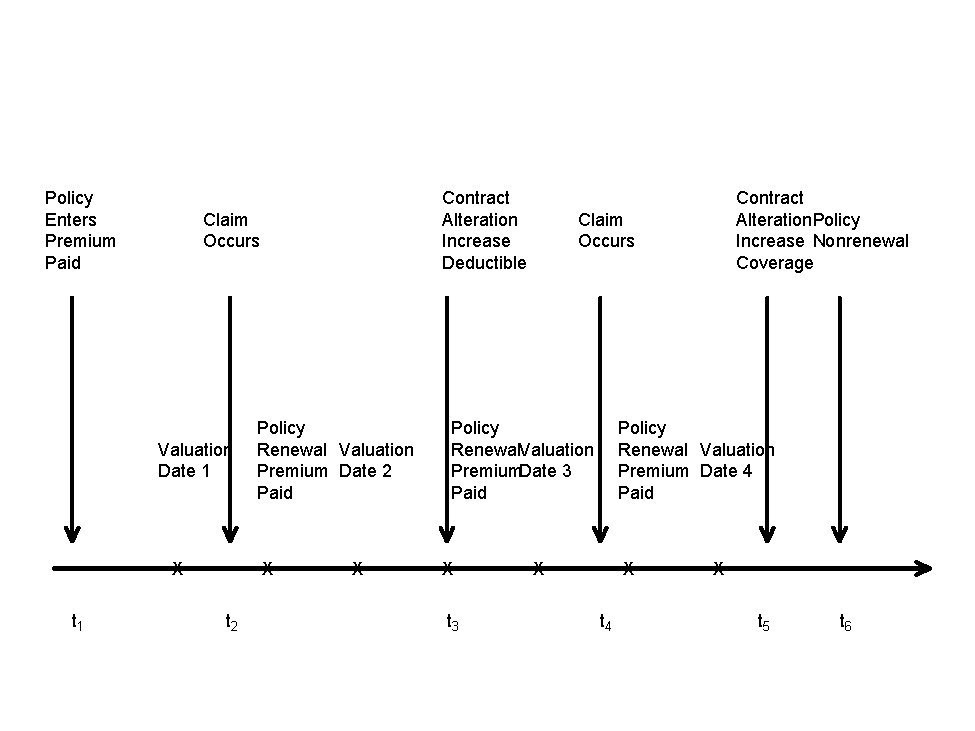
\includegraphics[width=1\linewidth]{LossDataAnalytics_files/figure-latex/StochOperations-1} 

}

\caption{\textbf{Timeline of a Typical Insurance Policy.} Arrows mark the occurrences of random events. Each x marks the time of scheduled events that are typically non-random.}\label{fig:StochOperations}
\end{figure}

\hypertarget{S:PredModApps}{%
\section{Insurance Company Operations}\label{S:PredModApps}}

\begin{center}\rule{0.5\linewidth}{0.5pt}\end{center}

In this section, you learn how to:

\begin{itemize}
\tightlist
\item
  Describe five major operational areas of insurance companies.
\item
  Identify the role of data and analytics opportunities within each operational area.
\end{itemize}

\begin{center}\rule{0.5\linewidth}{0.5pt}\end{center}

Armed with insurance data, the end goal is to use data to make decisions. We will learn more about methods of analyzing and extrapolating data in future chapters. To begin, let us think about why we want to do the analysis.
We take the insurance company's viewpoint (not the insured person) and introduce ways of bringing money in, paying it out, managing costs, and making sure that we have enough money to meet obligations. The emphasis is on insurance-specific operations rather than on general business activities such as advertising, marketing, and human resources management.

Specifically, in many insurance companies, it is customary to aggregate
detailed insurance processes into larger operational units; many
companies use these functional areas to segregate employee activities
and areas of responsibilities. Actuaries, other financial analysts, and insurance regulators work within these units and use data for the following activities:

\begin{enumerate}
\def\labelenumi{\arabic{enumi}.}
\tightlist
\item
  \textbf{Initiating Insurance}. At this stage, the company makes a
  decision as to whether or not to take on a risk (the
  underwriting stage) and assign an appropriate
  premium (or rate). Insurance analytics has its actuarial roots in \emph{ratemaking}, where
  analysts seek to determine the right price for the right risk.
\item
  \textbf{Renewing Insurance}. Many contracts, particularly in general
  insurance, have relatively short durations such as 6 months or
  a year. Although there is an implicit expectation that such
  contracts will be renewed, the insurer has the opportunity to
  decline coverage and to adjust the premium. Analytics is also used
  at this policy renewal stage where the goal is to retain
  profitable customers.
\item
  \textbf{Claims Management}. Analytics has long been used in (1) detecting
  and preventing claims fraud, (2) managing claim costs, including
  identifying the appropriate support for claims handling expenses, as
  well as (3) understanding excess layers for reinsurance
  and retention.
\item
  \textbf{Loss Reserving}. Analytic tools are used to provide management
  with an appropriate estimate of future obligations and to quantify
  the uncertainty of those estimates.
\item
  \textbf{Solvency and Capital Allocation}. Deciding on the requisite
  amount of capital and on ways of allocating capital among alternative
  investments are also important
  analytics activities. Companies must understand how much capital is
  needed so that they have sufficient flow of cash available to
  meet their obligations at the times they are expected to materialize (solvency). This is an important question that concerns
  not only company managers but also customers, company shareholders,
  regulatory authorities, as well as the public at large. Related to
  issues of how much capital is the question of how to allocate
  capital to differing financial projects, typically to maximize an
  investor's return. Although this question can arise at several
  levels, insurance companies are typically concerned with how to
  allocate capital to different lines of business within a firm and to
  different subsidiaries of a parent firm.
\end{enumerate}

Although data represent a critical component of solvency and capital
allocation, other components including the local and global economic framework, the financial investments environment, and quite specific requirements according to the regulatory environment of the day, are also important. Because of the
background needed to address these components, we do not address
solvency, capital allocation, and regulation issues in this text.

Nonetheless, for all operating functions, we emphasize that analytics in
the insurance industry is not an exercise that a small group of analysts
can do by themselves. It requires an insurer to make significant
investments in their information technology, marketing, underwriting,
and actuarial functions. As these areas represent the primary end goals
of the analysis of data, additional background on each operational unit
is provided in the following subsections.

\hypertarget{initiating-insurance}{%
\subsection{Initiating Insurance}\label{initiating-insurance}}

Setting the price of an insurance product can be a perplexing problem. This is in contrast to other industries such as manufacturing where the cost of a product is (relatively) known and provides a benchmark for assessing a market demand price. Similarly, in other areas of financial services, market prices are available and provide the basis
for a market-consistent pricing structure of products. However, for many lines of insurance, the cost of a product is uncertain and market prices are unavailable. Expectations of the random cost is a reasonable
place to start for a price. (If you have studied finance, then you will recall that an expectation is the optimal price for a risk-neutral insurer.) It has been traditional in insurance pricing to begin with the expected cost. Insurers then add margins to this, to account for the product's riskiness,
expenses incurred in servicing the product, and an allowance for profit/surplus of the company.

Use of expected costs as a foundation for pricing is prevalent in some lines of the insurance business. These include automobile and homeowners insurance. For these lines, analytics has served to sharpen the market by making the
calculation of the product's expected cost more precise. The increasing availability of the internet to consumers has also promoted transparency in pricing; in today's marketplace, consumers have ready access to competing quotes from a host of insurers. Insurers seek to increase their market share by refining their risk classification systems, thus achieving a better approximation of the products' prices and enabling cream-skimming underwriting strategies (``cream-skimming'' is a phrase used when the insurer underwrites only the best risks). Surveys (e.g., \citet{survey2013}) indicate that pricing is the most common use of analytics among insurers.

\emph{Underwriting}, the process of classifying risks into homogeneous
categories and assigning policyholders to these categories, lies at the
core of ratemaking. Policyholders within a class (category) have similar risk
profiles and so are charged the same insurance price. This is the
concept of an actuarially fair premium; it is fair to charge
different rates to policyholders only if they can be separated by
identifiable risk factors. An early article, \emph{Two Studies in Automobile Insurance Ratemaking} \citep{bailey1960}, provided a catalyst to the acceptance of analytic methods in the insurance industry. This paper addresses the problem of classification ratemaking.
It describes an example of automobile insurance that has five use
classes cross-classified with four merit rating classes. At that time,
the contribution to premiums for use and merit rating classes were
determined independently of each other. Thinking about the interacting
effects of different classification variables is a more difficult
problem.

When the risk is initially obtained, the insurer's obligations can be managed by imposing contract parameters that modify contract payouts. Chapter \ref{ChapSeverity} describes common modifications including coinsurance, deductibles and policy upper limits.

\hypertarget{renewing-insurance}{%
\subsection{Renewing Insurance}\label{renewing-insurance}}

Insurance is a type of financial service and, like many service
contracts, insurance coverage is often agreed upon for a limited time
period at which time coverage commitments are
complete. Particularly for general insurance, the need for coverage continues and so efforts are made to issue a new contract providing similar coverage when the existing contract comes to the end of its term. This is called \emph{policy renewal}. Renewal issues can also arise in life insurance, e.g.,
term (temporary) life insurance. At the same time other contracts, such as life
annuities, terminate upon the insured's death and so issues of
renewability are irrelevant.

In the absence of legal restrictions, at renewal the insurer has the opportunity to:

\begin{itemize}
\tightlist
\item
  accept or decline to underwrite the risk; and
\item
  determine a new premium, possibly in conjunction with a new
  classification of the risk.
\end{itemize}

Risk classification and rating at renewal is based on two types of information. First, at the initial stage, the insurer has available many rating variables upon which decisions can be made. Many variables are not likely to change, e.g., sex, whereas others are likely to change, e.g., age, and still others may or may not change, e.g., credit score. Second, unlike the initial stage, at renewal the insurer has available a history of policyholder's loss experience, and this history can provide insights into the policyholder that are not available from rating variables. Modifying premiums with claims history is known as \emph{experience rating}, also sometimes referred to as \emph{merit rating}.

Experience rating methods are either applied retrospectively or prospectively. With retrospective methods, a refund of a portion of the
premium is provided to the policyholder in the event of favorable (to the insurer) experience. Retrospective premiums are common in life insurance arrangements (where policyholders earn dividends in the U.S., bonuses in the U.K., and profit sharing in Israeli term life coverage). In general insurance, prospective methods are more common, where favorable insured experience is rewarded through a lower renewal premium.

Claims history can provide information about a policyholder's risk appetite. For example, in personal lines it is common to use a variable to indicate whether or not a claim has occurred in the last three years. As another example, in a commercial line such as worker's compensation, one may look to a policyholder's average claim frequency or severity over the last three years. Claims history can reveal information that is otherwise hidden (to the insurer) about the policyholder.

\hypertarget{claims-and-product-management}{%
\subsection{Claims and Product Management}\label{claims-and-product-management}}

In some of types of insurance, the process of paying claims for insured events is relatively straightforward. For example, in life insurance, a simple death certificate is all that is needed to pay the benefit amount as provided in the contract. However, in non-life areas such as property and casualty insurance, the process can be much more complex. Think about a relatively simple insured event such as an automobile accident. Here, it is often required to determine which party is at fault and then one needs to assess damage to all of the vehicles and people involved in the incident, both insured and non-insured. Further, the expenses incurred in assessing the damages must be assessed, and so forth. The process of determining coverage, legal liability, and settling claims is known as claims adjustment.

Insurance managers sometimes use the phrase claims leakage to mean dollars lost through claims management inefficiencies. There are many
ways in which analytics can help manage the claims process, c.f., \citet{SASsurvey}. Historically, the most important has been fraud detection.
The claim adjusting process involves reducing information asymmetry (the claimant knows what happened; the company knows some of what happened). Mitigating fraud is an important part of the claims management process.

Fraud detection is only one aspect of managing claims. More broadly, one can think about claims management as consisting of the following components:

\begin{itemize}
\tightlist
\item
  \textbf{Claims triaging}. Just as in the medical world, early identification and appropriate handling of high cost claims (patients, in the medical world), can lead to dramatic savings. For example, in workers compensation, insurers look to achieve early identification of those claims that run the risk of high medical costs and a long payout period. Early intervention into these cases could give insurers more control over the handling of the claim, the medical treatment, and the overall costs with an earlier return-to-work.
\item
  \textbf{Claims processing}. The goal is to use analytics to identify routine situations that are anticipated to have small payouts. More complex situations may require more experienced adjusters and legal assistance to appropriately handle claims with high potential payouts.
\item
  \textbf{Adjustment decisions}. Once a complex claim has been identified and assigned to an adjuster, analytic driven routines can be established to aid subsequent decision-making processes. Such processes can also be helpful for adjusters in developing case reserves, an estimate of the insurer's future liability. This is an important input to the insurer's loss reserves, described in Section \ref{S:Reserving}.
\end{itemize}

In addition to the insured's reimbursement for losses, the insurer also needs to be concerned with another source of revenue outflow, expenses. Loss adjustment expenses are part of an insurer's cost of managing claims. Analytics can be used to reduce expenses directly related to claims handling (allocated) as well as general staff time for overseeing the claims processes (unallocated). The insurance industry has high operating costs relative to other portions of the financial services sectors.

In addition to claims payments, there are many other ways in which insurers use data to manage their products. We have already discussed
the need for analytics in underwriting, that is, risk classification at the initial acquisition and renewal stages. Insurers are also interested in which policyholders elect to renew their contracts and, as with other products, monitor customer loyalty.

Analytics can also be used to manage the portfolio, or collection, of risks that an insurer has acquired. As described in Chapter \ref{ChapPortMgt}, after the contract has been agreed upon with an insured, the insurer may still modify its net obligation by entering into a reinsurance agreement. This type of agreement is with a reinsurer, an insurer of an insurer. It is common for insurance companies to purchase insurance on its portfolio of risks to gain protection from unusual events, just as people and other companies do.

\hypertarget{S:Reserving}{%
\subsection{Loss Reserving}\label{S:Reserving}}

An important feature that distinguishes insurance from other sectors of the economy is the timing of the exchange of considerations. In manufacturing, payments for goods are typically made at the time of a transaction. In contrast, for insurance, money received from a customer occurs in advance of benefits or services; these are rendered at a later date if the insured event occurs. This leads to the need to hold a reservoir of wealth to meet future obligations in respect to obligations made, and to gain the trust of the insureds that the company will be able to fulfill its commitments. The size of this reservoir of wealth, and the importance of ensuring its adequacy, is a major concern for the insurance industry.

Setting aside money for unpaid claims is known as loss reserving; in some jurisdictions, reserves are also known as \emph{technical provisions}. We saw in Figure \ref{fig:StochOperations} several times at which a company summarizes its financial position; these times are known as valuation dates. Claims that arise prior to valuation dates have either been paid, are in the process of being paid, or are about to be paid; claims in the future of these valuation dates are unknown. A company must estimate these outstanding liabilities when determining its financial strength. Accurately determining loss reserves is important to insurers for many reasons.

\begin{enumerate}
\def\labelenumi{\arabic{enumi}.}
\tightlist
\item
  Loss reserves represent an anticipated claim that the insurer owes its customers. Under-reserving may result in a failure to meet claim liabilities. Conversely, an insurer with excessive reserves may present a conservative estimate of surplus and thus portray a weaker financial position than it truly has.
\item
  Reserves provide an estimate for the unpaid cost of insurance that can be used for pricing contracts.
\item
  Loss reserving is required by laws and regulations. The public has a strong interest in the financial strength and solvency of insurers.
\item
  In addition to regulators, other stakeholders such as insurance company management, investors, and customers make decisions that depend on company loss reserves. Whereas regulators and customers appreciate conservative estimates of unpaid claims, managers and investors seek more unbiased estimates to represent the true financial health of the company.
\end{enumerate}

Loss reserving is a topic where there are substantive differences between life and general (also known as property and casualty, or non-life) insurance. In life insurance, the severity (amount of loss) is often not a source of uncertainty as payouts are specified in the contract. The frequency, driven by mortality of the insured, is a concern. However, because of the lengthy time for settlement of life insurance contracts, the time value of money uncertainty as measured
from issue to date of payment can dominate frequency concerns. For example, for an insured who purchases a life contract at age 20, it would not be unusual for the contract to still be open in 60 years time, when the insured celebrates his or her 80th birthday. See, for example, \citet{bowers1986actuarial} or \citet{dickson2013actuarial} for introductions to reserving for life insurance. In contrast, for most lines of non-life business, severity is a major source of uncertainty and contract durations tend to be shorter.

\hypertarget{S:LGPIF}{%
\section{Case Study: Wisconsin Property Fund}\label{S:LGPIF}}

\begin{center}\rule{0.5\linewidth}{0.5pt}\end{center}

In this section, we use the Wisconsin Property Fund as a case study. You learn how to:

\begin{itemize}
\tightlist
\item
  Describe how data generating events can produce data of interest to insurance analysts.
\item
  Produce relevant summary statistics for each variable.
\item
  Describe how these summary statistics can be used in each of the major operational areas of an insurance company.
\end{itemize}

\begin{center}\rule{0.5\linewidth}{0.5pt}\end{center}

Let us illustrate the kind of data under consideration and the goals that we wish to achieve by examining the Local Government Property Insurance Fund (LGPIF), an insurance pool administered by the Wisconsin Office of the Insurance Commissioner. The LGPIF was established to provide property insurance for local government entities that include counties, cities, towns, villages, school districts, and library boards. The fund insures local government property such as government buildings, schools, libraries, and motor vehicles. It covers all property losses except those resulting from flood, earthquake, wear and tear, extremes in temperature, mold, war, nuclear reactions, and embezzlement or theft by an employee.

The fund covers over a thousand local government entities who pay approximately 25 million dollars in premiums each year and receive insurance coverage of about 75 billion. State government buildings are not covered; the LGPIF is for local government entities that have separate budgetary responsibilities and who need insurance to moderate the budget effects of uncertain insurable events. Coverage for local government property has been made available by the State of Wisconsin since 1911, thus providing a wealth of historical data.

In this illustration, we restrict consideration to claims from coverage of building and contents; we do not consider claims from motor vehicles and specialized equipment owned by local entities (such as snow plowing machines). We also consider only claims that are closed, with obligations fully met.

\hypertarget{S:OutComes}{%
\subsection{Fund Claims Variables: Frequency and Severity}\label{S:OutComes}}

At a fundamental level, insurance companies accept premiums in exchange for promises to compensate a policyholder upon the occurrence
of an insured event. Indemnification is the compensation provided by the insurer for incurred hurt, loss, or damage that is covered by the policy. This compensation is also known as a \emph{claim}. The extent of the payout, known as the \emph{severity}, is a key financial expenditure for an insurer.

In terms of money outgo, an insurer is indifferent to having ten claims of 100 when compared to one claim of 1,000. Nonetheless, it is common for
insurers to study how often claims arise, known as the \emph{frequency} of
claims. The frequency is important for expenses, but it also influences
contractual parameters (such as deductibles and policy limits that are described later) that are
written on a per occurrence basis. Frequency is routinely monitored by insurance
regulators and can be a key driver in the overall indemnification
obligation of the insurer. We shall consider the frequency and severity as the two main claim variables that we wish to understand, model, and manage.

To illustrate, in 2010 there were 1,110 policyholders in the property fund who experienced a total of 1,377 claims. \protect\hyperlink{tab:1.1}{Table 1.1} shows the distribution. Almost two-thirds (0.637) of the policyholders did not have any claims and an additional 18.8\% had only one claim. The remaining 17.5\%
(=1 - 0.637 - 0.188) had more than one claim; the policyholder with the highest number recorded 239 claims. The average number of claims for
this sample was 1.24 (=1377/1110).

Table 1.1. \textbf{2010 Claims Frequency Distribution}

\begin{longtable}[]{@{}llllllllllll@{}}
\toprule
Type & & & & & & & & & & & \\
\midrule
\endhead
Number & 0 & 1 & 2 & 3 & 4 & 5 & 6 & 7 & 8 & 9 or more & Sum \\
Policies & 707 & 209 & 86 & 40 & 18 & 12 & 9 & 4 & 6 & 19 & 1,110 \\
Claims & 0 & 209 & 172 & 120 & 72 & 60 & 54 & 28 & 48 & 617 & 1,377 \\
Proportion & 0.637 & 0.188 & 0.077 & 0.036 & 0.016 & 0.011 & 0.008 & 0.004 & 0.005 & 0.017 & 1.000 \\
\bottomrule
\end{longtable}

For the severity distribution, a common approach is to examine the distribution of the sample of 1,377 claims. However, another common
approach is to examine the distribution of the average claims of those policyholders with claims. In our 2010 sample, there were 403
(=1110-707) such policyholders. For 209 of these policyholders with one claim, the average claim equals the only claim they experienced. For the
policyholder with highest frequency, the average claim is an average over 239 separately reported claim events. This average is also known as the
pure premium or \emph{loss cost}.

\protect\hyperlink{tab:1.2}{Table 1.2} summarizes the sample distribution of average severities from the 403 policyholders who made a claim; it shows that the average claim amount was 56,330 (all amounts are in U.S. Dollars). However, the average gives only a limited look at the distribution. More information can be
gleaned from the summary statistics which show a very large claim in the amount of 12,920,000. Figure \ref{fig:SeverityFig} provides further
information about the distribution of sample claims, showing a distribution that is dominated by this single large claim so that the
histogram is not very helpful. Even when removing the large claim, you will find a distribution that is skewed to the right. A generally
accepted technique is to work with claims in logarithmic units especially for graphical purposes; the corresponding figure in the
right-hand panel is much easier to interpret.

Table 1.2. \textbf{2010 Average Severity Distribution}

\begin{longtable}[]{@{}
  >{\raggedleft\arraybackslash}p{(\columnwidth - 10\tabcolsep) * \real{0.14}}
  >{\raggedleft\arraybackslash}p{(\columnwidth - 10\tabcolsep) * \real{0.15}}
  >{\raggedleft\arraybackslash}p{(\columnwidth - 10\tabcolsep) * \real{0.12}}
  >{\raggedleft\arraybackslash}p{(\columnwidth - 10\tabcolsep) * \real{0.12}}
  >{\raggedleft\arraybackslash}p{(\columnwidth - 10\tabcolsep) * \real{0.15}}
  >{\raggedleft\arraybackslash}p{(\columnwidth - 10\tabcolsep) * \real{0.18}}@{}}
\toprule
Minimum & First
Quartile & Median & Mean & Third
Quartile & Maximum \\
\midrule
\endhead
167 & 2,226 & 4,951 & 56,330 & 11,900 & 12,920,000 \\
\bottomrule
\end{longtable}



\begin{figure}

{\centering 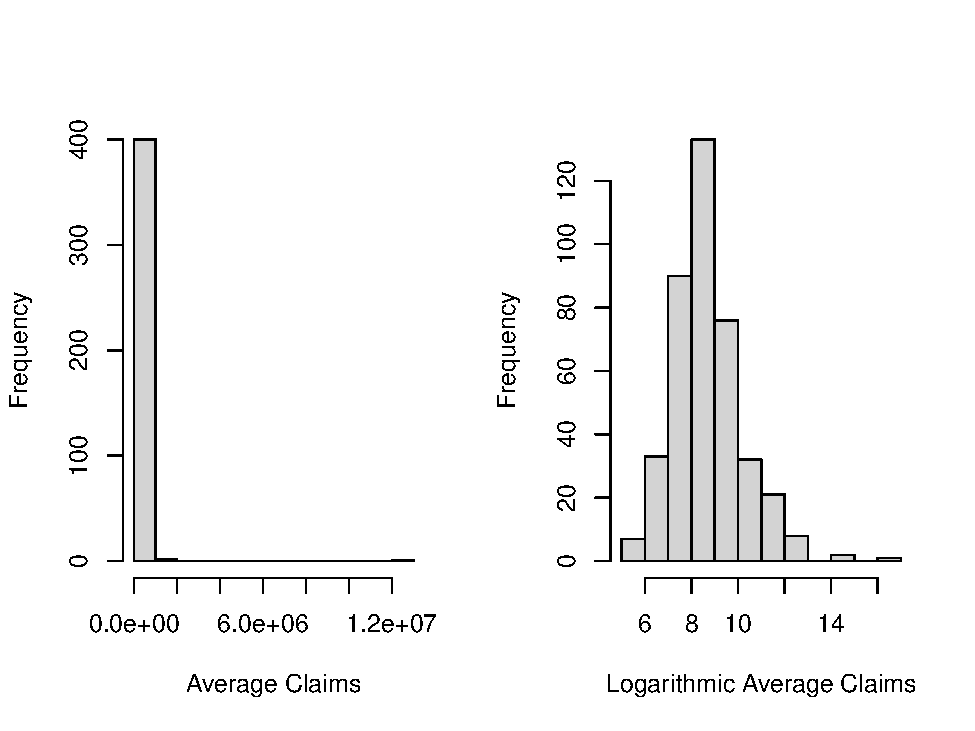
\includegraphics[width=0.8\linewidth]{LossDataAnalytics_files/figure-latex/SeverityFig-1} 

}

\caption{\textbf{Distribution of Positive Average Severities}}\label{fig:SeverityFig}
\end{figure}

\hypertarget{S:FundVariables}{%
\subsection{Fund Rating Variables}\label{S:FundVariables}}

Developing models to represent and manage the two outcome variables,
frequency and severity, is the focus of the early chapters of this text.
However, when actuaries and other financial analysts use those models,
they do so in the context of external variables. In general
statistical terminology, one might call these explanatory or predictor
variables; there are many other names in statistics, economics,
psychology, and other disciplines. Because of our insurance focus, we
call them rating variables as they are useful in setting insurance rates and premiums.

We earlier considered observations from a sample of 1,110 policyholders which may seem like
a lot. However, as we will see in our forthcoming applications, because
of the preponderance of zeros and the skewed nature of claims, actuaries
typically yearn for more data. One common approach that we adopt here is
to examine outcomes from multiple years, thus increasing the sample
size. We will discuss the strengths and limitations of this strategy
later but, at this juncture, we just wish to show the reader how it works.

Specifically, \protect\hyperlink{tab:1.3}{Table 1.3} shows that we now consider
policies over five years of data, 2006, \ldots, 2010, inclusive. The
data begins in 2006 because there was a shift in claim coding in 2005 so
that comparisons with earlier years are not helpful. To mitigate the
effect of open claims, we consider policy years prior to 2011. An open
claim means that not all of the obligations for the claim are known at the time of the analysis; for some claims, such an injury to a person in an auto
accident or in the workplace, it can take years before costs are fully
known.

Table 1.3. \textbf{Claims Summary by Policyholder}

\begin{longtable}[]{@{}
  >{\raggedright\arraybackslash}p{(\columnwidth - 8\tabcolsep) * \real{0.19}}
  >{\raggedleft\arraybackslash}p{(\columnwidth - 8\tabcolsep) * \real{0.17}}
  >{\raggedleft\arraybackslash}p{(\columnwidth - 8\tabcolsep) * \real{0.19}}
  >{\raggedleft\arraybackslash}p{(\columnwidth - 8\tabcolsep) * \real{0.18}}
  >{\raggedleft\arraybackslash}p{(\columnwidth - 8\tabcolsep) * \real{0.19}}@{}}
\toprule
Year & Average
Frequency & Average
Severity & Average
Coverage & Number of
Policyholders \\
\midrule
\endhead
2006 & 0.951 & 9,695 & 32,498,186 & 1,154 \\
2007 & 1.167 & 6,544 & 35,275,949 & 1,138 \\
2008 & 0.974 & 5,311 & 37,267,485 & 1,125 \\
2009 & 1.219 & 4,572 & 40,355,382 & 1,112 \\
2010 & 1.241 & 20,452 & 41,242,070 & 1,110 \\
\bottomrule
\end{longtable}

\protect\hyperlink{tab:1.3}{Table 1.3} shows that the average claim varies over time,
especially with the high 2010 value (that we saw was due to a single large claim)\footnote{Note that the average severity in \protect\hyperlink{tab:1.3}{Table 1.3} differs from that reported in \protect\hyperlink{tab:1.2}{Table 1.2}. This is because the former includes policyholders with zero claims where as the latter does not. This is an important distinction that we will address in later portions of the text.}. The
total number of policyholders is steadily declining and, conversely, the
coverage is steadily increasing. The coverage variable is the amount of
coverage of the property and contents. Roughly, you can think of it as
the maximum possible payout of the insurer. For our immediate purposes,
the coverage is our first rating variable. Other things being equal, we would
expect that policyholders with larger coverage have larger claims.
We will make this vague idea much more precise as we proceed, and also justify this expectation with data.

For a different look at the 2006-2010 data, \protect\hyperlink{tab:1.4}{Table 1.4}
summarizes the distribution of our two outcomes, frequency and claims
amount. In each case, the average exceeds the median, suggesting that
the two distributions are right-skewed. In addition, the table
summarizes our continuous rating variables, coverage and deductible
amount. The table also suggests that these variables also have
right-skewed distributions.

Table 1.4. \textbf{Summary of Claim Frequency and Severity, Deductibles, and Coverages}

\begin{longtable}[]{@{}
  >{\raggedright\arraybackslash}p{(\columnwidth - 8\tabcolsep) * \real{0.26}}
  >{\raggedleft\arraybackslash}p{(\columnwidth - 8\tabcolsep) * \real{0.14}}
  >{\raggedleft\arraybackslash}p{(\columnwidth - 8\tabcolsep) * \real{0.12}}
  >{\raggedleft\arraybackslash}p{(\columnwidth - 8\tabcolsep) * \real{0.14}}
  >{\raggedleft\arraybackslash}p{(\columnwidth - 8\tabcolsep) * \real{0.18}}@{}}
\toprule
& Minimum & Median & Average & Maximum \\
\midrule
\endhead
Claim Frequency & 0 & 0 & 1.109 & 263 \\
Claim Severity & 0 & 0 & 9,292 & 12,922,218 \\
Deductible & 500 & 1,000 & 3,365 & 100,000 \\
Coverage (000's) & 8.937 & 11,354 & 37,281 & 2,444,797 \\
\bottomrule
\end{longtable}

\protect\hyperlink{tab:1.5}{Table 1.5} describes the rating variables considered in this chapter. Hopefully, these are variables that you think might naturally be related to claims outcomes. You can learn more about them in \citet{frees2016multivariate}. To handle the skewness, we henceforth focus on logarithmic transformations of coverage and deductibles.

Table 1.5. \textbf{Description of Rating Variables}

\[{\small \begin{matrix}
\begin{array}{ l | l}
\hline
Variable    & Description \\
\hline
\text{EntityType}   & \text{Categorical variable that is one of six types:  (Village, City,} \\
& ~~~~ \text{County, Misc, School, or Town)} \\
\text{LnCoverage}   & \text{Total building and content coverage, in logarithmic millions of dollars}\\
\text{LnDeduct}     & \text{Deductible, in logarithmic dollars} \\
\text{AlarmCredit}  & \text{Categorical variable that is one of four types:  (0, 5, 10, or 15)} \\
 &  ~~~~   \text{for automatic smoke alarms in main rooms} \\
\text{NoClaimCredit}    & \text{Binary variable to indicate no claims in the past two years} \\
\text{Fire5 }           & \text{Binary variable to indicate the fire class is below 5} \\
& ~~~~ \text{(The range of fire class is 0 to 10)} \\
\hline
\end{array}
\end{matrix}}\]

To get a sense of the relationship between the non-continuous rating variables and claims, \href{../docs/ChapIntro.html\#tab:1.6}{Table 1.6} relates the claims outcomes to these
categorical variables. \href{../docs/ChapIntro.html\#tab:1.6}{Table 1.6} suggests substantial variation in the claim frequency and average severity of the claims by
entity type. It also demonstrates higher frequency and severity for the
\({\tt Fire5}\) variable and the reverse for the \({\tt NoClaimCredit}\) variable.
The relationship for the \({\tt Fire5}\) variable is counter-intuitive in that
one would expect lower claim amounts for those policyholders in areas
with better public protection (when the protection code is five or
less). Naturally, there are other variables that influence this
relationship. We will see that these background variables are accounted
for in the subsequent multivariate regression analysis, which yields an
intuitive, appealing (negative) sign for the \({\tt Fire5}\) variable.

Table 1.6. \textbf{Claims Summary by Entity Type, Fire Class, and No Claim Credit}

\begin{longtable}[]{@{}
  >{\raggedright\arraybackslash}p{(\columnwidth - 6\tabcolsep) * \real{0.31}}
  >{\raggedleft\arraybackslash}p{(\columnwidth - 6\tabcolsep) * \real{0.17}}
  >{\raggedleft\arraybackslash}p{(\columnwidth - 6\tabcolsep) * \real{0.17}}
  >{\raggedleft\arraybackslash}p{(\columnwidth - 6\tabcolsep) * \real{0.17}}@{}}
\toprule
Variable & Number of
Policies & Claim
Frequency & Average
Severity \\
\midrule
\endhead
\emph{EntityType} & & & \\
Village & 1,341 & 0.452 & 10,645 \\
City & 793 & 1.941 & 16,924 \\
County & 328 & 4.899 & 15,453 \\
Misc & 609 & 0.186 & 43,036 \\
School & 1,597 & 1.434 & 64,346 \\
Town & 971 & 0.103 & 19,831 \\
\emph{Fire} & & & \\
Fire5=0 & 2,508 & 0.502 & 13,935 \\
Fire5=1 & 3,131 & 1.596 & 41,421 \\
\emph{No Claims Credit} & & & \\
NoClaimCredit=0 & 3,786 & 1.501 & 31,365 \\
NoClaimCredit=1 & 1,853 & 0.310 & 30,499 \\
\textbf{Total} & 5,639 & 1.109 & 31,206 \\
\bottomrule
\end{longtable}

\protect\hyperlink{tab:1.7}{Table 1.7} shows the claims experience by alarm credit.
It underscores the difficulty of examining variables individually. For
example, when looking at the experience for all entities, we see that
policyholders with no alarm credit have on average lower frequency and
severity than policyholders with the highest (15\%, with 24/7 monitoring
by a fire station or security company) alarm credit. In particular, when
we look at the entity type School, the frequency is 0.422 and the
severity 25,523 for no alarm credit, whereas for the highest alarm level
it is 2.008 and 85,140, respectively. This may simply imply that entities with more claims are the ones that are likely to have an alarm system. Summary
tables do not examine multivariate effects; for example, \href{../docs/ChapIntro.html\#tab:1.6}{Table 1.6} ignores the effect of size (as we measure through
coverage amounts) that affect claims.

Table 1.7. \textbf{Claims Summary by Entity Type and Alarm Credit (AC) Category}

\begin{longtable}[]{@{}
  >{\raggedright\arraybackslash}p{(\columnwidth - 12\tabcolsep) * \real{0.12}}
  >{\raggedleft\arraybackslash}p{(\columnwidth - 12\tabcolsep) * \real{0.15}}
  >{\raggedleft\arraybackslash}p{(\columnwidth - 12\tabcolsep) * \real{0.14}}
  >{\raggedleft\arraybackslash}p{(\columnwidth - 12\tabcolsep) * \real{0.14}}
  >{\raggedleft\arraybackslash}p{(\columnwidth - 12\tabcolsep) * \real{0.15}}
  >{\raggedleft\arraybackslash}p{(\columnwidth - 12\tabcolsep) * \real{0.14}}
  >{\raggedleft\arraybackslash}p{(\columnwidth - 12\tabcolsep) * \real{0.14}}@{}}
\toprule
Entity
Type & AC0
Claim
Frequency & AC0
Avg.
Severity & AC0
Num.
Policies & AC5
Claim
Frequency & AC5
Avg.
Severity & AC5
Num.
Policies \\
\midrule
\endhead
Village & 0.326 & 11,078 & 829 & 0.278 & 8,086 & 54 \\
City & 0.893 & 7,576 & 244 & 2.077 & 4,150 & 13 \\
County & 2.140 & 16,013 & 50 & - & - & 1 \\
Misc & 0.117 & 15,122 & 386 & 0.278 & 13,064 & 18 \\
School & 0.422 & 25,523 & 294 & 0.410 & 14,575 & 122 \\
Town & 0.083 & 25,257 & 808 & 0.194 & 3,937 & 31 \\
Total & 0.318 & 15,118 & 2,611 & 0.431 & 10,762 & 239 \\
\bottomrule
\end{longtable}

\begin{longtable}[]{@{}
  >{\raggedright\arraybackslash}p{(\columnwidth - 12\tabcolsep) * \real{0.12}}
  >{\raggedleft\arraybackslash}p{(\columnwidth - 12\tabcolsep) * \real{0.15}}
  >{\centering\arraybackslash}p{(\columnwidth - 12\tabcolsep) * \real{0.14}}
  >{\raggedleft\arraybackslash}p{(\columnwidth - 12\tabcolsep) * \real{0.14}}
  >{\raggedleft\arraybackslash}p{(\columnwidth - 12\tabcolsep) * \real{0.15}}
  >{\raggedleft\arraybackslash}p{(\columnwidth - 12\tabcolsep) * \real{0.14}}
  >{\raggedleft\arraybackslash}p{(\columnwidth - 12\tabcolsep) * \real{0.14}}@{}}
\toprule
Entity
Type & AC10
Claim
Frequency & AC10
Avg.
Severity & AC10
Num.
Policies & AC15
Claim
Frequency & AC15
Avg.
Severity & AC15
Num.
Policies \\
\midrule
\endhead
Village & 0.500 & 8,792 & 50 & 0.725 & 10,544 & 408 \\
City & 1.258 & 8,625 & 31 & 2.485 & 20,470 & 505 \\
County & 2.125 & 11,688 & 8 & 5.513 & 15,476 & 269 \\
Misc & 0.077 & 3,923 & 26 & 0.341 & 87,021 & 179 \\
School & 0.488 & 11,597 & 168 & 2.008 & 85,140 & 1,013 \\
Town & 0.091 & 2,338 & 44 & 0.261 & 9,490 & 88 \\
Total & 0.517 & 10,194 & 327 & 2.093 & 41,458 & 2,462 \\
\bottomrule
\end{longtable}

We will learn more about modeling count data in the Chapter \ref{ChapFrequency-Modeling} and about severity data in Chapters \ref{ChapSeverity} and \ref{ChapAggLossModels}.

\hypertarget{fund-operations}{%
\subsection{Fund Operations}\label{fund-operations}}

We have now seen distributions of the Fund's two outcome variables: a count variable for the number of claims, and a continuous variable for the claims amount. We have also introduced a continuous rating variable (coverage); a discrete quantitative variable (logarithmic deductibles); two binary rating variables (no claims credit and fire class); and two categorical rating variables (entity type and alarm credit). Subsequent chapters will
explain how to analyze and model the distribution of these variables and their relationships. Before getting into these technical details, let us
first think about where we want to go. General insurance company functional areas are described in Section \ref{S:PredModApps}; we now consider how these areas might apply in the context of the property fund.

\hypertarget{initiating-insurance-1}{%
\subsubsection*{Initiating Insurance}\label{initiating-insurance-1}}
\addcontentsline{toc}{subsubsection}{Initiating Insurance}

Because this is a government sponsored fund, we do not have to worry
about selecting good or avoiding poor risks; the fund is not allowed to
deny a coverage application from a qualified local government entity. If
we do not have to underwrite, what about how much to charge?

We might look at the most recent experience in 2010, where the total
fund claims were approximately 28.16 million USD
(\(=1377 \text{ claims} \times 20452 \text{ average severity}\)). Dividing
that among 1,110 policyholders, that suggests a rate of 24,370 (
\(\approx\) 28,160,000/1110). However, 2010 was a bad year; using the same
method, our premium would be much lower based on 2009 data. This swing
in premiums would defeat the primary purpose of the fund, to allow for a
steady charge that local property managers could utilize in their
budgets.

Having a single price for all policyholders is nice but hardly seems
fair. For example, \href{../docs/ChapIntro.html\#tab:1.6}{Table 1.6} suggests that schools have
higher aggregate claims than other entities and so should pay more. However,
simply doing the calculation on an entity by entity basis is not right
either. For example, we saw in \protect\hyperlink{tab:1.7}{Table 1.7} that had we
used this strategy, entities with a 15\% alarm credit (for good behavior,
having top alarm systems) would actually wind up paying more.

So, we have the data for thinking about the appropriate rates to charge
but need to dig deeper into the analysis. We will explore this
topic further in Chapter \ref{ChapPremiumFoundations} on \emph{premium calculation fundamentals}.
Selecting appropriate risks is introduced in Chapter \ref{ChapRiskClass} on \emph{risk
classification}.

\hypertarget{renewing-insurance-1}{%
\subsubsection*{Renewing Insurance}\label{renewing-insurance-1}}
\addcontentsline{toc}{subsubsection}{Renewing Insurance}

Although property insurance is typically a one-year contract, \protect\hyperlink{tab:1.3}{Table 1.3} suggests that policyholders tend to renew; this is
typical of general insurance. For renewing policyholders, in addition to
their rating variables we have their claims history and this claims
history can be a good predictor of future claims. For example,
\href{../docs/ChapIntro.html\#tab:1.6}{Table 1.6} shows that policyholders without a claim in the last
two years had much lower claim frequencies than those with at least one
accident (0.310 compared to 1.501); a lower predicted frequency
typically results in a lower premium. This is why it is common for
insurers to use variables such as \({\tt NoClaimCredit}\) in their rating. We
will explore this topic further in Chapters \ref{ChapCredibility} and \ref{ChapBonusMalus} on \emph{experience rating}.

\hypertarget{claims-management}{%
\subsubsection*{Claims Management}\label{claims-management}}
\addcontentsline{toc}{subsubsection}{Claims Management}

Of course, the main story line of the 2010 experience was the large claim of
over 12 million USD, nearly half the amount of claims for that year. Are there
ways that this could have been prevented or mitigated? Are their ways
for the fund to purchase protection against such large unusual events?
Another unusual feature of the 2010 experience noted earlier was the
very large frequency of claims (239) for one policyholder. Given that
there were only 1,377 claims that year, this means that a single
policyholder had 17.4 \% of the claims. These extreme features of the data suggests
opportunities for managing claims, the subject of Chapter \ref{ChapPortMgt}.

\hypertarget{loss-reserving}{%
\subsubsection*{Loss Reserving}\label{loss-reserving}}
\addcontentsline{toc}{subsubsection}{Loss Reserving}

In our case study, we look only at the one year outcomes of closed
claims (the opposite of open). However, like many lines of insurance,
obligations from insured events to buildings such as fire, hail, and the
like, are not known immediately and may develop over time. Other lines
of business, including those where there are injuries to people, take
much longer to develop. Chapter \ref{ChapLossReserves} introduces this concern and \emph{loss reserving}, the discipline of determining how much the insurance company should retain to meet its obligations.

\hypertarget{exercises}{%
\section{Exercises}\label{exercises}}

These exercises ask you to work with data using statistical software, such as \texttt{R} code. If you would like some practice with \texttt{R} code, please visit the \href{https://openacttexts.github.io/LDACourse1/introduction-to-loss-data-analytics.html}{first chapter of a \emph{Short Course on Loss Data Analytics}}. As another method of learning, you can also get practice executing `R' code at our \href{https://openacttexts.github.io/LDARcode/}{Online Version R Code Site}.

\textbf{Exercise 1.1. Corporate Travel.} Universities purchase corporate travel policies to cover employees and students traveling on official university business for a wide variety of accidents and incidents while away from the campus or primary workplace. This broad coverage includes medical care and evacuation, loss of personal property, extraction for political and weather related reasons, and more. These data represent experience from the Australian National University (ANU) and additional details can be found in \href{https://services.anu.edu.au/files/document-collection/TRAVEL\%20INFORMATION\%20-\%20Travel\%20Information\%20Kit_July\%202018.pdf}{ANU's corporate travel policy}. You can also learn more about this line of business from ANU's insurer, \href{https://www.chubb.com/au-en/business/business-travel-group-travel-insurance.html}{Chubb Travel}. The data provided are maintained by the insurer, Chubb, and were accessed on 29 July 2022. You can retrieve the data by going to Appendix Section \ref{Sec:DataTravel}.

\emph{a. Claim Frequency.} The travel data history is long and stable. This coverage began on 1 November 2006. Table \ref{tab:TravelClaims1} shows the count of claims for years 2015-2019, inclusive. Produce a comparable table of claims frequency for the entire period. Comment on the unusual frequency surrounding the COVID pandemic.

\begin{table}

\caption{\label{tab:TravelClaims1}**2015-2019 Travel Claims Frequency**}
\centering
\begin{tabular}[t]{c|c|c|c|c}
\hline
2015 & 2016 & 2017 & 2018 & 2019\\
\hline
158 & 154 & 139 & 205 & 274\\
\hline
\end{tabular}
\end{table}

\begin{table}

\caption{\label{tab:TravelClaims1}\textbf{2015-2019 Travel Claims Frequency}}
\centering
\fontsize{10}{12}\selectfont
\begin{tabular}[t]{c>{\centering\arraybackslash}p{1.6cm}>{\centering\arraybackslash}p{1.6cm}>{\centering\arraybackslash}p{1.6cm}>{\centering\arraybackslash}p{1.6cm}>{}p{1.6cm}}
\toprule
2015 & 2016 & 2017 & 2018 & 2019\\
\midrule
\cellcolor{gray!6}{158} & \cellcolor{gray!6}{154} & \cellcolor{gray!6}{139} & \cellcolor{gray!6}{205} & \cellcolor{gray!6}{274}\\
\bottomrule
\end{tabular}
\end{table}

\emph{b. Adjust for Zero Claims.} From this data set, there are 2107 incurred claims. Of these claims, there are 269 zeros and an additional 3 claims where the incurred claim is less than 10. We omit these claims in our analysis. Reproduce your part (a) analysis by omitting incurred claims less than 10.

\emph{c.~Loss Distributions over Time.} There are 1835 incurred losses in the dataset with all available years (yet omitting claims less than 10). Figure \ref{fig:TravelClaims2} shows that the distribution of incurred losses is stable over the period 2015-2019, inclusive. Produce a comparable figure for the entire period.

\begin{figure}

{\centering 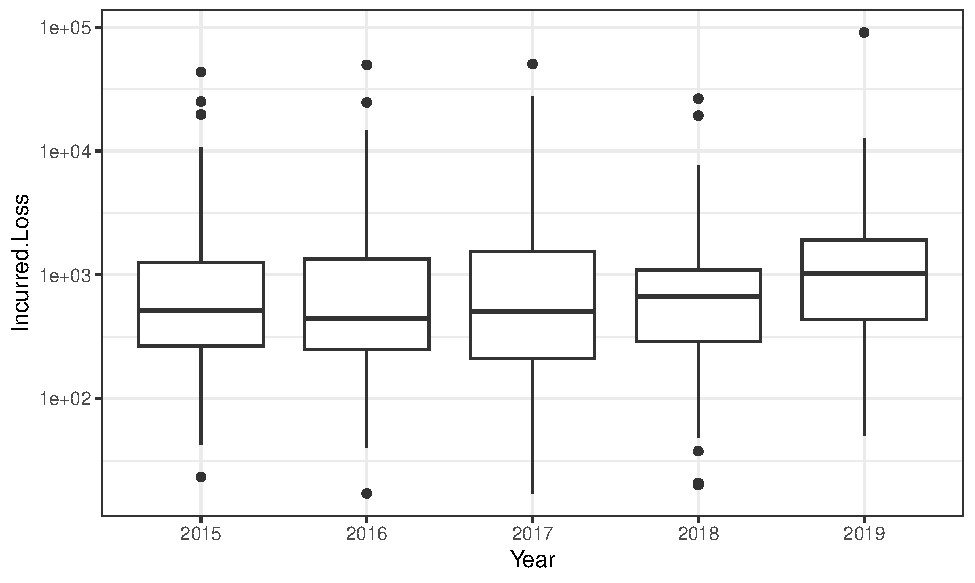
\includegraphics[width=0.6\linewidth]{LossDataAnalytics_files/figure-latex/TravelClaims2-1} 

}

\caption{**Distribution of Travel Losses by Year**}\label{fig:TravelClaims2}
\end{figure}

\emph{d.~Summary Statistics.} In addition to graphs, it can be helpful to display several summary statistics. For the five year period 2015-2019, produce a set of summary statistics.

\begin{Shaded}
\begin{Highlighting}[]
\CommentTok{\# a}
\NormalTok{TravelClaims }\OtherTok{\textless{}{-}} \FunctionTok{read.csv}\NormalTok{(}\StringTok{"Data/ANUTravelClaims2022.csv"}\NormalTok{, }\AttributeTok{header =}\NormalTok{ T)}
\NormalTok{tableTravel }\OtherTok{\textless{}{-}} \FunctionTok{t}\NormalTok{(}\FunctionTok{table}\NormalTok{(TravelClaims}\SpecialCharTok{$}\NormalTok{UW.Year))}
\NormalTok{knitr}\SpecialCharTok{::}\FunctionTok{kable}\NormalTok{(tableTravel, }\AttributeTok{align =} \StringTok{"cccccccc"}\NormalTok{, }\AttributeTok{caption =} \StringTok{"**Travel Claims Frequency**"}\NormalTok{)}
\end{Highlighting}
\end{Shaded}

\begin{table}

\caption{\label{tab:unnamed-chunk-18}**Travel Claims Frequency**}
\centering
\begin{tabular}[t]{c|c|c|c|c|c|c|c|c|c|c|c|c|c|c|c}
\hline
2006 & 2007 & 2008 & 2009 & 2010 & 2011 & 2012 & 2013 & 2014 & 2015 & 2016 & 2017 & 2018 & 2019 & 2020 & 2021\\
\hline
41 & 74 & 102 & 166 & 158 & 141 & 143 & 161 & 158 & 158 & 154 & 139 & 205 & 274 & 1 & 32\\
\hline
\end{tabular}
\end{table}

\begin{Shaded}
\begin{Highlighting}[]
\CommentTok{\# b}
\NormalTok{TravelClaimsGT10 }\OtherTok{\textless{}{-}} \FunctionTok{subset}\NormalTok{(TravelClaims, Incurred.Loss }\SpecialCharTok{\textgreater{}=} \DecValTok{10}\NormalTok{)}
\NormalTok{tableTravel1 }\OtherTok{\textless{}{-}} \FunctionTok{t}\NormalTok{(}\FunctionTok{table}\NormalTok{(TravelClaimsGT10}\SpecialCharTok{$}\NormalTok{UW.Year))}
\NormalTok{knitr}\SpecialCharTok{::}\FunctionTok{kable}\NormalTok{(tableTravel1, }\AttributeTok{align =} \StringTok{"cccccccc"}\NormalTok{, }\AttributeTok{caption =} \StringTok{"**Travel Claims Frequency**"}\NormalTok{)}
\end{Highlighting}
\end{Shaded}

\begin{table}

\caption{\label{tab:unnamed-chunk-18}**Travel Claims Frequency**}
\centering
\begin{tabular}[t]{c|c|c|c|c|c|c|c|c|c|c|c|c|c|c}
\hline
2006 & 2007 & 2008 & 2009 & 2010 & 2011 & 2012 & 2013 & 2014 & 2015 & 2016 & 2017 & 2018 & 2019 & 2021\\
\hline
31 & 58 & 86 & 154 & 153 & 136 & 135 & 140 & 132 & 142 & 132 & 129 & 170 & 207 & 30\\
\hline
\end{tabular}
\end{table}

\begin{Shaded}
\begin{Highlighting}[]
\CommentTok{\# c}

\FunctionTok{ggplot}\NormalTok{(}\AttributeTok{data =}\NormalTok{ TravelClaimsGT10, }\FunctionTok{aes}\NormalTok{(}\AttributeTok{x =} \FunctionTok{factor}\NormalTok{(UW.Year), }\AttributeTok{y =}\NormalTok{ Incurred.Loss)) }\SpecialCharTok{+} \FunctionTok{geom\_boxplot}\NormalTok{() }\SpecialCharTok{+}
    \FunctionTok{theme\_bw}\NormalTok{() }\SpecialCharTok{+} \FunctionTok{xlab}\NormalTok{(}\StringTok{"Year"}\NormalTok{) }\SpecialCharTok{+} \FunctionTok{scale\_y\_continuous}\NormalTok{(}\AttributeTok{trans =} \StringTok{"log10"}\NormalTok{)}
\end{Highlighting}
\end{Shaded}

\begin{center}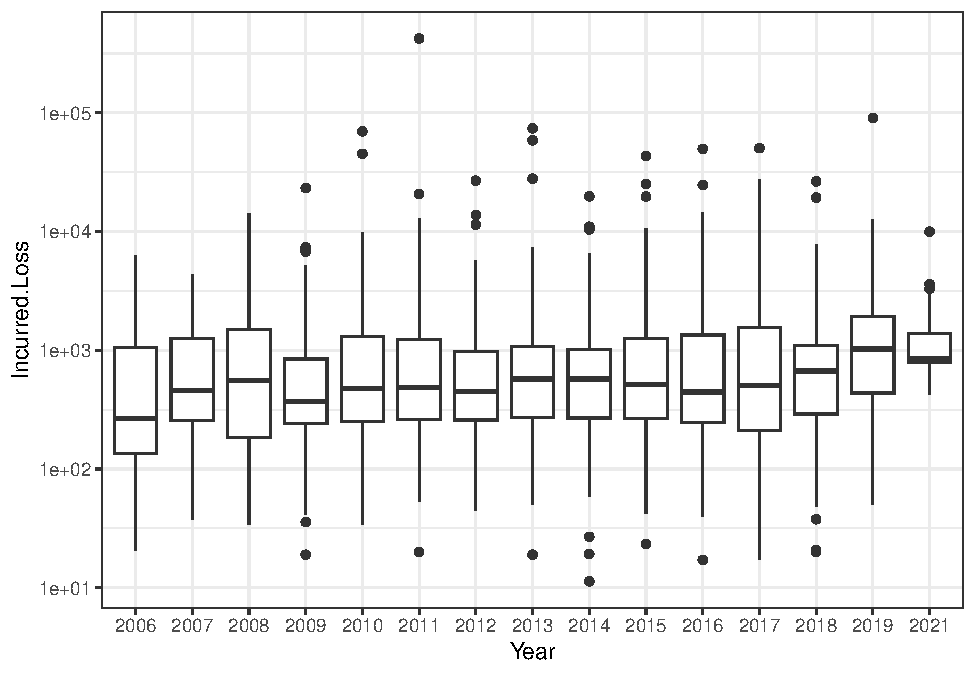
\includegraphics{LossDataAnalytics_files/figure-latex/unnamed-chunk-18-1} \end{center}

\begin{Shaded}
\begin{Highlighting}[]
\CommentTok{\# d}

\NormalTok{sumTravelClaims }\OtherTok{\textless{}{-}} \FunctionTok{t}\NormalTok{(}\FunctionTok{summary}\NormalTok{(TravelClaimsGT10Short}\SpecialCharTok{$}\NormalTok{Incurred.Loss))}
\NormalTok{knitr}\SpecialCharTok{::}\FunctionTok{kable}\NormalTok{(sumTravelClaims, }\AttributeTok{align =} \StringTok{"cccccccc"}\NormalTok{, }\AttributeTok{caption =} \StringTok{"**Travel Claims Summary Statistics**"}\NormalTok{)}
\end{Highlighting}
\end{Shaded}

\begin{table}

\caption{\label{tab:unnamed-chunk-18}**Travel Claims Summary Statistics**}
\centering
\begin{tabular}[t]{c|c|c|c|c|c}
\hline
Min. & 1st Qu. & Median & Mean & 3rd Qu. & Max.\\
\hline
17.16 & 290.215 & 631.49 & 1701.953 & 1528.44 & 90727.64\\
\hline
\end{tabular}
\end{table}

\begin{center}\rule{0.5\linewidth}{0.5pt}\end{center}

\textbf{Exercise 1.2. Group Personal Accident.} Group personal accident insurance offers financial protection in case of injury or death resulting from an incident that occurs on the job. Group personal accident offers insurance coverage and liability insurance protection against accidental death or injury. The insurance covers students and ANU's voluntary workers; ANU workers are covered through another system known as ``workers' compensation.''

Several limits apply including 1,000,000 for the period of insurance, 600,000 for non-scheduled flights, and others. These limits were not reached in the data we consider. For this coverage, there is a ``7 day excess'' for weekly benefits but none for general benefits. The database documentation provided to us, and the data we provide, do not indicate whether the excess has been triggered; we have only paid claims. Because of the relatively small size of this class of insurance, we ignore the effects of deductibles for this line.

The data provided to us are maintained by the insurer, Chubb. These data began in underwriting year 2007 and were accessed on 29 July 2022. You can retrieve the data by going to Appendix Section \ref{Sec:DataGPA}.

\emph{a. Claim Frequency.} From this data set, there are 148 incurred claims. Of these claims, there are 35 zeros and an additional 0 claims where the incurred claim is less than 10. We omit these claims in our analysis. Table \ref{tab:GPAFreq1} shows the count of claims for years 2015-2019, inclusive. Produce a comparable table of claims frequency for the entire period, omitting claims that are less than 10.

\begin{table}

\caption{\label{tab:GPAFreq1}**2015-2019 Group Personal Accident Claims Frequency**}
\centering
\begin{tabular}[t]{c|c|c|c|c}
\hline
2015 & 2016 & 2017 & 2018 & 2019\\
\hline
4 & 7 & 16 & 11 & 9\\
\hline
\end{tabular}
\end{table}

\emph{b. Skewness of Claims Severity Distribution}. The left-hand panel of Figure \ref{fig:GPAClaim1} shows a histogram of incurred claims that reveals the right-skewed nature of this distribution. The right-hand panel shows the same claims but on the log (base 10) scale; this plot demonstrates that the log transform can symmetrize a distribution. These plots are for the 2015-2019 data. Replicate this work, using incurred claims for all available years (still omitting those less than 10).

\emph{c.~Summary Statistics.} Produce summary statistics for both claims and log claims using all available years (still omitting those less than 10). Comment on the relationship between the mean and the median for both claims and log claims, relating this to the symmetry of the distributions observed in part (b).



\begin{figure}

{\centering 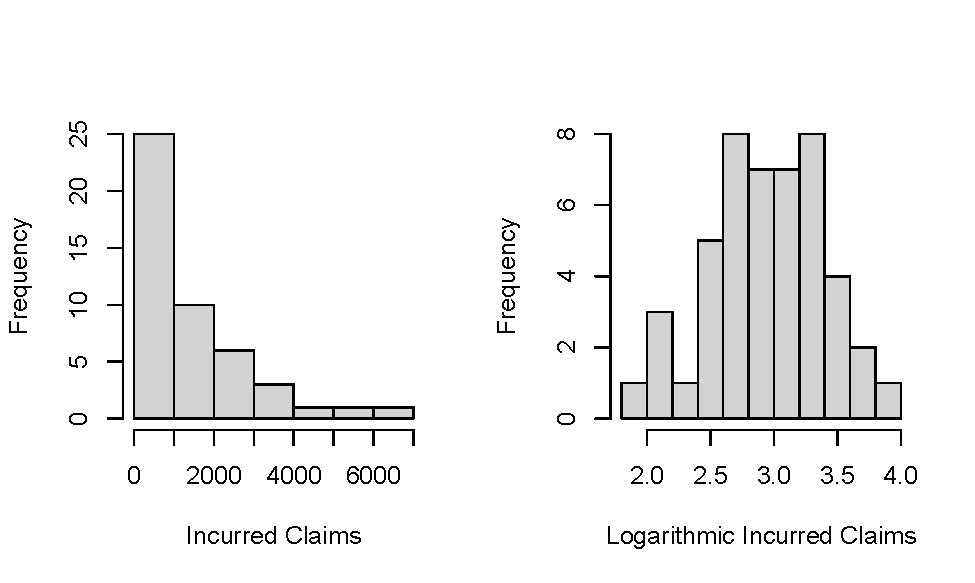
\includegraphics[width=0.8\linewidth]{LossDataAnalytics_files/figure-latex/GPAClaim1-1} 

}

\caption{\textbf{Distribution of Incurred Claims 2015-2019}}\label{fig:GPAClaim1}
\end{figure}

\emph{d.~Loss Distributions over Time.} There are 112 incurred losses. Figure \ref{fig:GPALossTime} indicates that the incurred losses are stable over the period 2015-2019, inclusive. Produce a comparable figure for the entire period and comment on the stability of the distribution.

\begin{figure}

{\centering 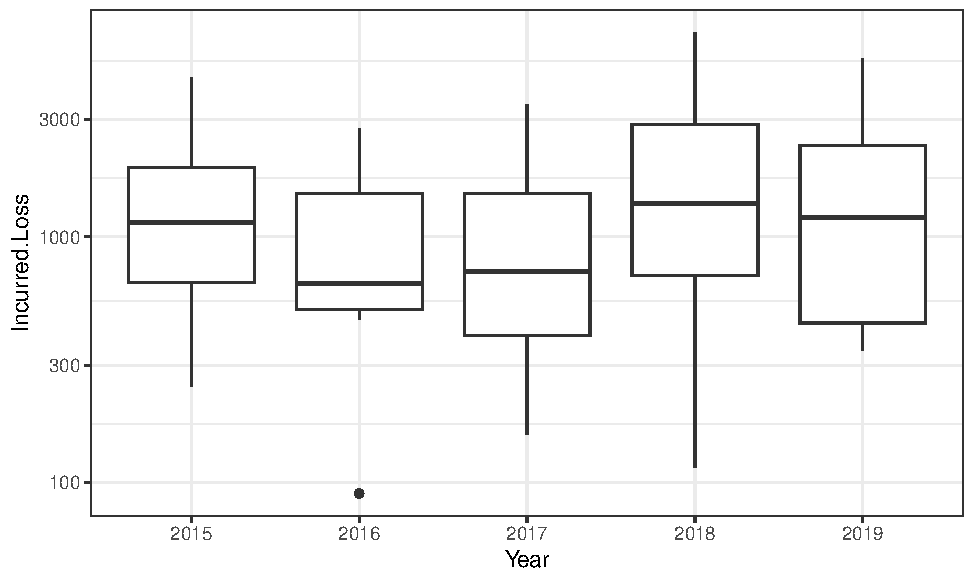
\includegraphics[width=0.7\linewidth]{LossDataAnalytics_files/figure-latex/GPALossTime-1} 

}

\caption{**Distribution of Group Personal Accident Losses by Year**}\label{fig:GPALossTime}
\end{figure}

\begin{Shaded}
\begin{Highlighting}[]
\CommentTok{\# a}
\NormalTok{GPAClaims }\OtherTok{\textless{}{-}} \FunctionTok{read.csv}\NormalTok{(}\StringTok{"Data/ANUGroupPersonalAccidentClaims2022.csv"}\NormalTok{, }\AttributeTok{header =}\NormalTok{ T)}
\NormalTok{GPAClaimsGT10 }\OtherTok{\textless{}{-}} \FunctionTok{subset}\NormalTok{(GPAClaims, Incurred.Loss }\SpecialCharTok{\textgreater{}=} \DecValTok{10}\NormalTok{)}
\NormalTok{tableGPAFreq }\OtherTok{\textless{}{-}} \FunctionTok{table}\NormalTok{(GPAClaimsGT10}\SpecialCharTok{$}\NormalTok{UW.Year)}
\NormalTok{knitr}\SpecialCharTok{::}\FunctionTok{kable}\NormalTok{(}\FunctionTok{t}\NormalTok{(tableGPAFreq), }\AttributeTok{align =} \StringTok{"cccccccc"}\NormalTok{, }\AttributeTok{caption =} \StringTok{"**Group Personal Accident Claims Frequency**"}\NormalTok{)}
\end{Highlighting}
\end{Shaded}

\begin{table}

\caption{\label{tab:unnamed-chunk-20}**Group Personal Accident Claims Frequency**}
\centering
\begin{tabular}[t]{c|c|c|c|c|c|c|c|c|c|c|c}
\hline
2010 & 2011 & 2012 & 2013 & 2014 & 2015 & 2016 & 2017 & 2018 & 2019 & 2020 & 2021\\
\hline
3 & 5 & 4 & 8 & 8 & 4 & 7 & 16 & 11 & 9 & 28 & 9\\
\hline
\end{tabular}
\end{table}

\begin{Shaded}
\begin{Highlighting}[]
\CommentTok{\# b}
\FunctionTok{par}\NormalTok{(}\AttributeTok{mfrow =} \FunctionTok{c}\NormalTok{(}\DecValTok{1}\NormalTok{, }\DecValTok{2}\NormalTok{))}
\FunctionTok{hist}\NormalTok{(GPAClaimsGT10}\SpecialCharTok{$}\NormalTok{Incurred.Loss, }\AttributeTok{main =} \StringTok{""}\NormalTok{, }\AttributeTok{xlab =} \StringTok{"Inclurred Claims"}\NormalTok{)}
\FunctionTok{hist}\NormalTok{(}\FunctionTok{log10}\NormalTok{(GPAClaimsGT10}\SpecialCharTok{$}\NormalTok{Incurred.Loss), }\AttributeTok{main =} \StringTok{""}\NormalTok{, }\AttributeTok{xlab =} \StringTok{"Logarithmic Incurred Claims"}\NormalTok{)}
\end{Highlighting}
\end{Shaded}

\begin{center}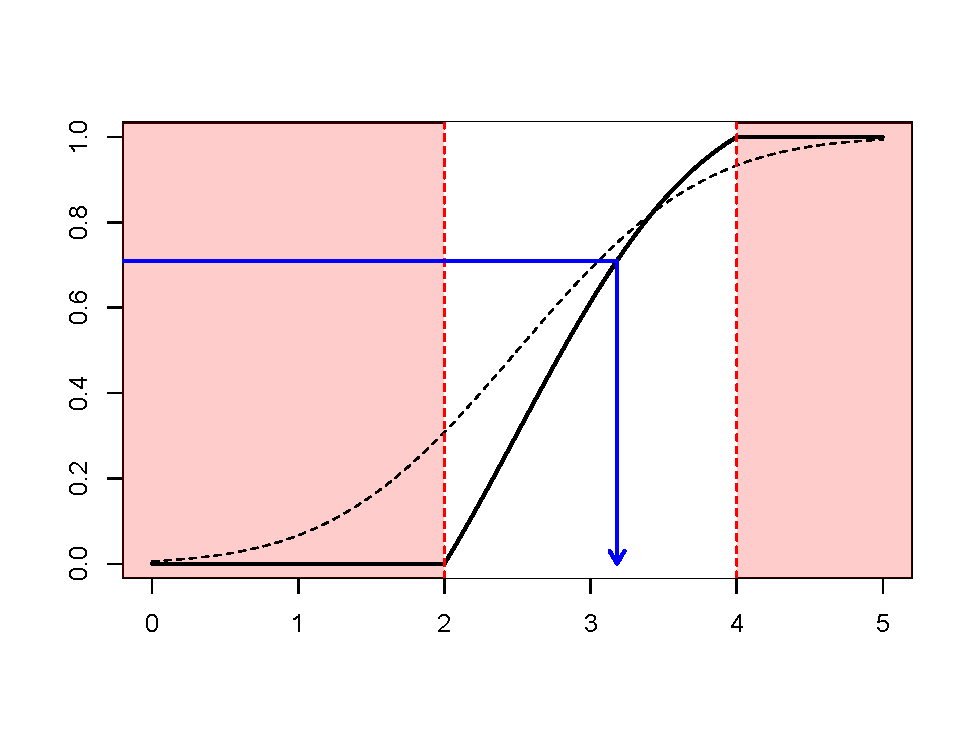
\includegraphics{LossDataAnalytics_files/figure-latex/unnamed-chunk-20-1} \end{center}

\begin{Shaded}
\begin{Highlighting}[]
\CommentTok{\# c}
\NormalTok{sumGPAClaimsGT10 }\OtherTok{\textless{}{-}} \FunctionTok{t}\NormalTok{(}\FunctionTok{summary}\NormalTok{(GPAClaimsGT10}\SpecialCharTok{$}\NormalTok{Incurred.Loss, }\AttributeTok{digits =} \DecValTok{0}\NormalTok{))}
\NormalTok{LogsumGPAClaimsGT10 }\OtherTok{\textless{}{-}} \FunctionTok{t}\NormalTok{(}\FunctionTok{summary}\NormalTok{(}\FunctionTok{log10}\NormalTok{(GPAClaimsGT10}\SpecialCharTok{$}\NormalTok{Incurred.Loss), }\AttributeTok{digits =} \DecValTok{4}\NormalTok{))}
\NormalTok{tabSumStats }\OtherTok{\textless{}{-}} \FunctionTok{rbind}\NormalTok{(sumGPAClaimsGT10, LogsumGPAClaimsGT10)}
\FunctionTok{rownames}\NormalTok{(tabSumStats) }\OtherTok{\textless{}{-}} \FunctionTok{c}\NormalTok{(}\StringTok{"Claims"}\NormalTok{, }\StringTok{"Log Claims"}\NormalTok{)}
\NormalTok{knitr}\SpecialCharTok{::}\FunctionTok{kable}\NormalTok{(tabSumStats, }\AttributeTok{align =} \StringTok{"cccccccc"}\NormalTok{, }\AttributeTok{caption =} \StringTok{"**Group Personal Accident Incurred Losses**"}\NormalTok{)}
\end{Highlighting}
\end{Shaded}

\begin{table}

\caption{\label{tab:unnamed-chunk-20}**Group Personal Accident Incurred Losses**}
\centering
\begin{tabular}[t]{l|c|c|c|c|c|c}
\hline
  & Min. & 1st Qu. & Median & Mean & 3rd Qu. & Max.\\
\hline
Claims & 90.000 & 500.000 & 1000 & 2000.000 & 2000.000 & 30000.000\\
\hline
Log Claims & 1.954 & 2.705 & 3 & 3.033 & 3.389 & 4.492\\
\hline
\end{tabular}
\end{table}

\begin{Shaded}
\begin{Highlighting}[]
\CommentTok{\# d}
\FunctionTok{ggplot}\NormalTok{(}\AttributeTok{data =}\NormalTok{ GPAClaimsGT10, }\FunctionTok{aes}\NormalTok{(}\AttributeTok{x =} \FunctionTok{factor}\NormalTok{(UW.Year), }\AttributeTok{y =}\NormalTok{ Incurred.Loss)) }\SpecialCharTok{+} \FunctionTok{geom\_boxplot}\NormalTok{() }\SpecialCharTok{+}
    \FunctionTok{theme\_bw}\NormalTok{() }\SpecialCharTok{+} \FunctionTok{xlab}\NormalTok{(}\StringTok{"Year"}\NormalTok{) }\SpecialCharTok{+} \FunctionTok{scale\_y\_continuous}\NormalTok{(}\AttributeTok{trans =} \StringTok{"log10"}\NormalTok{)}
\end{Highlighting}
\end{Shaded}

\begin{center}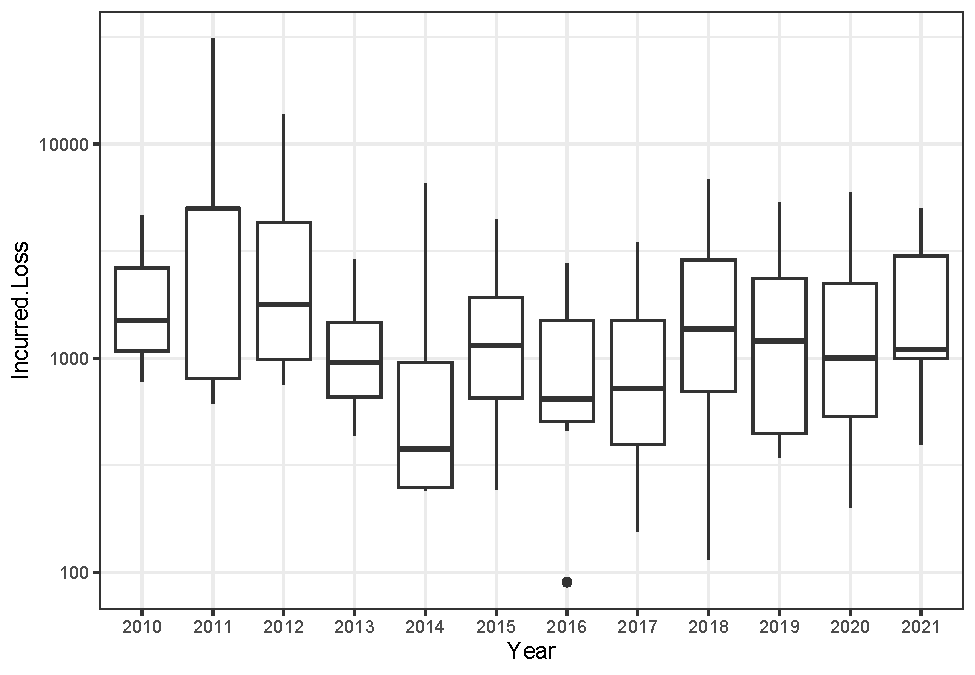
\includegraphics{LossDataAnalytics_files/figure-latex/unnamed-chunk-20-2} \end{center}

\begin{center}\rule{0.5\linewidth}{0.5pt}\end{center}

\textbf{Exercise 1.3. Motor Vehicle.} This policy covers ANU's vehicles including cars, vans, utilities, and motorcycles. There are two parts to this coverage, one for comprehensive damage to the insured vehicles and a second for legal liability. The comprehensive coverage for loss or damage is essentially limited by the market value of the insured vehicle. For legal liability, there is a \$50 Million upper limit for all claims arising from the one accident or series of accidents resulting from the one original cause. There is also another upper limit (that is lower than 50 million) when the vehicle is used for transportation of dangerous goods.

The data available contain the amount paid by the insurer (Vero Insurance Limited) which is the focus of our initial analysis. In addition, the data also contains a deductible (called an ``excess'' in the data file) that we explore in later parts.

The data provided to us are maintained by the insurer, Vero Insurance Limited. These data began in underwriting year 2012 and were accessed on 8 August 2022. You can retrieve the data by going to Appendix Section \ref{Sec:DataAuto}.

\emph{a. Adjust for Zeros.} From this data set, check that:

\begin{itemize}
\tightlist
\item
  there are 318 incurred claims.
\item
  Of these claims, there are 50 zeros and
\item
  an additional 0 claims where the incurred claim is less than 10.
\end{itemize}

Remove these claims in your analysis, so that there are 268 incurred claims.

\emph{b. Claim Frequency.} Produce a table that shows the count of claims for the entire period.

\emph{c.~Loss Distributions over Time.} Produce a figure that shows the distribution of motor vehicle paid amounts over time and comment on the stability of the distribution.

\emph{d.~Year 2019}. In your analysis from the prior steps, you may have noticed the unusual aspects of year 2019. In that year, ANU suffered extensive damage from a hailstorm that increased the frequency of claims as well as the severity. Produce a histogram of paid claims for that year.

\emph{e. Deductibles.} For each event, or series of events arising from the one originating cause, ANU bears the amount of the excess in respect of each and every insured vehicle, unless stated otherwise. The standard deductible (or excess) in the dataset is 1000. However, a cursory examination of the dataset shows tremendous variation by vehicle and over time.Replicate Table \ref{tab:TableExcess} that shows, for each year, the number of claims with zero excess, positive excess less than 1000, an excess equal to 1000, and an excess greater than 1000.

\begin{table}

\caption{\label{tab:TableExcess}**Motor Vehicle Excess by Year**}
\centering
\begin{tabular}[t]{c|c|c|c|c|c}
\hline
UW.Year & Num 0 & Num 0-1000 & Num = 1000 & Num >1000 & Total\\
\hline
2011 & 1 & 1 & 7 & 0 & 9\\
\hline
2012 & 1 & 2 & 13 & 0 & 16\\
\hline
2013 & 4 & 1 & 22 & 0 & 27\\
\hline
2014 & 0 & 0 & 11 & 0 & 11\\
\hline
2015 & 1 & 1 & 14 & 0 & 16\\
\hline
2016 & 6 & 1 & 19 & 0 & 26\\
\hline
2017 & 16 & 0 & 4 & 1 & 21\\
\hline
2018 & 19 & 0 & 1 & 0 & 20\\
\hline
2019 & 99 & 0 & 6 & 0 & 105\\
\hline
2020 & 5 & 0 & 0 & 0 & 5\\
\hline
2021 & 10 & 0 & 0 & 0 & 10\\
\hline
\end{tabular}
\end{table}

(\textbf{Deductibles}. We recommend that motivated readers extend our analysis to account for this deductible in both the severity and frequency.)

\begin{Shaded}
\begin{Highlighting}[]
\CommentTok{\# a}
\NormalTok{AutoClaims }\OtherTok{\textless{}{-}} \FunctionTok{read.csv}\NormalTok{(}\StringTok{"Data/ANUMotorClaims2022.csv"}\NormalTok{, }\AttributeTok{header =}\NormalTok{ T)}
\FunctionTok{length}\NormalTok{(AutoClaims}\SpecialCharTok{$}\NormalTok{Motor.Net.Incurred)  }\CommentTok{\# Number of incurred claims }
\end{Highlighting}
\end{Shaded}

\begin{verbatim}
[1] 318
\end{verbatim}

\begin{Shaded}
\begin{Highlighting}[]
\FunctionTok{sum}\NormalTok{(AutoClaims}\SpecialCharTok{$}\NormalTok{Motor.Net.Incurred }\SpecialCharTok{==} \DecValTok{0}\NormalTok{)  }\CommentTok{\# Number of zeros and }
\end{Highlighting}
\end{Shaded}

\begin{verbatim}
[1] 50
\end{verbatim}

\begin{Shaded}
\begin{Highlighting}[]
\FunctionTok{sum}\NormalTok{((AutoClaims}\SpecialCharTok{$}\NormalTok{Motor.Net.Incurred }\SpecialCharTok{\textgreater{}} \DecValTok{0}\NormalTok{) }\SpecialCharTok{*}\NormalTok{ (AutoClaims}\SpecialCharTok{$}\NormalTok{Motor.Net.Incurred }\SpecialCharTok{\textless{}} \DecValTok{10}\NormalTok{))  }\CommentTok{\# Number of incurred claims  where the incurred claim is less than 10. }
\end{Highlighting}
\end{Shaded}

\begin{verbatim}
[1] 0
\end{verbatim}

\begin{Shaded}
\begin{Highlighting}[]
\NormalTok{AutoClaimsGT10 }\OtherTok{\textless{}{-}} \FunctionTok{subset}\NormalTok{(AutoClaims, Motor.Net.Incurred }\SpecialCharTok{\textgreater{}=} \DecValTok{10}\NormalTok{)}
\FunctionTok{length}\NormalTok{(AutoClaimsGT10}\SpecialCharTok{$}\NormalTok{Motor.Net.Incurred)  }\CommentTok{\# length of the smaller dataset}
\end{Highlighting}
\end{Shaded}

\begin{verbatim}
[1] 268
\end{verbatim}

\begin{Shaded}
\begin{Highlighting}[]
\CommentTok{\# b}
\NormalTok{UwYear }\OtherTok{\textless{}{-}} \FunctionTok{as.Date}\NormalTok{(AutoClaimsGT10}\SpecialCharTok{$}\NormalTok{Policy.Term.Start.Date, }\StringTok{"\%d/\%m/\%Y"}\NormalTok{)}
\NormalTok{AutoClaimsGT10}\SpecialCharTok{$}\NormalTok{UW.Year }\OtherTok{\textless{}{-}} \FunctionTok{as.numeric}\NormalTok{(}\FunctionTok{format}\NormalTok{(UwYear, }\AttributeTok{format =} \StringTok{"\%Y"}\NormalTok{))}
\NormalTok{tableAutoClaims }\OtherTok{\textless{}{-}} \FunctionTok{t}\NormalTok{(}\FunctionTok{table}\NormalTok{(AutoClaimsGT10}\SpecialCharTok{$}\NormalTok{UW.Year))}
\NormalTok{knitr}\SpecialCharTok{::}\FunctionTok{kable}\NormalTok{(tableAutoClaims, }\AttributeTok{align =} \StringTok{"cccccccc"}\NormalTok{, }\AttributeTok{caption =} \StringTok{"**Motor Vehicle Claim Frequency**"}\NormalTok{)}
\end{Highlighting}
\end{Shaded}

\begin{table}

\caption{\label{tab:unnamed-chunk-22}**Motor Vehicle Claim Frequency**}
\centering
\begin{tabular}[t]{c|c|c|c|c|c|c|c|c|c|c}
\hline
2011 & 2012 & 2013 & 2014 & 2015 & 2016 & 2017 & 2018 & 2019 & 2020 & 2021\\
\hline
10 & 17 & 27 & 11 & 16 & 26 & 21 & 20 & 105 & 5 & 10\\
\hline
\end{tabular}
\end{table}

\begin{Shaded}
\begin{Highlighting}[]
\CommentTok{\# c}
\FunctionTok{ggplot}\NormalTok{(}\AttributeTok{data =}\NormalTok{ AutoClaimsGT10, }\FunctionTok{aes}\NormalTok{(}\AttributeTok{x =} \FunctionTok{factor}\NormalTok{(UW.Year), }\AttributeTok{y =}\NormalTok{ Motor.Net.Incurred)) }\SpecialCharTok{+}
    \FunctionTok{geom\_boxplot}\NormalTok{() }\SpecialCharTok{+} \FunctionTok{theme\_bw}\NormalTok{() }\SpecialCharTok{+} \FunctionTok{xlab}\NormalTok{(}\StringTok{"Year"}\NormalTok{) }\SpecialCharTok{+} \FunctionTok{scale\_y\_continuous}\NormalTok{(}\AttributeTok{trans =} \StringTok{"log10"}\NormalTok{)}
\end{Highlighting}
\end{Shaded}

\begin{center}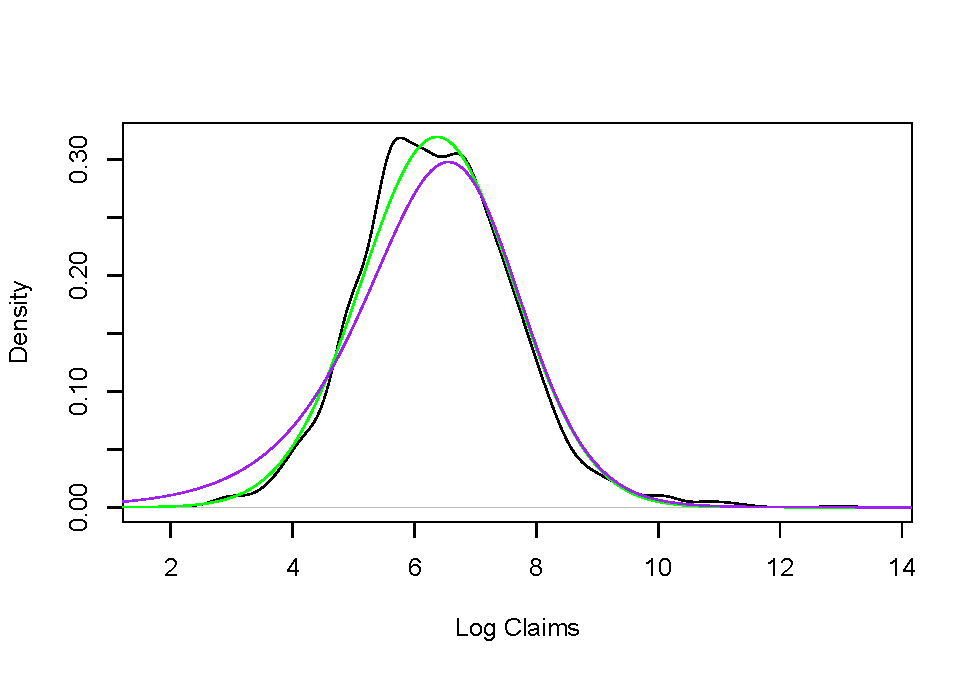
\includegraphics[width=0.7\linewidth]{LossDataAnalytics_files/figure-latex/unnamed-chunk-22-1} \end{center}

\begin{Shaded}
\begin{Highlighting}[]
\CommentTok{\# d}
\NormalTok{AutoClaims2019 }\OtherTok{\textless{}{-}} \FunctionTok{subset}\NormalTok{(AutoClaimsGT10, UW.Year }\SpecialCharTok{==} \DecValTok{2019}\NormalTok{)}
\FunctionTok{hist}\NormalTok{(AutoClaims2019}\SpecialCharTok{$}\NormalTok{Motor.Net.Incurred, }\AttributeTok{main =} \StringTok{""}\NormalTok{, }\AttributeTok{xlab =} \StringTok{"2019 Motor Vehicle Claims"}\NormalTok{)}
\end{Highlighting}
\end{Shaded}

\begin{center}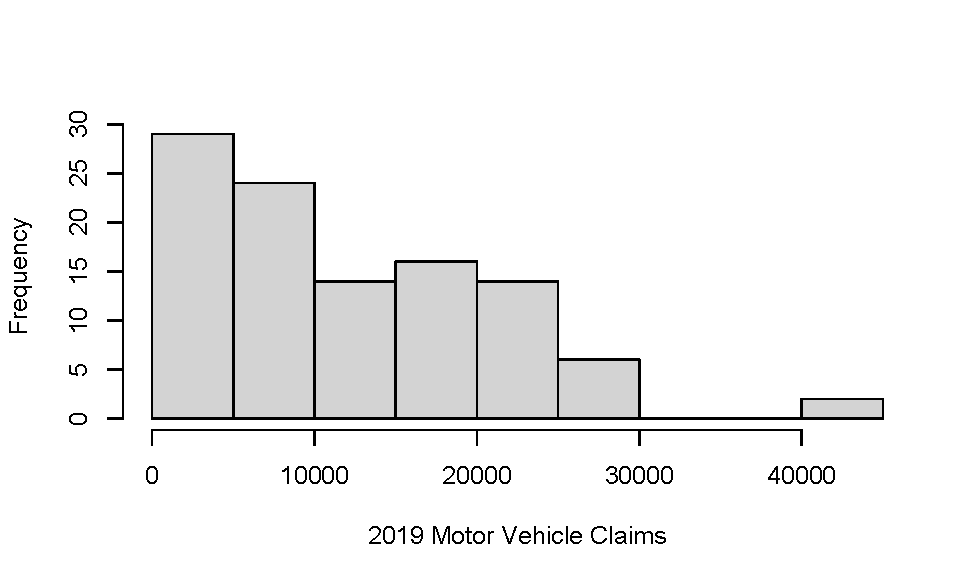
\includegraphics[width=0.7\linewidth]{LossDataAnalytics_files/figure-latex/unnamed-chunk-22-2} \end{center}

\begin{Shaded}
\begin{Highlighting}[]
\CommentTok{\# e}
\NormalTok{AutoClaimsGT10}\SpecialCharTok{$}\NormalTok{Excess0 }\OtherTok{\textless{}{-}} \DecValTok{1} \SpecialCharTok{*}\NormalTok{ (AutoClaimsGT10}\SpecialCharTok{$}\NormalTok{Excess }\SpecialCharTok{==} \DecValTok{0}\NormalTok{)}
\NormalTok{AutoClaimsGT10}\SpecialCharTok{$}\NormalTok{ExcessLT1000 }\OtherTok{\textless{}{-}} \DecValTok{1} \SpecialCharTok{*}\NormalTok{ (AutoClaimsGT10}\SpecialCharTok{$}\NormalTok{Excess }\SpecialCharTok{\textless{}} \DecValTok{1000}\NormalTok{) }\SpecialCharTok{*}\NormalTok{ (AutoClaimsGT10}\SpecialCharTok{$}\NormalTok{Excess }\SpecialCharTok{\textgreater{}}
    \DecValTok{0}\NormalTok{)}
\NormalTok{AutoClaimsGT10}\SpecialCharTok{$}\NormalTok{ExcessEq1000 }\OtherTok{\textless{}{-}} \DecValTok{1} \SpecialCharTok{*}\NormalTok{ (AutoClaimsGT10}\SpecialCharTok{$}\NormalTok{Excess }\SpecialCharTok{==} \DecValTok{1000}\NormalTok{)}
\NormalTok{AutoClaimsGT10}\SpecialCharTok{$}\NormalTok{ExcessGT1000 }\OtherTok{\textless{}{-}} \DecValTok{1} \SpecialCharTok{*}\NormalTok{ (AutoClaimsGT10}\SpecialCharTok{$}\NormalTok{Excess }\SpecialCharTok{\textgreater{}} \DecValTok{1000}\NormalTok{)}
\NormalTok{AutoClaimsGT10}\SpecialCharTok{$}\NormalTok{Constant1 }\OtherTok{\textless{}{-}}\NormalTok{ AutoClaimsGT10}\SpecialCharTok{$}\NormalTok{Excess0 }\SpecialCharTok{*} \DecValTok{0} \SpecialCharTok{+} \DecValTok{1}
\FunctionTok{library}\NormalTok{(doBy)}
\NormalTok{T1 }\OtherTok{\textless{}{-}} \FunctionTok{summaryBy}\NormalTok{(Excess0 }\SpecialCharTok{\textasciitilde{}}\NormalTok{ UW.Year, }\AttributeTok{data =}\NormalTok{ AutoClaimsGT10, }\AttributeTok{FUN =} \ControlFlowTok{function}\NormalTok{(x) \{}
\NormalTok{    m }\OtherTok{=} \FunctionTok{sum}\NormalTok{(x, }\AttributeTok{na.rm =} \ConstantTok{TRUE}\NormalTok{)}
\NormalTok{\})}
\NormalTok{T2 }\OtherTok{\textless{}{-}} \FunctionTok{summaryBy}\NormalTok{(ExcessLT1000 }\SpecialCharTok{\textasciitilde{}}\NormalTok{ UW.Year, }\AttributeTok{data =}\NormalTok{ AutoClaimsGT10, }\AttributeTok{FUN =} \ControlFlowTok{function}\NormalTok{(x) \{}
\NormalTok{    m }\OtherTok{=} \FunctionTok{sum}\NormalTok{(x, }\AttributeTok{na.rm =} \ConstantTok{TRUE}\NormalTok{)}
\NormalTok{\})}
\NormalTok{T3 }\OtherTok{\textless{}{-}} \FunctionTok{summaryBy}\NormalTok{(ExcessEq1000 }\SpecialCharTok{\textasciitilde{}}\NormalTok{ UW.Year, }\AttributeTok{data =}\NormalTok{ AutoClaimsGT10, }\AttributeTok{FUN =} \ControlFlowTok{function}\NormalTok{(x) \{}
\NormalTok{    m }\OtherTok{=} \FunctionTok{sum}\NormalTok{(x, }\AttributeTok{na.rm =} \ConstantTok{TRUE}\NormalTok{)}
\NormalTok{\})}
\NormalTok{T4 }\OtherTok{\textless{}{-}} \FunctionTok{summaryBy}\NormalTok{(ExcessGT1000 }\SpecialCharTok{\textasciitilde{}}\NormalTok{ UW.Year, }\AttributeTok{data =}\NormalTok{ AutoClaimsGT10, }\AttributeTok{FUN =} \ControlFlowTok{function}\NormalTok{(x) \{}
\NormalTok{    m }\OtherTok{=} \FunctionTok{sum}\NormalTok{(x, }\AttributeTok{na.rm =} \ConstantTok{TRUE}\NormalTok{)}
\NormalTok{\})}
\NormalTok{T5 }\OtherTok{\textless{}{-}} \FunctionTok{summaryBy}\NormalTok{(Constant1 }\SpecialCharTok{\textasciitilde{}}\NormalTok{ UW.Year, }\AttributeTok{data =}\NormalTok{ AutoClaimsGT10, }\AttributeTok{FUN =} \ControlFlowTok{function}\NormalTok{(x) \{}
\NormalTok{    m }\OtherTok{=} \FunctionTok{sum}\NormalTok{(x, }\AttributeTok{na.rm =} \ConstantTok{TRUE}\NormalTok{)}
\NormalTok{\})}
\NormalTok{TableOut }\OtherTok{\textless{}{-}} \FunctionTok{cbind}\NormalTok{(T1, T2[}\DecValTok{2}\NormalTok{], T3[}\DecValTok{2}\NormalTok{], T4[}\DecValTok{2}\NormalTok{], T5[}\DecValTok{2}\NormalTok{])}
\FunctionTok{colnames}\NormalTok{(TableOut) }\OtherTok{\textless{}{-}} \FunctionTok{c}\NormalTok{(}\StringTok{"UW.Year"}\NormalTok{, }\StringTok{"Num 0"}\NormalTok{, }\StringTok{"Num 0{-}1000"}\NormalTok{, }\StringTok{"Num = 1000"}\NormalTok{, }\StringTok{"Num \textgreater{}1000"}\NormalTok{,}
    \StringTok{"Total"}\NormalTok{)}

\NormalTok{knitr}\SpecialCharTok{::}\FunctionTok{kable}\NormalTok{(TableOut, }\AttributeTok{align =} \StringTok{"cccccccc"}\NormalTok{, }\AttributeTok{caption =} \StringTok{"**Motor Vehicle Excess by Year**"}\NormalTok{)}
\end{Highlighting}
\end{Shaded}

\begin{table}

\caption{\label{tab:unnamed-chunk-22}**Motor Vehicle Excess by Year**}
\centering
\begin{tabular}[t]{c|c|c|c|c|c}
\hline
UW.Year & Num 0 & Num 0-1000 & Num = 1000 & Num >1000 & Total\\
\hline
2011 & 1 & 1 & 7 & 0 & 9\\
\hline
2012 & 1 & 2 & 13 & 0 & 16\\
\hline
2013 & 4 & 1 & 22 & 0 & 27\\
\hline
2014 & 0 & 0 & 11 & 0 & 11\\
\hline
2015 & 1 & 1 & 14 & 0 & 16\\
\hline
2016 & 6 & 1 & 19 & 0 & 26\\
\hline
2017 & 16 & 0 & 4 & 1 & 21\\
\hline
2018 & 19 & 0 & 1 & 0 & 20\\
\hline
2019 & 99 & 0 & 6 & 0 & 105\\
\hline
2020 & 5 & 0 & 0 & 0 & 5\\
\hline
2021 & 10 & 0 & 0 & 0 & 10\\
\hline
\end{tabular}
\end{table}

\begin{center}\rule{0.5\linewidth}{0.5pt}\end{center}

We provide summaries of this information simply so that readers can see what type of data are available for more in-depth analysis. Specifically, in addition to incurred losses, we also have the following information

\begin{Shaded}
\begin{Highlighting}[]
\NormalTok{knitr}\SpecialCharTok{::}\FunctionTok{kable}\NormalTok{(}\FunctionTok{summary}\NormalTok{(AutoClaims)[, }\SpecialCharTok{{-}}\DecValTok{1}\NormalTok{])}
\end{Highlighting}
\end{Shaded}

\begin{tabular}{l|l|l|l|l|l|l|l|l|l|l|l|l}
\hline
  &  Loss.Date & Reported.Date & Motor.Fault &   Driver.Age & Vehicle.Description & Loss.Postcode &     Excess & Motor.Net.Paid & Outstanding.Estimate & Motor.Net.Incurred & Third.Party.Identified & Third.Party.Insured\\
\hline
 & Length:318 & Length:318 & Length:318 & Min.   :18.00 & Length:318 & Min.   : 200 & Min.   :   0.0 & Min.   :    0.0 & Min.   :    0.0 & Min.   :    0.0 & Length:318 & Length:318\\
\hline
 & Class :character & Class :character & Class :character & 1st Qu.:28.00 & Class :character & 1st Qu.:2559 & 1st Qu.:   0.0 & 1st Qu.:  315.6 & 1st Qu.:    0.0 & 1st Qu.:  385.2 & Class :character & Class :character\\
\hline
 & Mode  :character & Mode  :character & Mode  :character & Median :40.00 & Mode  :character & Median :2601 & Median :   0.0 & Median : 1787.8 & Median :    0.0 & Median : 1894.7 & Mode  :character & Mode  :character\\
\hline
 & NA & NA & NA & Mean   :41.26 & NA & Mean   :2669 & Mean   : 337.3 & Mean   : 5299.6 & Mean   :  199.2 & Mean   : 5498.8 & NA & NA\\
\hline
 & NA & NA & NA & 3rd Qu.:55.00 & NA & 3rd Qu.:2609 & 3rd Qu.:1000.0 & 3rd Qu.: 6804.1 & 3rd Qu.:    0.0 & 3rd Qu.: 7013.1 & NA & NA\\
\hline
 & NA & NA & NA & Max.   :69.00 & NA & Max.   :7320 & Max.   :2000.0 & Max.   :56469.6 & Max.   :31927.3 & Max.   :56469.6 & NA & NA\\
\hline
 & NA & NA & NA & NA's   :145 & NA & NA's   :3 & NA's   :2 & NA & NA & NA & NA & NA\\
\hline
\end{tabular}

\begin{Shaded}
\begin{Highlighting}[]
\CommentTok{\# \%\textgreater{}\% kableExtra::kable\_classic(font = 8, html\_font = \textquotesingle{}Cambria\textquotesingle{})}
\end{Highlighting}
\end{Shaded}

\begin{center}\rule{0.5\linewidth}{0.5pt}\end{center}

\hypertarget{Intro-further-reading-and-resources}{%
\section{Further Resources and Contributors}\label{Intro-further-reading-and-resources}}

\hypertarget{contributor}{%
\subsubsection*{Contributor}\label{contributor}}
\addcontentsline{toc}{subsubsection}{Contributor}

\begin{itemize}
\tightlist
\item
  \textbf{Edward (Jed) Frees}, University of Wisconsin-Madison, is the principal author of the initial version of this chapter.
\item
  Chapter reviewers include: Yair Babad, Chunsheng Ban, Aaron Bruhn, Gordon Enderle, Hirokazu (Iwahiro) Iwasawa, Dalia Khalil, Bell Ouelega, Michelle Xia.
\item
  \textbf{Edward (Jed) Frees}, University of Wisconsin-Madison and Australian National University, is the author of the second edition of this chapter. Email: \href{mailto:jfrees@bus.wisc.edu}{\nolinkurl{jfrees@bus.wisc.edu}} for chapter comments and suggested improvements.
\end{itemize}

This book introduces loss data analytic tools that are most relevant to actuaries and other financial risk analysts. We have also introduced you to many new insurance terms; more terms can be found at the \citet{NAICGlossary}. Here are a few references cited in the chapter.

\begin{center}\rule{0.5\linewidth}{0.5pt}\end{center}

This work is licensed under a Creative Commons Attribution 4.0 International License.

\hypertarget{DataResources}{%
\chapter{Appendix. Data Resources}\label{DataResources}}

This appendix section describes the datasets used in this book and others that you may wish to explore.

For each set of data, we provide download buttons so that you can easily access the data in standard .csv (comma separated value) format. This allows you replicate and experiment with the methods developed in the book as well as sharpen your understanding through exercises.

We provide the source of each dataset. We also recommend, for deeper understanding, that you occasionally refer to these original sources to further develop your appreciation of the data underpinning the analytics developed in this book.

\hypertarget{S:WiscPropFundA}{%
\section{Wisconsin Property Fund}\label{S:WiscPropFundA}}

\textbf{Description}: The Wisconsin Local Government Property Insurance Fund (LGPIF) is an insurance pool administered by the Wisconsin Office of the Insurance Commissioner. The LGPIF was established to provide property insurance for local government entities that include counties, cities, towns, villages, school districts, and library boards. The fund insures local government property such as government buildings, schools, libraries, and motor vehicles. It covers all property losses except those resulting from flood, earthquake, wear and tear, extremes in temperature, mold, war, nuclear reactions, and embezzlement or theft by an employee.

The data are available using this download button:
Download the Wisconsin Property Fund Data

\begin{table}

\caption{\label{tab:unnamed-chunk-27}**Variables in the Wisconsin Property Fund Dataset**}
\centering
\begin{tabular}[t]{ll}
\toprule
Variable & Description\\
\midrule
PolicyNum & Policy number\\
Year & Contract year\\
Premium & Premium\\
Deduct & Deductible\\
BCcov & Coverage for building and contents\\
\addlinespace
Freq & Number of claims during the year (frequency)\\
Fire5 & Binary variable to indicate the fire class is below 5\\
NoClaimCredit & Binary variable to indicate no claims in the past two years\\
EntityType & Categorical variable that is one of six types:  1=Village, 2=City,3=County, 4=Misc, 5=School, or Town)\\
AlarmCredit & Categorical variable that is one of four types:  (0, 5, 10, or 15) for automatic smoke alarms in main rooms\\
\addlinespace
BCClaim & Builing and contents claims\\
\bottomrule
\end{tabular}
\end{table}

\begin{table}

\caption{\label{tab:unnamed-chunk-28}**Wisconsin Property Fund First Five Rows**}
\centering
\begin{tabular}[t]{c|c|c|c|c|c|c|c|c|c|c}
\hline
PolicyNum & Year & Premium & Deduct & BCcov & Freq & Fire5 & NoClaimCredit & EntityType & AlarmCredit & BCClaim\\
\hline
120002 & 2006 & 9313 & 1000 & 22714456 & 0 & 1 & 0 & 3 & 1 & 0.00\\
\hline
120002 & 2007 & 8767 & 1000 & 25046646 & 0 & 1 & 0 & 3 & 1 & 0.00\\
\hline
120002 & 2008 & 7090 & 1000 & 20851525 & 0 & 1 & 1 & 3 & 1 & 0.00\\
\hline
120002 & 2009 & 8522 & 1000 & 21852696 & 0 & 1 & 1 & 3 & 1 & 0.00\\
\hline
120002 & 2010 & 7994 & 1000 & 23511493 & 1 & 1 & 1 & 3 & 1 & 6838.87\\
\hline
\end{tabular}
\end{table}

\begin{table}

\caption{\label{tab:unnamed-chunk-28}**Wisconsin Property Fund Last Five Rows**}
\centering
\begin{tabular}[t]{c|c|c|c|c|c|c|c|c|c|c}
\hline
PolicyNum & Year & Premium & Deduct & BCcov & Freq & Fire5 & NoClaimCredit & EntityType & AlarmCredit & BCClaim\\
\hline
180787 & 2010 & 199 & 5e+02 & 285000 & 0 & 1 & 1 & 4 & 1 & 0.00\\
\hline
180788 & 2010 & 58344 & 1e+05 & 416739800 & 1 & 1 & 0 & 4 & 1 & 168304.05\\
\hline
180789 & 2010 & 295 & 5e+02 & 500988 & 1 & 1 & 0 & 4 & 1 & 1034.33\\
\hline
180790 & 2010 & 2077 & 1e+03 & 3580665 & 0 & 1 & 0 & 4 & 4 & 0.00\\
\hline
180791 & 2010 & 81 & 5e+02 & 118800 & 0 & 1 & 0 & 4 & 1 & 0.00\\
\hline
\end{tabular}
\end{table}

\hypertarget{Sec:DataTravel}{%
\section{ANU Corporate Travel Data}\label{Sec:DataTravel}}

Universities purchase corporate travel policies to cover employees and students traveling on official university business for a wide variety of accidents and incidents while away from the campus or primary workplace. This broad coverage includes medical care and evacuation, loss of personal property, extraction for political and weather related reasons, and more. See \citet{frees2022ANURisks} for more information about this coverage.

There are 2107 observations in this dataset. The variable names are described in Table \ref{tab:DescribeTravel} and the first and last five observations are in Table \ref{tab:PrintNumTravel}.

Data are available using this button:
Download Corporate Travel Claims Data.

\begin{table}

\caption{\label{tab:DescribeTravel}**Variables in the Corporate Travel Dataset**}
\centering
\begin{tabular}[t]{ll}
\toprule
Variable & Description\\
\midrule
UW Year & Underwriting Year\\
Loss Date & Date that the loss occurred\\
Reported Date & Date that the loss was reported\\
Last Trans Date & Last date in which there was a transaction regarding the loss\\
Paid Loss & Cumulative amount paid on the loss\\
\addlinespace
Outstanding Reserve & Estimate of the loss amount yet to be paid\\
Incurred Loss & Sum of the amount paid and the estimate of future payments\\
Status & An indicator as to whether the claim has been deemed settled (closed) or not settled (open)\\
\bottomrule
\end{tabular}
\end{table}

\begin{table}

\caption{\label{tab:PrintNumTravel}**Corporate Travel Data First Five Rows**}
\centering
\begin{tabular}[t]{c|c|c|c|c|c|c|c}
\hline
UW.Year & Loss.Date & Reported.Date & Last.Trans.Date & Paid.Loss & Outstanding.Reserve & Incurred.Loss & Status\\
\hline
2021 & 19/12/2021 & 20/12/2021 & 24/12/2021 & 10000.00 & 0 & 10000.00 & Closed\\
\hline
2021 & 9/4/2022 & 29/04/2022 & 30/05/2022 & 423.08 & 0 & 423.08 & Closed\\
\hline
2021 & 2/5/2022 & 4/5/2022 &  & 0.00 & 500 & 500.00 & Open\\
\hline
2021 & 5/5/2022 & 17/05/2022 &  & 0.00 & 562 & 562.00 & Open\\
\hline
2021 & 30/04/2022 & 27/05/2022 & 10/6/2022 & 1500.00 & 0 & 1500.00 & Closed\\
\hline
\end{tabular}
\end{table}

\begin{table}

\caption{\label{tab:PrintNumTravel}**Corporate Travel Data Last Five Rows**}
\centering
\begin{tabular}[t]{c|c|c|c|c|c|c|c}
\hline
UW.Year & Loss.Date & Reported.Date & Last.Trans.Date & Paid.Loss & Outstanding.Reserve & Incurred.Loss & Status\\
\hline
2006 & 1/11/2006 & 19/06/2007 &  & 0.00 & 0 & 0.00 & Closed\\
\hline
2006 & 24/06/2007 & 26/06/2007 & 8/1/2008 & 6278.10 & 0 & 6278.10 & Closed\\
\hline
2006 & 4/7/2007 & 6/7/2007 & 11/9/2007 & 114.50 & 0 & 114.50 & Closed\\
\hline
2006 & 20/05/2007 & 26/06/2007 & 14/07/2007 & 135.65 & 0 & 135.65 & Closed\\
\hline
2006 & 15/02/2007 & 27/06/2007 & 14/07/2007 & 1207.75 & 0 & 1207.75 & Closed\\
\hline
\end{tabular}
\end{table}

\emph{Source}: Frees, Edward and Butt, Adam (2022). ``ANU Corporate Travel Insurance Claims 2022''. Australian National University Data Commons. DOI \url{https://doi.org/10.25911/vrdw-9f32}.

\hypertarget{Sec:DataGPA}{%
\section{ANU Group Personal Accident Data}\label{Sec:DataGPA}}

Group personal accident insurance offers financial protection in case of injury or death resulting from an incident that occurs on the job. Like workers' compensation, group personal accident offers insurance coverage and liability insurance protection against accidental death or injury. Unlike workers' compensation, group personal accident covers students and ANU's voluntary workers. See \citet{frees2022ANURisks} for more information about this coverage.

There are 148 observations in this dataset. The variable names are described in Table \ref{tab:DescribeGPA} and the first and last five observations are in Table \ref{tab:PrintNumGPA}.

Data are available using this button: Download Group Personal Accident Claims Data.

\begin{table}

\caption{\label{tab:DescribeGPA}**Variables in the Group Personal Accident Dataset**}
\centering
\begin{tabular}[t]{ll}
\toprule
Variable & Description\\
\midrule
UW Year & Underwriting Year\\
Loss Date & Date that the loss occurred\\
Last Trans Date & Last date in which there was a transaction regarding the loss.\\
Paid Loss & Cumulative amount paid on the loss\\
Outstanding Reserve & Estimate of the loss amount yet to be paid\\
\addlinespace
Incurred Loss & Sum of the amount paid and the estimate of future payments\\
Status & An indicator as to whether the claim has been deemed settled (closed) or not settled (open)\\
\bottomrule
\end{tabular}
\end{table}

\begin{table}

\caption{\label{tab:PrintNumGPA}**Group Personal Accident  Data First Five Rows**}
\centering
\begin{tabular}[t]{c|c|c|c|c|c|c}
\hline
UW.Year & Loss.Date & Last.Trans.Date & Paid.Loss & Outstanding.Reserve & Incurred.Loss & Status\\
\hline
2021 & 6/12/2021 & 3/6/2022 & 805.0 & 0.0 & 805 & Closed\\
\hline
2021 & 15/11/2021 &  & 0.0 & 0.0 & 0 & Closed\\
\hline
2021 & 15/11/2021 &  & 0.0 & 0.0 & 0 & Closed\\
\hline
2021 & 22/03/2022 & 4/5/2022 & 396.0 & 0.0 & 396 & Closed\\
\hline
2021 & 11/4/2022 & 2/8/2022 & 740.1 & 359.9 & 1100 & Open\\
\hline
\end{tabular}
\end{table}

\begin{table}

\caption{\label{tab:PrintNumGPA}**Group Personal Accident Data Last Five Rows**}
\centering
\begin{tabular}[t]{c|c|c|c|c|c|c}
\hline
UW.Year & Loss.Date & Last.Trans.Date & Paid.Loss & Outstanding.Reserve & Incurred.Loss & Status\\
\hline
2010 & 6/3/2011 & 26/07/2011 & 776.00 & 0 & 776.00 & Closed\\
\hline
2010 & 22/07/2011 & 23/01/2012 & 4624.54 & 0 & 4624.54 & Closed\\
\hline
2010 & 5/6/2011 & 30/01/2012 & 1503.65 & 0 & 1503.65 & Closed\\
\hline
2007 & 11/1/2008 & 23/02/2008 & 0.00 & 0 & 0.00 & Closed\\
\hline
2007 & 29/08/2008 &  & 0.00 & 0 & 0.00 & Closed\\
\hline
\end{tabular}
\end{table}

\emph{Source}: Frees, Edward and Butt, Adam (2022). ``ANU Group Personal Accident Claims 2022''. Australian National University Data Commons. \url{https://doi.org/10.25911/jcfx-zj56}.

\hypertarget{Sec:DataAuto}{%
\section{ANU Motor Vehicle Data}\label{Sec:DataAuto}}

This policy covers ANU's vehicles including cars, vans, utilities, and motorcycles. See \citet{frees2022ANURisks} for more information about this coverage.

There are 318 observations in this dataset. The variable names are described in Table \ref{tab:DescribeAuto} and the first and last five observations are in Table \ref{tab:PrintNumAuto}.

Data are available using this button:
Download Motor Vehicle Claims Data.

\begin{table}

\caption{\label{tab:DescribeAuto}**Variables in the Motor Vehicle Dataset**}
\centering
\begin{tabular}[t]{ll}
\toprule
Variable & Description\\
\midrule
Policy Term Start Date & Start date of the contract year in which the loss occurred\\
Loss Date & Date that the loss occurred\\
Reported Date & Date that the loss was reported\\
Motor Fault & Party responsible for the loss\\
Driver Age & Age of the driver\\
\addlinespace
Vehicle Description & Type of vehicle\\
Loss Postcode & Postal code where the loss occurred\\
Excess & The deductible applied to the loss\\
Motor Net Paid & Amount paid to the insured (ANU)\\
Outstanding Estimate & Estimate of the loss amount yet to be paid\\
\addlinespace
Motor Net Incurred & Sum of the amount paid and the estimate of future payments\\
Third Party Identified & Indicates whether a responsible third party could be identified\\
Third Party Insured & Indicates whether a responsible third party was insured\\
\bottomrule
\end{tabular}
\end{table}

\begin{table}

\caption{\label{tab:PrintNumAuto}**Motor Vehicle  Data First Five Rows**}
\centering
\begin{tabular}[t]{c|c|c|c|c|c|c}
\hline
Policy.Term.Start.Date & Loss.Date & Reported.Date & Motor.Fault & Driver.Age & Vehicle.Description & Loss.Postcode\\
\hline
1/11/2011 & 6/6/2012 & 4/10/2012 & THIRD PARTY RESPONSIBLE & NA & FORD TRANSIT VAN & 2600\\
\hline
1/11/2011 & 16/08/2012 & 14/11/2013 & INSURED RESPONSIBLE & 39 & TOYOTA HIACE & 2612\\
\hline
1/11/2011 & 4/9/2012 & 17/01/2013 & INSURED RESPONSIBLE & 52 & HYUNDAI IX35 & 2600\\
\hline
1/11/2011 & 21/09/2012 & 28/09/2012 & THIRD PARTY RESPONSIBLE & 59 & HOLDEN COMMODORE & 2518\\
\hline
1/11/2011 & 22/09/2012 & 12/10/2012 & INSURED RESPONSIBLE & NA & SUBARU FORESTER & 2612\\
\hline
\end{tabular}
\end{table}

\begin{tabular}{c|c|c|c|c|c}
\hline
Excess & Motor.Net.Paid & Outstanding.Estimate & Motor.Net.Incurred & Third.Party.Identified & Third.Party.Insured\\
\hline
1000 & 384.88 & 0 & 384.88 & IDENTIFIED & \\
\hline
1000 & 901.21 & 0 & 901.21 &  & \\
\hline
1000 & 1225.71 & 0 & 1225.71 &  & \\
\hline
NA & 1671.76 & 0 & 1671.76 & IDENTIFIED & NOT INSURED\\
\hline
1000 & 3418.86 & 0 & 3418.86 &  & INSURED\\
\hline
\end{tabular}

\begin{table}

\caption{\label{tab:PrintNumAuto}**Motor Vehicle Data Last Five Rows**}
\centering
\begin{tabular}[t]{c|c|c|c|c|c|c}
\hline
Policy.Term.Start.Date & Loss.Date & Reported.Date & Motor.Fault & Driver.Age & Vehicle.Description & Loss.Postcode\\
\hline
1/11/2021 & 4/4/2022 & 5/4/2022 & INSURED RESPONSIBLE & 66 & VOLKSWAGEN TIGUAN & 2604\\
\hline
11/1/2021 & 11/4/2022 & 9/5/2022 & INSURED RESPONSIBLE & 27 & TOYOTA HILUX & 2540\\
\hline
1/11/2021 & 11/4/2022 & 9/5/2022 & INSURED RESPONSIBLE & 27 & TOYOTA HILUX & 2540\\
\hline
11/1/2021 & 15/04/2022 & 11/7/2022 & INSURED RESPONSIBLE & 21 & TOYOTA HILVX & 2601\\
\hline
1/11/2021 & 18/07/2022 & 18/07/2022 & NO-ONE RESPONSIBLE & NA & TOYOTA HILUX & 2601\\
\hline
\end{tabular}
\end{table}

\begin{tabular}{c|c|c|c|c|c}
\hline
Excess & Motor.Net.Paid & Outstanding.Estimate & Motor.Net.Incurred & Third.Party.Identified & Third.Party.Insured\\
\hline
0 & 2373.49 & 1056.00 & 3429.49 &  & \\
\hline
0 & 210.00 & 25000.00 & 25210.00 &  & \\
\hline
0 & 0.00 & 31927.27 & 31927.27 &  & \\
\hline
0 & 0.00 & 2750.00 & 2750.00 &  & \\
\hline
0 & 0.00 & 299.00 & 299.00 &  & \\
\hline
\end{tabular}

\emph{Source}: Frees, Edward and Butt, Adam (2022). ``ANU Motor Vehicle Claims 2022''. Australian National University Data Commons. DOI \url{https://doi.org/10.25911/g7e4-9e46}.

\hypertarget{spanish-personal-insurance-data}{%
\section{Spanish Personal Insurance Data}\label{spanish-personal-insurance-data}}

This dataset consists of 10,000 insurance private customers of a real portfolio of insurance policy holders in Spain with a motor insurance and a homeowners insurance contract for policy year 2014. The data contain information on each customer, policies and yearly claims by type of contract.

The data are available using this download button:
Download the Spanish Personal Insurance Data

The description of the data is the following:

\begin{table}

\caption{\label{tab:DescribeCover}Variable and Description of Spanish Personal Insurance Data}
\centering
\begin{tabular}[t]{ll}
\toprule
Variable & Description\\
\midrule
gender & 1 for male and 0 for female\\
Age\_client & the age of the customer in years\\
year & Policy year. Equals 5 corresponding to 2014.\\
age\_of\_car\_M & the number of years since the vehicle was bought by the customer\\
Car\_power\_M & the power of the vehicle\\
\addlinespace
Car\_2ndDriver\_M & 1 if the customer has informed the insurance company that a second occasional driver uses the vehicle, and 0 otherwise\\
num\_policiesC & the total number of policies held by the same customer in the insurance company\\
metro\_code & 1 for urban or metropolitan and 0 for rural\\
Policy\_PaymentMethodA & 1 for annual payment and  0 for monthly payment in the motor policy\\
Policy\_PaymentMethodH & 1 for annual payment and  0 for monthly payment in the homeowners policy\\
\addlinespace
Insuredcapital\_content\_re & the value of content in homeowners insurance\\
Insuredcapital\_continent\_re & the value of building in homeowners insurance\\
appartment & 1 if the homeowners insurance correspond to an apartment and 0 otherwise\\
Client\_Seniority & the number of years that the customer has been in the company\\
Retention & 1 if the policy is renewed and 0 otherwise\\
\addlinespace
NClaims1 & the number of claims in the motor insurance policy for the corresponding year\\
NClaims2 & the number of claims in the homeowners insurance policy for the corresponding year\\
Claims1 & the sum of claims cost  in the motor insurance policy for the corresponding year\\
Claims2 & the sum of claims cost  in the homeowners insurance policy for the corresponding year\\
Types & 1 when neither an auto nor a home claim, it is equal to  2 when the customer has an auto but not a home claim, it is equal to 3 when the customer does not have  not an auto but a home claim and it is equal to  4 when  both an auto and a home claim.\\
\addlinespace
PolID & Policy Identification Number\\
\bottomrule
\end{tabular}
\end{table}

All monetary units are expressed in Euros. In motor insurance, only claims at fault are considered.

\begin{table}

\caption{\label{tab:PrintNumPersonalIns}**Spanish Personal Insurance  Data First Five Rows**}
\centering
\begin{tabular}[t]{c|c|c|c|c|c|c|c|c|c}
\hline
gender & Age\_client & year & age\_of\_car\_M & Car\_power\_M & Car\_2ndDriver\_M & num\_policiesC & metro\_code & Policy\_PaymentMethodA & Policy\_PaymentMethodH\\
\hline
1 & 47 & 5 & 12 & 163 & 0 & 0 & 0 & 1 & 1\\
\hline
1 & 52 & 5 & 13 & 80 & 0 & 1 & 0 & 1 & 1\\
\hline
0 & 66 & 5 & 7 & 97 & 0 & 1 & 1 & 1 & 1\\
\hline
1 & 70 & 5 & 17 & 95 & 0 & 1 & 0 & 1 & 1\\
\hline
1 & 67 & 5 & 13 & 110 & 0 & 1 & 0 & 1 & 1\\
\hline
\end{tabular}
\end{table}

\begin{tabular}{c|c|c|c|c|c|c|c|c|c|c}
\hline
Insuredcapital\_content\_re & Insuredcapital\_continent\_re & appartment & Client\_Seniority & Retention & NClaims1 & NClaims2 & Claims1 & Claims2 & Types & PolID\\
\hline
10.189202 & 12.07322 & 1 & 6.581793 & 1 & 0 & 0 & 0 & 0.00 & 1 & 12476\\
\hline
9.571442 & 11.44319 & 0 & 18.480493 & 1 & 0 & 0 & 0 & 0.00 & 1 & 29232\\
\hline
9.330216 & 11.27605 & 1 & 15.085558 & 1 & 0 & 0 & 0 & 0.00 & 1 & 23770\\
\hline
10.484897 & 11.13662 & 1 & 15.523614 & 1 & 0 & 1 & 0 & 57.97 & 3 & 8228\\
\hline
10.961310 & 12.34759 & 0 & 6.108145 & 1 & 0 & 0 & 0 & 0.00 & 1 & 37088\\
\hline
\end{tabular}

\begin{table}

\caption{\label{tab:PrintNumPersonalIns}**Spanish Personal Insurance Data Last Five Rows**}
\centering
\begin{tabular}[t]{c|c|c|c|c|c|c|c|c|c}
\hline
gender & Age\_client & year & age\_of\_car\_M & Car\_power\_M & Car\_2ndDriver\_M & num\_policiesC & metro\_code & Policy\_PaymentMethodA & Policy\_PaymentMethodH\\
\hline
1 & 66 & 5 & 8 & 143 & 0 & 1 & 0 & 1 & 1\\
\hline
1 & 55 & 5 & 18 & 125 & 1 & 1 & 0 & 1 & 1\\
\hline
0 & 41 & 5 & 10 & 190 & 0 & 1 & 0 & 1 & 1\\
\hline
1 & 50 & 5 & 5 & 140 & 0 & 1 & 0 & 1 & 1\\
\hline
1 & 55 & 5 & 12 & 90 & 0 & 1 & 1 & 1 & 1\\
\hline
\end{tabular}
\end{table}

\begin{tabular}{c|c|c|c|c|c|c|c|c|c|c}
\hline
Insuredcapital\_content\_re & Insuredcapital\_continent\_re & appartment & Client\_Seniority & Retention & NClaims1 & NClaims2 & Claims1 & Claims2 & Types & PolID\\
\hline
10.305182 & 11.40377 & 1 & 19.731691 & 1 & 0 & 0 & 0 & 0 & 1 & 2967\\
\hline
10.888420 & 11.07072 & 1 & 15.334702 & 1 & 0 & 0 & 0 & 0 & 1 & 9387\\
\hline
9.224866 & 11.63272 & 1 & 6.006845 & 1 & 0 & 0 & 0 & 0 & 1 & 36519\\
\hline
9.969163 & 12.27171 & 0 & 8.391513 & 1 & 0 & 0 & 0 & 0 & 1 & 33276\\
\hline
11.127278 & 12.73670 & 0 & 6.422998 & 1 & 0 & 0 & 0 & 0 & 1 & 25370\\
\hline
\end{tabular}

These data were drawn from a larger database of 40,284 insurance private customers. These customers are tracked from 2010 to 2014. Some customers do not renew their policies, so that they do not stay in the sample for five years. For the smaller data, only the 2014 policy year was used and from this, a random sample of 10,000 customers was drawn.

See \citet{frees2021dependence} for more information about this dataset. The larger database contains 122935 rows and is freely available at:

\emph{Source:}

Guillen, Montserrat; Bolancé, Catalina; Frees, Edward W.; Valdez, Emiliano A. (2021), ``Insurance data for homeowners and motor insurance customers monitored over five years'', Mendeley Data, V1, DOI \url{https://doi.org/10.17632/vfchtm5y7j.1}

\hypertarget{r-package-casdatasets}{%
\section{`R' Package CASdatasets}\label{r-package-casdatasets}}

The \texttt{R} package \texttt{CASdatasets} provides a convenient way to access many well-known insurance datasets. This package was originally created to support the book \emph{Computational Actuarial Science with R}, edited by Arthur Charpentier, \citet{charpentier2014computational}.

To install the package, here is a bit of \texttt{R} code:

\begin{Shaded}
\begin{Highlighting}[]
\FunctionTok{install.packages}\NormalTok{(}\StringTok{"CASdatasets"}\NormalTok{, }\AttributeTok{repos =} \StringTok{"http://cas.uqam.ca/pub/"}\NormalTok{, }\AttributeTok{type =} \StringTok{"source"}\NormalTok{)}
\FunctionTok{library}\NormalTok{(CASdatasets)}
\StringTok{\textasciigrave{}}\AttributeTok{?}\StringTok{\textasciigrave{}}\NormalTok{(CASdatasets)}
\StringTok{\textasciigrave{}}\AttributeTok{?}\StringTok{\textasciigrave{}}\NormalTok{(sgautonb  }\CommentTok{\# See the documentation of the Singapore Auto Data}
\NormalTok{)}
\StringTok{\textasciigrave{}}\AttributeTok{?}\StringTok{\textasciigrave{}}\NormalTok{(lossalae  }\CommentTok{\# See the documentation of the Loss and Expense Data}
\NormalTok{)}
\end{Highlighting}
\end{Shaded}

Note that this package assumes that you have already installed a few other packages, including \emph{xts}, \emph{sp}, and \emph{zoo}.

To illustrate,

\begin{itemize}
\tightlist
\item
  in Chapter 4 we use the Singapore data (referred to as \texttt{sgautonb} in the package) and
\item
  in Chapter 15 we use the loss and expense data (referred to as \texttt{lossalae} in the package).
\end{itemize}

\hypertarget{other-data-sources}{%
\section{Other Data Sources}\label{other-data-sources}}

There exists man other (non-actarial) data sources. First, data can be obtained from university-based researchers who collect primary data. Second, data can be obtained from organizations that are set up for the purpose of releasing secondary data for the general research community. Third, data can be obtained from national and regional statistical institutes that collect data. Finally, companies have corporate data that can be obtained for research purposes.

While it might be difficult to obtain data to address a specific research problem or answer a business question, it is relatively easy to obtain data to test a model or an algorithm for data analysis. In the modern era, readers can obtain datasets from the Internet. The following is a list of some websites to obtain real-world data:

\begin{itemize}
\tightlist
\item
  \textbf{UCI Machine Learning Repository.} This website (url: \url{http://archive.ics.uci.edu/ml/index.php}) maintains more than 400 datasets that can be used to test machine learning algorithms.
\item
  \textbf{Kaggle.} The Kaggle website (url: \url{https://www.kaggle.com/}) include real-world datasets used for data science competitions. Readers can download data from Kaggle by registering an account.
\item
  \textbf{DrivenData.} DrivenData aims at bringing cutting-edge practices in data science to solve some of the world's biggest social challenges. In its website (url: \url{https://www.drivendata.org/}), readers can participate in data science competitions and download datasets.
\item
  \textbf{Analytics Vidhya.} This website (url: \url{https://datahack.analyticsvidhya.com/contest/all/}) allows you to participate and download datasets from practice problems and hackathon problems.
\item
  \textbf{KDD Cup.} KDD Cup is the annual Data Mining and Knowledge Discovery competition organized by the ACM Special Interest Group on Knowledge Discovery and Data Mining. This website (url: \url{http://www.kdd.org/kdd-cup}) contains the datasets used in past KDD Cup competitions since 1997.
\item
  \textbf{U.S. Government's open data.} This website (url: \url{https://www.data.gov/}) contains about 200,000 datasets covering a wide range of areas including climate, education, energy, and finance.
\item
  \textbf{AWS Public Datasets.} In this website (url: \url{https://aws.amazon.com/datasets/}), Amazon provides a centralized repository of public datasets, including some huge datasets.
\end{itemize}

\hypertarget{ChapGlossary}{%
\chapter{Glossary}\label{ChapGlossary}}

\begin{longtable}{>{\raggedright\arraybackslash}p{10em}|>{\raggedright\arraybackslash}p{30em}}
\hline
Term & Definition\\
\hline
analytics & Analytics is the process of using data to make decisions.\\
\hline
renters insurance & Renters insurance is an insurance policy that covers the contents of an apartment or house that you are renting.\\
\hline
automobile insurance & An insurance policy that covers damage to your vehicle, damage to other vehicles in the accident, as well as medical expenses of those injured in the accident.\\
\hline
casualty insurance & Causalty insurance is a form of liability insurance providing coverage for negligent acts and omissions. examples include workers compensation, errors and omissions, fidelity, crime, glass, boiler, and various malpractice coverages.\\
\hline
commercial insurance & \\
\hline
term & The duration of an insurance contract\\
\hline
insurance claim & An insurance claim is the compensation provided by the insurer for incurred hurt, loss, or damage that is covered by the policy.\\
\hline
homeowners insurance & Homeowners insurance is an insurance policy that covers the contents and property of a building that is owned by you or a friend.\\
\hline
property insurance & Property insurance is a policy that protects the insured against loss or damage to real or personal property. the cause of loss might be  fire, lightening, business interruption, loss of rents, glass breakage, tornado, windstorm, hail, water damage, explosion, riot, civil commotion, rain, or damage from aircraft or vehicles.\\
\hline
non-life & Non-life insurance is any type of insurance where payments are not based on the death (or survivorship) of a named insured. examples include automobile, homeowners, and so on. also known as property and casualty or general insurance.\\
\hline
life insurance & Life insurance is a contract where the insurer promises to pay upon the death of an insured person. the person being paid is the beneficiary.\\
\hline
personal insurance & Insurance purchased by a person\\
\hline
loss adjustment expenses & Loss adjustment expenses are costs to the insurer that are directly attributable to settling a claims. for example, the cost of an adjuster is someone who assess the claim cost or a lawyer who becomes involve in settling an insurer's legal obligation on a claim\\
\hline
unallocated & Unallocated loss adjustment expenses are costs that can only be indirectly attributed to claim settlement; for example, the cost of an office to support claims staff\\
\hline
allocated & Allocated loss adjustment expenses, sometimes known by the acronym alea, are costs that can be directly attributed to settling a claim; for example, the cost of an adjuster\\
\hline
underwriting & Underwriting is the process where the company makes a decision as to whether or not to take on a risk.\\
\hline
loss reserving & A loss reserve is an estimate of liability indicating the amount the insurer expects to pay for claims that have not yet been realized. this includes losses incurred but not yet reported (ibnr) and those claims that have been reported claims that haven't been paid (known by the acronym rbns for reported but not settled).\\
\hline
risk classification & Risk classification is the process of grouping policyholders into categories, or classes, where each insured in the class has a risk profile that is similar to others in the class.\\
\hline
retrospective premiums & The process of determining the cost of an insurance policy based on the actual loss experience determined as an adjustment to the initial premium payment.\\
\hline
claims adjustment & Claims adjustment is the process of determining coverage, legal liability, and settling claims.\\
\hline
claims leakage & Claims leakage respresents money lost through claims management inefficiencies.\\
\hline
adjuster & An adjuster is a person who investigates claims and recommends settlement options based on estimates of damage and insurance policies held.\\
\hline
dividends & A dividend is the refund of a portion of the premium paid by the insured from insurer surplus.\\
\hline
indemnification & Indemnification is the compensation provided by the insurer.\\
\hline
rating variables & Rating variables are the components of an insurance pricing formula. they can include numeric variables (like values, revenue, or area) and classification variables (like location, type of vehicle, or type of occupancy.)\\
\hline
frequency & Count random variables that represent the number of claims\\
\hline
severity & The amount, or size, of each payment for an insured event\\
\hline
probability mass function (pmf) & A function that gives the probability that a discrete random variable is exactly equal to some value\\
\hline
distribution function & The chance that the random variable is less than or equal to x, as a function of x\\
\hline
mean & Average\\
\hline
moments & The rth moment of a list is the average value of the random variable raised to the rth power\\
\hline
survival function & The probability that the random variable takes on a value greater than a number x\\
\hline
moment generating function (mgf) & The mgf of random variable n is defined the expectation of exp(tn), as a function of t\\
\hline
probability generating function (pgf) & For a random variable n, its pgf is defined as the expectation of s\textasciicircum{}n, as a function of s\\
\hline
convex hulls & The convex hull of a set of points x is the smallest convex set that contains x\\
\hline
risk classes & The formation of different premiums for the same coverage based on each homogeneous group's characteristics.\\
\hline
binomial distribution & A random variable has a binomial distribution (with parameters m and q) if it is the number of "successes" in a fixed number m of independent random trials, all of which have the same probability q of resulting in "success."\\
\hline
binary outcomes & Outcomes whose unit can take on only two possible states, traditionally labeled as 0 and 1\\
\hline
m-convolution & The addition of m independent random variables\\
\hline
poisson distribution & A discrete probability distribution that expresses the probability of a given number of events occurring in a fixed interval of time or space if these events occur with a known constant rate and independently of the time since the last event\\
\hline
negative binomial distribution & The number of successes until we observe the rth failure in independent repetitions of an experiment with binary outcomes\\
\hline
overdispersed & The presence of greater variability (statistical dispersion) in a data set than would be expected based on a given statistical model\\
\hline
underdispersed & There was less variation in the data than predicted\\
\hline
(a, b, 0) class & The poisson, binomial and negative binomial distributions\\
\hline
maximum likelihood estimator (mle) & The possible value of the parameter for which the chance of observing the data largest\\
\hline
local extrema & The largest and smallest value of the function within a given range\\
\hline
central limit theorem (clt) & In some situations, when independent random variables are added, their properly normalized sum tends toward a normal distribution even if the original variables themselves are not normally distributed.\\
\hline
newton's method & A root-finding algorithm which produces successively better approximations to the roots of a real-valued function\\
\hline
robust & Resistant to errors in the results, produced by deviations from assumptions\\
\hline
explanatory variables & In regression, the explanatory variable is the one that is supposed to "explain" the other.\\
\hline
regression analysis & A set of statistical processes for estimating the relationships among variables\\
\hline
homogeneous & Units of exposure that face approximately the same expected frequency and severity of loss.\\
\hline
(a,b,1) & A count distribution with probabilities satisfying p\_k/p\_\{k-1\}=a+b/k, for some some constants a and b and k>=2\\
\hline
zero truncation & Zero modification of a count distribution such that it assigns zero probability to zero count\\
\hline
degenerate distribution & A deterministic distribution and takes only a single value\\
\hline
convex combination & A linear combination of points where all coefficients are non-negative and sum to 1\\
\hline
convex function & A real-valued function defined on an interval is called convex if the line segment between any two points on the graph of the function lies above or on the graph.\\
\hline
mixture distribution & The probability distribution of a random variable that is derived from a collection of other random variables as follows: first, a random variable is selected by chance from the collection according to given probabilities of selection, and then the value of the selected random variable is realized\\
\hline
chi-square distribution & The chi-squared distribution with k degrees of freedom is the distribution of a sum of the squares of k independent standard normal random variables\\
\hline
aic & A goodness of fit measure of a statistical model that describes how well it fits a set of observations.\\
\hline
pearson's chi-square test & A statistical test applied to sets of categorical data to evaluate how likely it is that any observed difference between the sets arose by chance\\
\hline
multinomial likelihood & The multinomial distribution models the probability of counts for rolling a k-sided die n times\\
\hline
aggregate losses & Aggregate claims, or total claims observed in the time period\\
\hline
liability insurance & Insurance that compensates an insured for loss due to legal liability towards others\\
\hline
mixture distribution & A weighted average of other distributions, which may be continuous or discrete\\
\hline
continuous random variable & Random variable which can take infinitely many values in its specified domain\\
\hline
raw moment & The kth moment of a random variable x is the average (expected) value of x\textasciicircum{}k\\
\hline
central moment & The kth central moment of a random variable x is the expected value of (x-its mean)\textasciicircum{}k\\
\hline
skewness & Measure of the symmetry of a distribution, 3rd central moment/standard deviation\textasciicircum{}3\\
\hline
kurtosis & Measure of the peaked-ness of a distribution, 4th central moment/standard deviation\textasciicircum{}4\\
\hline
expected value & Average\\
\hline
exponential distribution & A single parameter continous probability distribution that is defined by its rate parameter\\
\hline
independent & Two variables are independent if conditional information given about one variable provides no information regarding the other variable\\
\hline
percentile & The pth percentile of a random variable x is the smallest value x\_p such that the probability of not exceeding it is p\%\\
\hline
chi-square distribution & A common distribution used in chi-square tests for determining goodness of fit of observed data to a theorized distribution\\
\hline
light tailed distribution & A distribution with thinner tails than the benchmark exponential distribution\\
\hline
pareto distribution & A heavy-tailed and positively skewed distribution with 2 parameters\\
\hline
hazard function & Ratio of the probability density function and the survival function: f(x)/s(x), and represents an instantaneous probability within a small time frame\\
\hline
weibull distribution & A positively skewed continuous distribution with 2 parameters that can have an increasing or decreasing hazard function depending on the shape parameter\\
\hline
generalized beta distribution of the second kind & A 4-parameter flexible distribution that encompasses many common distributions\\
\hline
parametric distributions & Probability distribution defined by a fixed set of parameters\\
\hline
transformation & A function or method that turns one distribution into another\\
\hline
distribution function technique & A transformation technique that involves finding the cdf of the transformed distribution through its relation with the original cdf\\
\hline
change-of-variable technique & A transformation technique that involves finding the pdf of the transformed distribution through its relation with the original pdf using inverse functions\\
\hline
moment-generating function technique & A transformation technique that uses moment generating functions properties to determine the mgf of a linear combination of variables\\
\hline
lognormal distribution & A heavy-tailed, positively skewed 2-parameter continuous distribution such that the natural log of the random variable is normally distributed with the same parameter values\\
\hline
reliability data & A dataset consisting of failure times for failed units and run times for units still functioning\\
\hline
power transformation & A transformation type that involves raising a random variable to a power\\
\hline
exponential transformation & A transformation type that involves raising a random variable in the exponent\\
\hline
mixing parameters & Proportion weight given to each subpopulation in a mixture\\
\hline
heterogeneous population & A dataset where the subpopulations are represented by separate distinct distributions\\
\hline
finite mixture & A mixture distribution with a finite k number of subpopulations\\
\hline
continuous mixture & A mixture distribution with an infinite number of subpopulations, where the mixing parameter is itself a continuous distribution\\
\hline
conditional distribution & A probability distribution that applies to a subpopulation satisfying the condition\\
\hline
unconditional distribution & A probability distribution independent of any another imposed conditions\\
\hline
prior distribution & A probability distribution assigned prior to observing additional data\\
\hline
scale distribution & A distribution with the property that multiplying all values by a constant leads to the same distribution family with only the scale parameter changed\\
\hline
moral hazard & Situation where an insured is more likely to be risk seeking if they do not bear sufficient consequences for a loss\\
\hline
payment per loss & Amount insurer pays when a loss occurs and can be 0\\
\hline
payment per payment & Amount insurer pays given a payment is needed and is greater than 0\\
\hline
left censored & Values below a threshold d are not ignored but converted to 0\\
\hline
left truncated & Values below a threshold d are not reported and unknown\\
\hline
loss elimination ratio (ler) & \% decrease of the expected payment by the insurer as a result of the deductible\\
\hline
franchise deductible & Insurer pays nothing for losses below the deductible, but pays the full amount for any loss above the deductible\\
\hline
limit of coverage & Policy limit, or maximum contractual financial obligation of the insurer for a loss\\
\hline
group insurance & Insurance provided to groups of people to take advantage of lower administrative costs vs. individual policies\\
\hline
growth factor & Multiplicative factor applied to a distribution to account for the impact of inflation, typically (1+rate)\\
\hline
cedent & Party that is transferring the risk to a reinsurer\\
\hline
excess of loss coverage & Contract where an insurer pays all claims up to a specified amount and then the reinsurer pays claims in excess of stated reinsurance deductible\\
\hline
retention & Maximum amount payable by the primary insurer in a reinsurance arrangement\\
\hline
right censored variable & Values above a threshold u are not ignored but converted to u\\
\hline
reinsurance & A transaction where the primary insurer buys insurance from a re-insurer who will cover part of the losses and/or loss adjustment expenses of the primary insurer\\
\hline
method of maximum likelihood & Statistical method used to derive the parameter values from data that maximize the probability of observing the data given the parameters\\
\hline
grouped data & Data bucketed into categories with ranges, such as for use in histograms or frequency tables\\
\hline
large-sample properties & Asymptotic properties of a distribution as the amount of data increases towards infinity\\
\hline
asymptotic variance & Variability of the distribution of an estimator as the amount of data increases towards infinity\\
\hline
delta method & Statistical method used to approximate the asymptotic variance for a function based on parameters whose asymptotic variance can be determined\\
\hline
log-likelihood function & Natural log of the likelihood function\\
\hline
covariance matrix & Matrix where the (i,j)\textasciicircum{}th element represents the covariance between the ith and jth random variables\\
\hline
complete data & Data where each individual observation is known, and no values are censored, truncated, or grouped\\
\hline
parametric & Distributional assumptions made on the population from which the data is drawn, with properties defined using parameters.\\
\hline
nonparametric & No distributional assumptions are made on the population from which the data is drawn.\\
\hline
sampling scheme & How the data is obtained from the population and what data is observed.\\
\hline
unbiased & An estimator that has no bias, that is, the expected value of an estimator equals the parameter being estimated.\\
\hline
plug-in principle & The plug-in principle or analog principle of estimation proposes that population parameters be estimated by sample statistics which have the same property in the sample as the parameters do in the population.\\
\hline
indicator & A categorical variable that has only two groups. the numerical values are usually taken to be one to indicate the presence of an attribute, and zero otherwise. another name for a binary variable.\\
\hline
empirical distribution function & The empirical distribution is a non-parametric estimate of the underlying distribution of a random variable. it directly uses the data observations to construct the distribution, with each observed data point in a size-n sample having probability 1/n.\\
\hline
first quartile & The 25th percentile; the number such that approximately 25\% of the data is below it.\\
\hline
third quartile & The 75th percentile; the number such that approximately 75\% of the data is below it.\\
\hline
quantile & The q-th quantile is the point(s) at which the distribution function is equal to q, i.e. the inverse of the cumulative distribution function.\\
\hline
smoothed empirical quantile & A quantile obtained by linear interpolation between two empirical quantiles, i.e. data points.\\
\hline
bandwidth & A small positive constant that defines the width of the steps and the degree of smoothing.\\
\hline
kernel density estimator & A nonparametric estimator of the density function of a random variable.\\
\hline
bias-variance tradeoff & The tradeoff between model simplicity (underfitting; high bias) and flexibility (overfitting; high variance).\\
\hline
model diagnostics & Procedures to assess the validity of a model\\
\hline
probability-probability (pp) plot & A plot that compares two models through their cumulative probabilities.\\
\hline
quantile-quantile (qq) plot & A plot that compares two models through their quantiles.\\
\hline
goodness of fit & A measure used to assess how well a statistical model fits the data, usually by summarizing the discrepancy between the observations and the expected values under the model.\\
\hline
method of moments & The estimation of population parameters by approximating parametric moments using empirical sample moments.\\
\hline
percentile matching & The estimation of population parameters by approximating parametric percentiles using empirical quantiles.\\
\hline
percentile & A 100p-th percentile is the number such that 100 times p percent of the data is below it.\\
\hline
gini index & A measure for assessing income inequality. it measures the discrepancy between the income and population distributions and is calculated from the lorenz curve.\\
\hline
model selection & The process of selecting a statistical model from a set of candidate models using data.\\
\hline
in-sample & A dataset used for analysis and model development. also known as a training dataset.\\
\hline
out-of-sample & A dataset used for model validation. also known as a test dataset.\\
\hline
cross-validation & A model validation procedure in which the data sample is partitioned into subsamples, where splits are formed by separately taking each subsample as the out-of-sample dataset.\\
\hline
model validation & The process of confirming that the proposed model is appropriate.\\
\hline
data-snooping & Repeatedly fitting models to a data set without a prior hypothesis of interest.\\
\hline
predictive inference & Preditive inference is the process of using past data observations to predict future observations.\\
\hline
likelihood function & A function of the likeliness of the parameters in a model, given the observed data.\\
\hline
ogive estimator & A nonparametric estimator for the distribution function in the presence of grouped data.\\
\hline
product-limit estimator & A nonparametric estimator of the survival function in the presence of incomplete data. also known as the kaplan-meier estimator.\\
\hline
risk set & The number of observations that are active (not censored) at a specific point.\\
\hline
nelson-aalen & A nonparametric estimator of the cumulative hazard function in the presence of incomplete data.\\
\hline
credibility & An actuarial method of balancing an individual's loss experience and the experience in the overall portfolio to improve ratemaking estimates.\\
\hline
bayesian & A type of statistical inference in which the model parameters and the data are random variables.\\
\hline
predictive distribution & The distribution of new data, conditional on a base set of data, under the bayesian framework.\\
\hline
least squares & A technique for estimating parameters in linear regression. it is a standard approach in regression analysis to the approximate solution of overdetermined systems. in this technique, one determines the parameters that minimize the sum of squared differences between each observation and the corresponding linear combination of explanatory variables.\\
\hline
markov chain monte carlo (mcmc) simulation & The class of numerical methods that use markov chains to generate draws from a posterior distribution.\\
\hline
improper prior & A prior distribution in which the sum or integral of the distribution is not finite.\\
\hline
confidence interval & Another term for interval estimate. unlike a point estimate, it gives a range of reliability for approximating a parameter of interest.\\
\hline
decision analysis & Bayesian decision theory is the study of an agent's choices, which is informed by bayesian probability.\\
\hline
conjugate distributions & Distributions such that the posterior and the prior come from the same family of distributions.\\
\hline
credibility interval & A summary of the posterior distribution of parameters under the bayesian framework.\\
\hline
prior distribution & The distribution of the parameters prior to observing data under the bayesian framework.\\
\hline
exposure & A measure of the rating units for which rates are applied to determine the premium. for example, exposures may be measured on a per unit basis (e.g. a family with auto insurance under one contract may have an exposure of 2 cars) or per \$1,000 of value (e.g. homeowners insurance).\\
\hline
inflation & Inflation is a sustained increase in the general price level of goods and services over a period of time.\\
\hline
business line & \\
\hline
individual risk model & A modeling approach for aggregate losses in which the loss from each individual contract is considered.\\
\hline
collective risk model & A modeling approach for aggregate losses in which the aggregate loss is represented in terms of a frequency distribution and a severity distribution.\\
\hline
coverage & Insurance coverage is the amount of risk or liability that is covered for an individual or entity by an insurance policy.\\
\hline
frequency distribution & The random number of claims that occur under the collective risk model.\\
\hline
severity distribution & The randomly distributed amount of each loss under the collective risk model.\\
\hline
central limit theorem & Given certain conditions, the arithmetic mean of a large number of replications of independent random variables, each with a finite mean and variance, will be approximately normally distributed, regardless of the underlying distribution.\\
\hline
term life insurance & A term life insurance policy is payable only if death of the insured occurs within a specified time, such as 5 or 10 years, or before a specified age.\\
\hline
pure endowment & A pure endowment is an insurance policy that is payable at the end of the policy period if the insured is still alive. if the insured has died, there is nothing paid in the form of benefits.\\
\hline
support & The set of all outcomes for a random variable following some distribution. for example, exponentially distributed random variable x has support x>0.\\
\hline
convolution & The convolution of probability distributions is the distribution corresponding to the addition of independent random variables.\\
\hline
law of iterated expectations & A decomposition of the expected value of a random variable into conditional components. specifically, for random variables x and y, e(x) = e[e(x|y)].\\
\hline
compound distribution & A random variable follows a compound distribution if it is parameterized and contains at least one parameter that is itself a random variable. for example, the tweedie distribution is a compound distribution.\\
\hline
tweedie distribution & A compound distribution that is a poisson sum of gamma random variables. because it can accommodate a discrete probability mass at zero and a continuous positive component, it is suitable for modeling aggregate insurance claims.\\
\hline
shape parameter & A numerical parameter of a parametric distribution affecting the shape of a distribution rather than simply shifting it (as a location parameter does) or stretching/shrinking it (as a scale parameter does).\\
\hline
scale parameter & A numerical parameter of a parametric distribution that stretches/shrinks the distribution without changing its location or shape. the larger the scale parameter, the more spread out the distribution. the scale parameter is also the reciprocal of the rate parameter. for example, the normal distribution has scale parameter \textbackslash{}sigma.\\
\hline
exponential dispersion & A set of distributions that represents a generalisation of the natural exponential family and also plays an important role in generalized linear models.\\
\hline
generalized linear models & Commonly known by the acronym glm. an extension of the linear regression model where the dependent variable is a member of the linear exponential family. glm encompasses linear, binary, count, and long-tailed, regressions all as special cases.\\
\hline
exponential family & A family of parametric distributions that are practical for modeling the underlying response variable in generalized linear models. this family includes the normal, bernoulli, poisson, and tweedie distributions as special cases, among many others.\\
\hline
monte carlo simulation & A computerized statistical model that simulates the effects of various types of uncertainty.\\
\hline
empirical distribution & The empirical distribution is a non-parametric estimate of the underlying distribution of a random variable. it directly uses the data observations to construct the distribution, with each observed data point in a size-n sample having probability 1/n.\\
\hline
converge & A type of stochastic convergence for a sequence of random variables x\_1,…, x\_n that approaches some other distribution as n approaches \textbackslash{}infty.\\
\hline
policy limits & A policy limit is the maximum value covered by a policy.\\
\hline
ground-up loss & The total amount of loss sustained before policy adjustments are made (i.e. before deductions are applied for coinsurance, deductibles, and/or policy limits.)\\
\hline
per-loss basis & Due to policy modifications (e.g. deductibles), not all losses that occur result in payment. the per-loss basis considers every loss that occurs.\\
\hline
per-payment basis & Due to policy modifications (e.g. deductibles), not all losses that occur result in payment. the per-payment basis which considers only the losses that result in some payment to the insured.\\
\hline
memoryless & The memoryless property means that a given probability distribution is independent of its history and what has already elapsed. specifically, random variable x is memoryless if pr(x > s+t | x >= s) = pr(x > t). note that it does not mean x > s+t and x >= s are independent events.\\
\hline
central limit theorem & The sample mean and sample sum of a random sample of n from a population will converge to a normal curve as the sample size n grows\\
\hline
simulations & A computer generation of various hypothetical conditions and outputs, based on the model structure provided\\
\hline
linear congruential generator & Algorithm that yields pseudo-randomized numbers calculated using a linear recursive relationship and a starting seed value\\
\hline
pseudo-random numbers & Values that appear random but can be replicated by formula\\
\hline
inverse transform method & Samples a uniform number between 0 and 1 to represent the randomly selected percentile, then uses the inverse of the cumulative density function of the desired distribution to simulate from in order to find the simulated value from the desired distribution\\
\hline
quantile function & Inverse function for the cumulative density function which takes a percentile value in [0,1] as the input, and outputs the corresponding value in the distribution\\
\hline
greatest lower bound & Largest value that is less than or equal to a specified subset of values/elements\\
\hline
universal life insurance & Type of cash value life insurance where the policy's cash value is the excess of premium payments over the cost of insurance, accumulated with interest, with adjustable premiums and coverage over time\\
\hline
variable life insurance & Type of life insurance whose face value and coverage term can vary depending upon the performance of underlying invested securities\\
\hline
sampling variability & How much an estimate can vary between samples\\
\hline
cauchy distribution & A continuous distribution that represents the distribution of the ratio of two independent normally random variables, where the denominator distribution has mean zero\\
\hline
kolmogorov-smirnov test & A nonparametric statistical test used to determine if a data sample could come from a hypothesized continuous probability distribution\\
\hline
bootstrap & A method of sampling with replacement from the original dataset to create additional simulated datasets of the same size as the original\\
\hline
nonparametric approach & A statistical method where no assumption is made about the distribution of the population\\
\hline
parametric approach & A statistical method where a prior assumption is made about the distribution or model form\\
\hline
bias & The difference between the expected value of an estimator and the parameter being estimated. bias is an estimation error that does not become smaller as one observes larger sample sizes.\\
\hline
bias-corrected estimator & If an estimator is known to be consistently biased in a manner, it can be corrected using a factor to be come less biased or unbiased\\
\hline
jensen inequality & For a convex function f(x), f(expected value of x) <= expected value of f(x)\\
\hline
natural estimator & An estimator that uses the sample moments as the estimators for the population\\
\hline
percentile bootstrap interval & Confidence interval for the parameter estimates determined using the actual percentile results from the bootstrap sampling approach, as every bootstrap sample has an associated parameter estimate(s) that can be ranked against the others\\
\hline
k-fold cross-validation & A type of validation method where the data is randomly split into k groups, and each of the k groups is held out as a test dataset in turn, while the other k-1 gropus are used for distribution or model fitting, with the process repeated k times in total\\
\hline
leave-one-out cross validation & A special case of k-fold cross validation, where each single data point gets a turn in being the lone hold-out test data point, and n separate models in total are built and tested\\
\hline
jackknife statistics & To calculate an estimator, leave out each observation in turn, calculate the sample estimator statistic each time, and average over the n separate estimates\\
\hline
accept-reject mechanism & A sampling method that is used where the random sample is discarded if not within a certain pre-specified range [a, b] and is commonly used when the traditional inverse transform method cannot be easily used\\
\hline
importance sampling mechanism & Type of sampling method where values in the region of interest can be over-sampled or values outside the region of interest can be under-sampled\\
\hline
ergodic theorem & Ergodic theory studies the behavior of a dynamical system when it is allowed to run for an extended time\\
\hline
markov process & A stochastic (time dependent) process that satisfies memorylessness, meaning future predictions of the process can be made solely based on its present state and not the historical path\\
\hline
invariant measure & Any mathematical measure that is preserved by a function (the mean is an example)\\
\hline
composants & Component (smaller, self-contained part of larger entity)\\
\hline
hastings metropolis & A markov chain monte carlo (mcmc) method for random sampling from a probability distribution where values are iteratively generated, with the distribution of the next sample dependent only on the current sample value, and at each iteration, the candidate sample can be either accepted or rejected\\
\hline
gibbs sampler & A markov chain monte carlo (mcmc) method to obtain a sequence of random samples from a specified multivariate continuous probability distribution\\
\hline
premium & Amount of money an insurer charges to provide the coverage described in the policy\\
\hline
ratemaking & Process used by insurers to calculate insurance rates, which drive insurance premiums\\
\hline
insurance rates & Amount of money needed to cover losses, expenses, and profit per one unit of exposure\\
\hline
insured contingent event & A condition that results in an insurance claim\\
\hline
expected costs & The cost to an insurer of payments to the insured and allocated loss adjustment expenses (alaes). overhead and profit are not included\\
\hline
underwriting profit & Profit an insurer derives from providing coverage, excluding investment income\\
\hline
experience rating & A type of rating plan that uses the insured's historical loss experience as part of the premium determination\\
\hline
price & A quantity, usually of money, that is exchanged for a good or service\\
\hline
rates & A rate is the price, or premium, charged per unit of exposure. a rate is a premium expressed in standardized units.\\
\hline
technical prices & \\
\hline
loss cost & The sum of losses divided by an exposure; it is also known as the pure premium.\\
\hline
profit loading & A factor or percentage applied to the premium calculation to account for insurer profit in a policy\\
\hline
indicated change factor & A factor calculated from the loss ratio method that calculates how the rates should change, with factors > 1 indicating an increase and vice versa\\
\hline
indicated rate & In a rate filing, the amount that the loss experience suggests that the insurer should charge to cover costs.\\
\hline
credibility & Weight assigned to observed data vs. that assigned to an external or broader-based set of data\\
\hline
parametric distribution & Model assumption that the sample data comes from a population that can be modeled by a probability distribution with a fixed set of parameters\\
\hline
commercial business property & Line of business that insures against damage to their buildings and contents due to a covered cause of loss\\
\hline
continuous variables & Type of variable that can take on any real value\\
\hline
discrimination & Process of determining premiums on the basis of likelihood of loss. insurance laws prohibit "unfair discrimination".\\
\hline
rating factor & A rating factor, or rating variable, is a characteristic of the policyholder or risk being insured by which rates vary.\\
\hline
rating variable & A rating factor, or rating variable, is a characteristic of the policyholder or risk being insured by which rates vary.\\
\hline
factor & A variable that varies by groups or categories.\\
\hline
relativity & The difference of the expected risk between a specific level of a rating factor and an accepted baseline value. this difference may be arithmetic or proportional.\\
\hline
scale distribution & Suppose that y = c x, where x comes from a parametric distribution family and c is a positive constant. the distribution is said to be a scale distribution if (i) the distributions of y and x come from the same family and (ii) only a single parameter differs and that by a factor of c.\\
\hline
written exposures & Exposure is based off policies written/issued\\
\hline
earned exposures & Exposure is based off amount exposed to loss for which coverage has been provided\\
\hline
unearned exposures & Exposure amount for which coverage has not yet been provided\\
\hline
in force exposures & Exposure amount subject to loss at a particular point in time\\
\hline
calendar year method & Experience for rating is aggregated based on calendar year, as opposed to other methods such as when a policy term began\\
\hline
accident date & Date of loss occurrence that gives rise to a claim\\
\hline
report date & Date when insurer is notified of the claim\\
\hline
open claim & A claim that has been reported but not yet closed\\
\hline
mix of business & Different types of policies in an insurer's portfolio\\
\hline
on-level earned premium & Earned premium of historical policies using the current rate structure\\
\hline
experience loss ratio & Ratio of experience loss to on-level earned premium in the experience period\\
\hline
claim & The amount paid to an individual or corporation for the recovery, under a policy of insurance, for loss that comes within that policy.\\
\hline
incurred but not reported & A claim is said to be incurred but not reported if the insured event occurs prior to a valuation date (and hence the insurer is liable for payment) but the event has not been reported to the insurer.\\
\hline
closed & A claim is said to be closed when the company deems its financial obligations on the claim to be resolved.\\
\hline
valuation date & A valuation date is the date at which a company summarizes its financial position, typically quarterly or annually.\\
\hline
policy year & This is the period between a policy's anniversary dates.\\
\hline
gini index & The gini index is twice the area between a lorenz curve and a 45 degree line.\\
\hline
line of equality & 45 degree line equating x and y, that represents a perfect alignment in the sample and population distribution\\
\hline
pp plot & Statistical plot used to assess how close a data sample matches a theorized distribution\\
\hline
performance curve & A concentration curve is a graph of the distribution of two variables, where both variables are ordered by only one of variables. for insurance applications, it is a graph of distribution of losses versus premiums, where both losses and premiums are ordered by premiums.\\
\hline
community rating & This generally refers to the premium principle where all risks pay the same amount.\\
\hline
market conduct regulation & Regulation that ensures consumers obtain fair and reasonable insurance prices and coverage\\
\hline
government prescribed & Government sets the entire rating system including coverages\\
\hline
prior approval & Regulator must approve rates, forms, rules filed by insurers before use\\
\hline
no file & Insurers may use new rates, forms, rules without approval from regulators\\
\hline
file only & Insurers must file rates, forms, rules for record keeping and use immediately\\
\hline
rating factors & Characteristics of a risk that help price the insurance contract\\
\hline
multiplicative tariff model & A rating method where each rating factor is the product of parameters associated with that rating factor\\
\hline
risk characteristics & The distinguishing features of a policy that help determine the expected loss on the policy\\
\hline
gross insurance premium & Sum of expected losses and expenses and profit on a policy\\
\hline
adverse selection & A pricing structure that entices riskier individuals to purchase and discourages low-risk individuals from purchasing\\
\hline
adverse selection spiral & Phenomenon where a book of business deteriorates as it attracts ever-riskier individuals when forced to increase premiums due to losses\\
\hline
a priori variables & Variables which the insurer has prior knowledge of before the policy inception\\
\hline
closed-form expressions & A mathematical expression that can be well defined with a formula that has a finite number of operations\\
\hline
levels & Different outcomes of a categorical variable\\
\hline
nominal & A categorical variable where the categories do not have a natural order and any numbering is arbitrary\\
\hline
dummy variables & A variable that takes on a value of 0 or 1 to indicate the absence or presence of a categorical characteristic\\
\hline
log linear form & Linear regression model where the response variable is the natural log of the expected response value\\
\hline
base case & The categorical level chosen as the default with all dummy variable indicators of 0\\
\hline
workers compensation & A no-fault insurance system prescribed by state law where benefits are provided by an employer to an employee due to a job-related injury, including death, resulting from an accident or occupational disease\\
\hline
exposure bases & The unit of measurement chosen to represent the exposure for a particular risk\\
\hline
offset & Natural log of the exposure amount that is added to a regression model to account for varying exposures\\
\hline
tariff & A table or list that contains the rating factors and associated premiums and other risk information\\
\hline
in-force times & The timeframe during which a policy is active and the insurer is bound by the contractual obligation\\
\hline
rate parameter & Parameter in certain distributions, such as the exponential, that indicate how quickly the function decays, and it is the reciprocal of the scale parameter\\
\hline
functional forms & The algebraic relationship between a dependent variable and explanatory variables\\
\hline
multiplicative form & Relationship where the dependent variable is a product of the explanatory variables\\
\hline
base tariff cell & The chosen set of rating categories where the rate equals the intercept of the model (the base value)\\
\hline
relativities & A numerical estimate of value in one category relative to the value in a base classification, typically expressed as a factor\\
\hline
non-automobile vehicles & Motorized vehicles which are not autos, such as atvs, off-road vehicles, go-carts, etc.\\
\hline
distributional structure & The manner in which a statistical distribution is parameterized\\
\hline
information matrix & Matrix that measures the amount of information that an observable random variable x carries about an unknown parameter of a distribution, and is used to calculate covariance matrices of maximum likelihood estimators\\
\hline
classification rating plan & A rating plan that uses an insured's risk characteristics to determine premium\\
\hline
credibility weight & The weight assigned to an insured's historical loss experience for the purposes of determining their premium in an experience rating plan\\
\hline
complement of credibility & The remainder of the weight not assigned to an insured's historical loss experience in the experience rating plan\\
\hline
class rate & Average rate per exposure for an insured in a particular classification group\\
\hline
full credibility standard & The threshold of experience necessary to assign 100\% credibility to the insured's own experience\\
\hline
limited fluctuation credibility & A credibility method that attempts to limit fluctuations in its estimates\\
\hline
cumulative distribution function of the standard normal & Cumulative density function for the normal distribution with mean 0 and standard deviation 1\\
\hline
buhlmann credibility & A credibility method that uses the amount of experience, expected value of the process variance, and variance of the hypothetical means to determine the credibility weight\\
\hline
collective mean & The mean estimate of a risk when no loss information about the risk is known\\
\hline
law of total expectation & The expected value of the conditional expected value of x given y is the same as the expected value of x\\
\hline
risk parameter & Parameter in a distribution whose value reflects the risk categorization\\
\hline
expected value of the process variance & Average of the natural variability of observations from within each risk\\
\hline
variance of the hypothetical means & Variance of the means across different classes, used to determine how similar or different the classes are from one another\\
\hline
buhlmann-straub credibility & An extension of the buhlmann credibility model that allows for varying exposure by year\\
\hline
bayes theorem & A probability law that expresses conditional probability of the event a given the event b in terms of the conditional probability of the event b given the event a and the unconditional probability of a\\
\hline
bayesian inference & A branch of statistics that leverages bayes theorem to update the distribution as more experience becomes available\\
\hline
gamma-poisson model & A statistical model that assumes the frequency of claims is poisson whose mean has a prior distribution that is a gamma distribution\\
\hline
exact credibility & A situation where the bayesian credibility estimate matches that of the buhlmann credibility estimate\\
\hline
beta-binomial model & A statistical model for modeling the probability of an event using the binomial distribution with a probability that has a prior distribution from a beta distribution\\
\hline
nonparametric estimation & Statistical method that allows the functional form of a fit from data to have no assumed prior distribution, constraints, or parameters\\
\hline
empirical bayes methods & Credibility methods that estimate the credibility weight without using any assumptions about prior distributions or likelihoods, instead relying only on empirical data\\
\hline
semiparametric estimation & Credibility method that assumes a distribution for the loss per exposure random variable and otherwise uses empirical data\\
\hline
portfolios & A collection of contracts\\
\hline
insurance portfolios & A collection, or aggregation, of insurance contracts\\
\hline
reinsurers & A company that sells reinsurance\\
\hline
heavy tailed & A rv is said to be heavy tailed if high probabilities are assigned to large values\\
\hline
survival function & One minus the distribution function. it gives the probability that a rv exceeds a specific value.\\
\hline
coherent risk measure & A risk measure that is is subadditive, monontonic, has positive homogeneity, and is translation invariant.\\
\hline
mean excess loss function & The expected value of a loss in excess of a quantity, given that the loss exceeds the quantity\\
\hline
risk measure & A measure that summarizes the riskiness, or uncertainty, of a distribution\\
\hline
value-at-risk & A risk measure based on a quantile function\\
\hline
ceding company & A company that purchases reinsurance (also known as the reinsured)\\
\hline
excess of loss & Under an excess of loss arrangement, the insurer sets a retention level for each claim and pays claim amounts less than the level with the reinsurer paying the excess.\\
\hline
primary insurance & Insurance purchased by a non-insurer\\
\hline
proportional reinsurance & An agreement between a reinsurer and a ceding company (also known as the reinsured) in which the reinsurer assumes a given percent of losses and premium\\
\hline
quota share & A proportional treaty where the reinsurer receives a flat percent of the premium for the book of business reinsured and pays a percentage of losses, including allocated loss adjustment expenses. the reinsurer may also pays the ceding company a ceding commission which is designed to reflect the differences in underwriting expenses incurred.\\
\hline
reinsured & A company that purchases reinsurance (also known as the ceding company)\\
\hline
retained line & The amount of exposure that the the reinsured retains on a given line in a surplus share reinsurance agreement.\\
\hline
retention function & A function that maps the insurer portfolio loss into the amount of loss retained by the insurer.\\
\hline
stop-loss & Under a stop-loss arrangement, the insurer sets a retention level and pays in full total claims less than the level with the reinsurer paying the excess.\\
\hline
surplus share & A proportional reinsurance treaty that is common in commercial property insurance. a surplus share treaty allows the reinsured to limit its exposure on any one risk to a given amount (the retained line). the reinsurer assumes a part of the risk in proportion to the amount that the insured value exceeds the retained line, up to a given limit (expressed as a multiple of the retained line, or number of lines).\\
\hline
treaty & A reinsurance contract that applies to a designated book of business or exposures.\\
\hline
bonus-malus system & A type of rating mechanism where insured premiums are adjusted based on their individual loss experience history\\
\hline
no claim discount (ncd) system & A type of experience rating where insureds obtain discounts on future years' premiums based on claims-free experience\\
\hline
hunger for bonus & Phenomenon where insureds under an experience rating system are dissuaded from filing minor claims in order to keep their no-claims discount\\
\hline
takaful & Co-operative system of reimbursement or repayment in case of loss as an insurance alternative\\
\hline
markov chain & A stochastic model (time dependent) where the probability of each event depends only on the current state and not the historical path\\
\hline
transition matrix & Matrix that represents all probabilities for transition from one state to another (could be same state) for a markov chain\\
\hline
stationary distribution & Probability distribution remains unchanged in the markov chain as time progresses\\
\hline
ergodic & Irreducible markov chain where it is eventually possible to move from any state to any other state, with positive probability\\
\hline
irreversible & A markov chain where there does not exist a probability distribution that allows for the chain to be walked backwards in time\\
\hline
eigenvector & A non-zero vector that changes by only a scalar factor when that linear transformation is applied\\
\hline
n-step transition probability & Probability of ending in a state j after n periods, starting in state i, where i and j can be the same state\\
\hline
convergence rate & After n transitions, the sum of variation between the probability in each state vs. the stationary probability\\
\hline
poisson regression model & Type of regression model used for fitting data with an integral (count) response variable with mean equal to the variance\\
\hline
negative binomial regression model & Type of regression model used for fitting data with an integral (count) response variable and can account for variance greater than the mean\\
\hline
overdispersion & Phenomenon where the variance of data is larger than what is modeled\\
\hline
cross-classified rating classes & Table that combines the effects of multiple rating classifications\\
\hline
structured data & Data that can be organized into a repository format, typically a database\\
\hline
unstructured data & Data that is not in a predefined format, most notably text, audio visual\\
\hline
qualitative data & Data which is non numerical in nature\\
\hline
quantitative data & Data which is numerical in nature\\
\hline
ordinal data & Data field with a natural ordering\\
\hline
interval data & Continuous data which is broken into interval bands with a natural ordering\\
\hline
key-value databases & Data storage method that stores amd finds records using a unique key hash\\
\hline
column-oriented databases & Data storage method that stores records by column instead of by row\\
\hline
document databases & Data storage method that uses the document metadata for search and retrieval, also known as semi-structured data\\
\hline
data decay & Corruption of data due to hardware failure in the storage device\\
\hline
reverification & Manual process of checking the integrity of data\\
\hline
data element analysis & Analysis of the format and definition of each field\\
\hline
structural analysis & Statistical analysis of the structured data present to detect irregularities\\
\hline
robust & Statistics which are more unaffected by outliers or small departures from model assumptions\\
\hline
exploratory data analysis & Approach to analyzing data sets to summarize their main characteristics, using visual methods, descriptive statistics, clustering, dimension reduction\\
\hline
confirmatory data analysis & Process used to challenge assumptions about the data through hypothesis tests, significance testing, model estimation, prediction, confidence intervals, and inference\\
\hline
supervised learning methods & Model that predicts a response target variable using explanatory predictors as input\\
\hline
unsupervised learning methods & Models that work with explanatory variables only to describe patterns or groupings\\
\hline
classification methods & Supervised learning method where the response is a categorical variable\\
\hline
regression methods & Classical supervised learning method where the response may be continuous, binary, or a mixture of discrete and continuous\\
\hline
model flexibility & A measure of model complexity, typically based on the number of estimated parameters\\
\hline
explanatory modeling & Process where the modeling goal is to identify variables with meaningful and statistically significant relationships and test hypotheses\\
\hline
predictive modeling & Process where the modeling goal is to predict new observations\\
\hline
data modeling & Assumes data generated comes from a stochastic data model\\
\hline
algorithmic modeling & Assumes data generated comes from unknown algorithmic models\\
\hline
predictive accuracy & Quantitative measure of how well the explanatory variables predict the response outcome\\
\hline
scripts & A program or sequence of instructions that is executed by another program\\
\hline
reproducible analysis & Modeling practice where data, code, analyses are published together in a manner so that others may verify the findings\\
\hline
literate programming & Coding practice where documentation and code are written together\\
\hline
data ownership & Governance process that details legal ownership of enterprise-wide data and outlines who has ability to create, edit, modify, share and restrict access to the data\\
\hline
machine learning & Study of algorithms and statistical models that perform a specific task without using explicit instructions, relying on patterns and inference\\
\hline
pattern recognition & Automated recognition of patterns and regularities in data\\
\hline
data mining & Process of collecting, cleaning, processing, analyzing, and discovering patterns and useful insights from large data sets\\
\hline
principal component analysis & Dimension reduction technique that uses orthogonal transformations to convert a set of possibly correlated variables into a set of linearly uncorrelated variables\\
\hline
cluster analysis & Unsupervised learning method that aims to splot data into homogenous groups using a similarity measure\\
\hline
k-means algorithm & Type of clustering that aims to partition data into k mutually exclusive clusters by assigning observations to the cluster with the nearest centroid\\
\hline
linear regression & Supervised model that uses a linear function to approximate the relationship between the target and explanatory variables\\
\hline
generalized linear model & Supervised model that generalizes linear regression by allowing the linear component to be related to the response variable via a link function and by allowing the variance of each measurement to be a function of its predicted value\\
\hline
systematic component & The linear combination of explanatory variables component in a glm\\
\hline
link function & Function that relates between the linear predictor component to the mean of the target variable\\
\hline
decision trees & Modeling technique that uses a tree-like model of decisions to divide the sample space into non-overlapping regions to make predictions\\
\hline
categorical variable & A variable whose values are qualitative groups and can have no natural ordering (nominal) or an ordering (ordinal)\\
\hline
variables & A variable is any characteristics, number, or quantity that can be measured or counted.\\
\hline
interval variable & An ordinal variable with the additional property that the magnitudes of the differences between two values are meaningful\\
\hline
spatial data & Data and information having an implicit or explicit association with a location relative to the earth\\
\hline
high dimensional & Data set is high dimensional when it has many variables. In many applications, the number of variables may be larger than the sample size.\\
\hline
qualitative & This is a type of variable in which the measurement denotes membership in a set of groups, or categories\\
\hline
nominal variable & This is a type of qualitative/ categorical variable which has two or more categories without having any kind of natural order.\\
\hline
ordinal variable & This is a type of qualitative/ categorical variable which has two or more ordered categories.\\
\hline
binary variable & Is a special type of categorical variable where there are only two categories.\\
\hline
quantitative variable & A quantitative variable is a type of variable in which numerical level is a realization from some scale so that the distance between any two levels of the scale takes on meaning.\\
\hline
continuous variable & A continuous variable is a quantitative variable that can take on any value within a finite interval.\\
\hline
policyholder & Person in actual possession of insurance policy; policy owner.\\
\hline
discrete variable & A discrete variable is quantitative variable that takes on only a finite number of values in any finite interval.\\
\hline
count variable & A count variable is a discrete variable with values on nonnegative integers.\\
\hline
circular data & In a circular data, all values around the circle are equally likely. Example, imagine an analog picture of a clock.\\
\hline
insurers & An insurance company authorized to write insurance under the laws of any state.\\
\hline
multivariate & Multivariate variable involves taking many measurements on a single entity.\\
\hline
workers compensation & Insurance that covers an employer's liability for injuries, disability or death to persons in their employment, without regard to fault, as prescribed by state or federal workers' compensation laws and other statutes.\\
\hline
univariate & Univariate analysis is the simplest form of analyzing data. “Uni” means “one”, so in other words your data has only one variable.\\
\hline
missing data & Missing data occur when no data value is stored for a variable in an observation. Missing data can occur because of nonresponse: no information is provided for one or more items or for a whole unit or subject.\\
\hline
censored & Censored data have unknown values beyond a bound on either end of the number line or both. Here, the data is observed but the values (measurements) are not known completely.\\
\hline
truncated & Truncation occurs when values beyond a boundary are either excluded when gathered or excluded when analyzed. An object can be detected only if its value is greater than some number.\\
\hline
stochastic process & Stochastic process is defined as a collection of random variables that is indexed by some mathematical set, meaning that each random variable of the stochastic process is uniquely associated with an element in the set.\\
\hline
deductibles & A deductible is a parameter specified in the contract. Typically, losses below the deductible are paid by the policyholder whereas losses in excess of the deductible are the insurer's responsibility (subject to policy limits and coninsurance).\\
\hline
rank based measures & Statistical dependence between the rankings of two variables\\
\hline
odds ratio & A statistic quantifying the strength of the association between two events, a and b, which is defined as the ratio of the odds of a in the presence of b and the odds of a in the absence of b\\
\hline
likelihood ratio test & A statistical test of the goodness-of-fit between two models\\
\hline
pearson correlation & A measure of the linear correlation between two variables\\
\hline
product-moment (pearson) correlation & Pearson correlation, a measure of the linear correlation between two variables\\
\hline
kendall tau & A statistic used to measure the ordinal association between two measured quantities\\
\hline
concordant & An observation pair (x,y) is said to be concordant if the observation with a larger value of x has also the larger value of y\\
\hline
discordant & An observation pair (x,y) is said to be discordant if the observation with a larger value of x has the smaller value of y\\
\hline
pearson chi-square statistic & A statistical test applied to sets of categorical data to evaluate how likely it is that any observed difference between the sets arose by chance\\
\hline
tetrachoric correlation & A technique for estimating the correlation between two theorised normally distributed continuous latent variables, from two observed binary variables\\
\hline
polychoric correlation & A technique for estimating the correlation between two theorised normally distributed continuous latent variables, from two observed ordinal variables\\
\hline
polyserial correlation & The correlation between two continuous variables with a bivariate normal distribution, where one variable is observed directly, and the other is unobserved\\
\hline
biserial correlation & A correlation coefficient used when one variable is dichotomous\\
\hline
normal score & Transformed data which closely resemble a standard normal distribution\\
\hline
copula & A multivariate distribution function with uniform marginals\\
\hline
spearmans rho & A nonparametric measure of rank correlation\\
\hline
marginal distributions & The probability distribution of the variables contained in the subset of a collection of random variables\\
\hline
fat-tailed & A fat-tailed distribution is a probability distribution that exhibits a large skewness or kurtosis, relative to that of either a normal distribution or an exponential distribution\\
\hline
probability integral transformation & Any continuous variable can be mapped to a uniform random variable via its distribution function\\
\hline
elliptical copulas & The copulas of elliptical distributions\\
\hline
correlation matrix & A table showing correlation coefficients between variables\\
\hline
elliptical distributions & Any member of a broad family of probability distributions that generalize the multivariate normal distribution\\
\hline
tail dependency & A measure of their comovements in the tails of the distributions\\
\hline
frechet-hoeffding bounds & Bounds of multivariate distribution functions\\
\hline
blomqvists beta & A dependence measure based on the center of the distribution\\
\hline
reinsurance & Insurance purchased by an insurer\\
\hline
deductible & A deductible is a parameter specified in the contract. typically, losses below the deductible are paid by the policyholder whereas losses in excess of the deductible are the insurer's responsibility (subject to policy limits and coninsurance).\\
\hline
coinsurance & Coinsurance is an arrangement whereby the insured and insurer share the covered losses. typically, a coinsurance parameter specified means that both parties receive a proportional share, e.g., 50\%, of the loss.\\
\hline
pure premium & Pure premium is the total severity divided by the number of claims. it does not include insurance company expenses, premium taxes, contingencies, nor an allowance for profits. also called loss costs. some definitions include allocated loss adjustment expenses (alae).\\
\hline
standard deviation & The square-root of variance\\
\hline
variance & Second central moment of a random variable x, measuring the expected squared deviation of between the variable and its mean\\
\hline
aggregate claims & The sum of all claims observed in a period of time\\
\hline
median & 50th percentile of a definition, or middle value where half of the distribution lies below\\
\hline
lorenz curve & A graph of the proportion of a population on the horizontal axis and a distribution function of interest on the vertical axis.\\
\hline
law of total variance & A decomposition of the variance of a random variable into conditional components. specifically, for random variables x and y on the same probability space, var(x) = e[var(y|x)] + var[e(x|y)].\\
\hline
tail value-at-risk & The expected value of a risk given that the risk exceeds a value-at-risk\\
\hline
coefficient of variation & Standard deviation divided by the mean of a distribution, to measure variability in terms of units of the mean\\
\hline
loss ratio & The sum of losses divided by the premium.\\
\hline
homogeneous risks & Risks that have the same distribution, that is, the distributions are identical.\\
\hline
heterogeneous & Heterogeneous risks have different distributions. often, we can attribute differences to varying exposures or risk factors.\\
\hline
exposure & A type of rating variable that is so important that premiums and losses are often quoted on a "per exposure" basis. that is, premiums and losses are commonly standardized by exposure variables.\\
\hline
loss & The amount of damages sustained by an individual or corporation, typically as the result of an insurable event.\\
\hline
iid & Independent and identically distributed\\
\hline
pdf & Probability density function\\
\hline
aic & Akaike's information criterion\\
\hline
bic & Bayesian information criterion\\
\hline
pmf & Probability mass function\\
\hline
mcmc & Markov Chain Monte Carlo\\
\hline
cdf & Cumulative distribution function\\
\hline
df & Degrees of freedom\\
\hline
glm & Generalized linear \vphantom{1} model\\
\hline
mle & Maximum likelihood estimate\\
\hline
ols & Ordinary least squares\\
\hline
pf & Probability function\\
\hline
rv & Random variable\\
\hline
reporting delay & The time that elapses between the occurrence of the insured event and the reporting of this event to the insurance company.\\
\hline
settlement delay & The time between reporting and settlement of a claim.\\
\hline
rbns & Reported, But is Not fully Settled\\
\hline
ibnr & Incurred in the past But is Not yet Reported. For such a claim the insured event took place, but the insurance company is not yet aware of the associated claim.\\
\hline
granular & \\
\hline
case estimates & The claims handlers expert estimate of the outstanding amount on a claim.\\
\hline
.csv & Comma separated value file\\
\hline
.txt & Text file\\
\hline
run-off triangle & Triangular display of loss reserve data. Accident or occurrence periods on one axis (often vertical) with development periods on the other (often horizontal). Also known as a development triangle.\\
\hline
development triangle & Triangular display of loss reserve data. Accident or occurrence periods on one axis (often vertical) with development periods on the other (often horizontal). Also known as a run-off triangle.\\
\hline
msep & Mean Squared Error of Prediction\\
\hline
chain-ladder method & An algorithm for predicting incomplete losses to their ultimate cumulative value. The name refers to the chaining of a sequence of (year-to-year development) factors into a ladder of factors.\\
\hline
wls & weighted least squares\\
\hline
glm & Generalized linear model\\
\hline
\end{longtable}

  \bibliography{References/LDAReference2023.bib}

\end{document}
